\documentclass[11pt]{article}
\usepackage[utf8]{inputenc}
\usepackage{lingmacros}
\usepackage{tree-dvips}
\usepackage{enumitem}
\usepackage{graphicx}
\usepackage{lmodern}
\usepackage{xcolor}
\usepackage{float}
\usepackage[T1]{fontenc}
\usepackage[bottom]{footmisc}
\usepackage[french]{babel}
\usepackage{hyperref}
\usepackage{amsmath}
\def\UrlBreaks{\do\/\do-}
\usepackage{listings}
\graphicspath{ {./images/} }

\definecolor{mGreen}{rgb}{0,0.6,0}
\definecolor{mGray}{rgb}{0.5,0.5,0.5}
\definecolor{mPurple}{rgb}{0.58,0,0.82}
\definecolor{backgroundColour}{rgb}{0.95,0.95,0.92}

\lstdefinestyle{CStyle}{
    backgroundcolor=\color{backgroundColour},   
    commentstyle=\color{mGreen},
    keywordstyle=\color{magenta},
    numberstyle=\tiny\color{mGray},
    stringstyle=\color{mPurple},
    basicstyle=\footnotesize,
    breakatwhitespace=false,         
    breaklines=true,                 
    captionpos=b,                    
    keepspaces=true,                 
    numbers=left,                    
    numbersep=5pt,                  
    showspaces=false,                
    showstringspaces=false,
    showtabs=false,                  
    tabsize=2,
    language=C
}

\newenvironment{remerciements}
  {
   \thispagestyle{empty}% no header and footer
   \vspace*{\stretch{1}}% some space at the top
   \itshape             % the text is in italics
  }
  {\par % end the paragraph
   \vspace{\stretch{3}} % space at bottom is three times that at the top
   \clearpage           % finish off the page
  }

\title{Monitoring des données BRAMS et détection automatique des échos de météore}
\author{Miguel Antoons}

\begin{document}

\begin{titlepage}
    \begin{center}
        
\includegraphics[]{logo_ephec.png}\\
        \Large
        \textbf{Technologie de l'Informatique}\\
        \large
        Avenue du Ciseau 15\\
        1348 Ottignies
    \end{center}

    \vspace*{\stretch{1.0}}

    \begin{center}
        \line(1,0){350}\\
        \LARGE\textbf{Monitoring des données BRAMS et détection automatique des échos de météore}\\
        \line(1,0){350}\\
        \vspace{0.5cm}
        \LARGE\textit{Miguel Antoons}\\
        \vspace{0.5cm}
        \Large\textbf{Rapporteur}\\
        \Large\textit{Monsieur Arnaud Dewulf}
    \end{center}

    \vspace{0.14cm}

    \begin{center}
        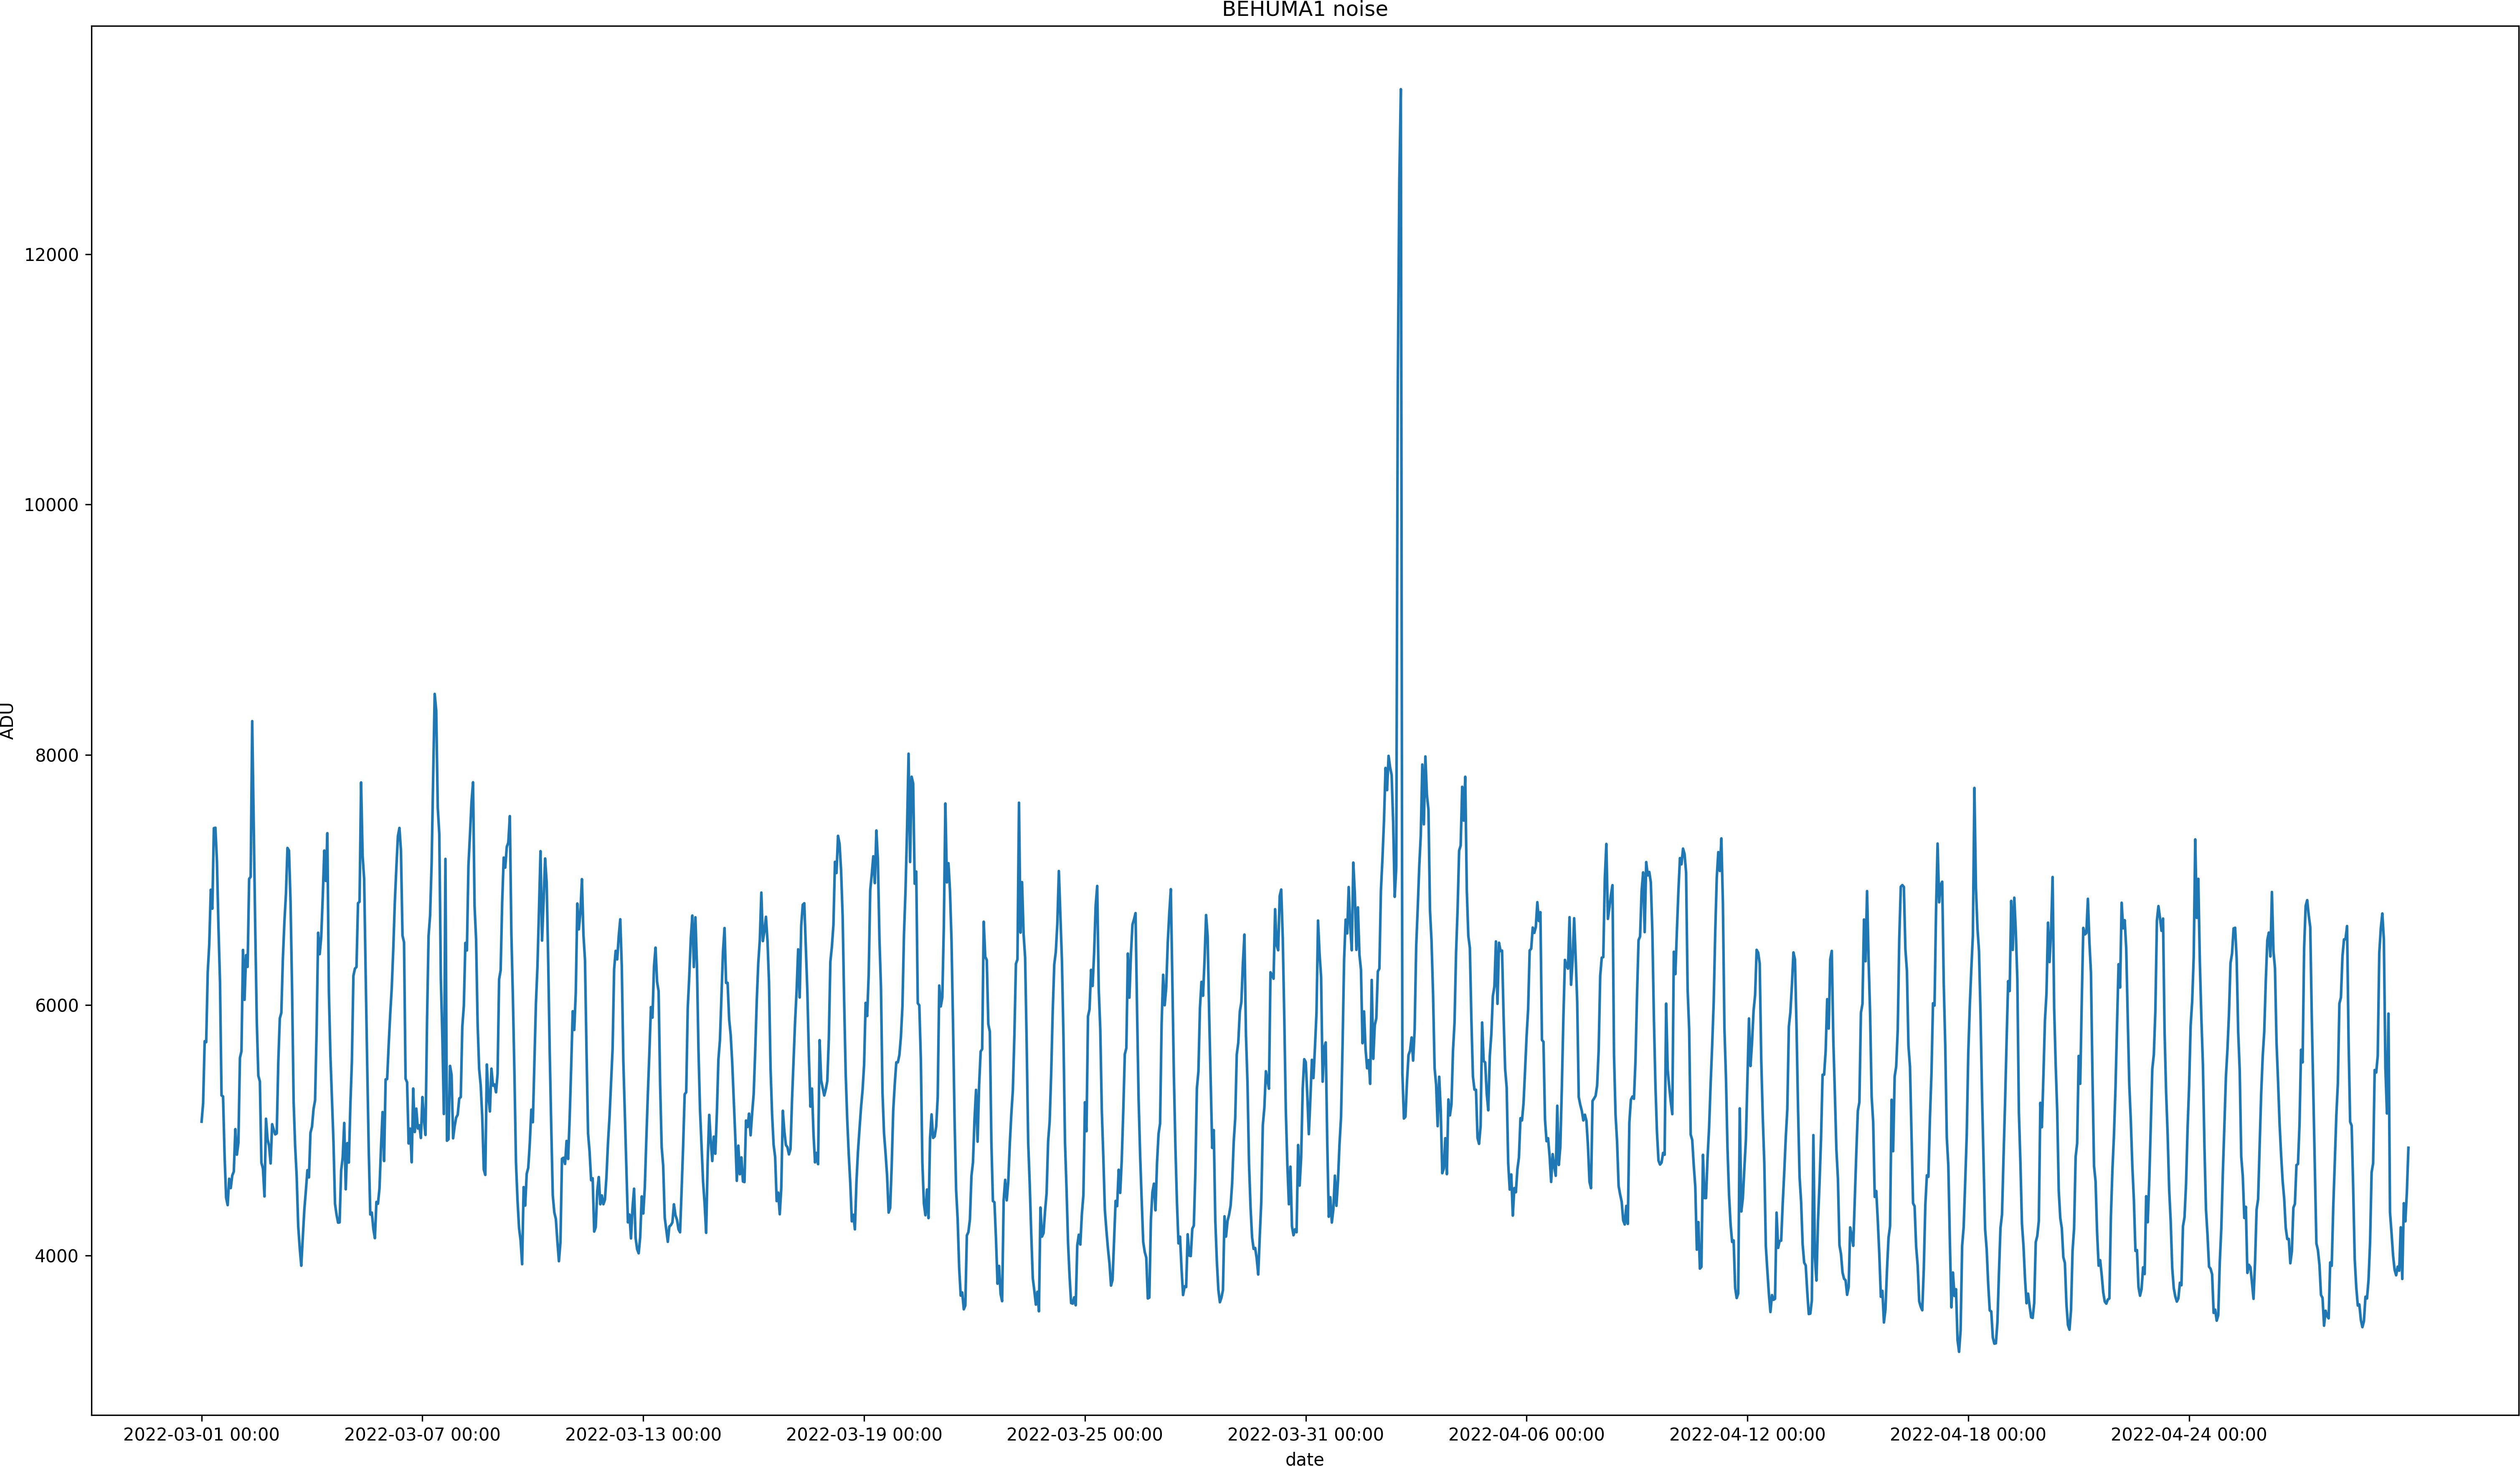
\includegraphics[scale=0.225]{page_garde.png}\\
        \vspace{0.14cm}
        \textit{2021-2022}
    \end{center}



    \vspace*{\stretch{2.0}}
\end{titlepage}

\section*{Remerciements}
\begin{remerciements}
    Je tiens tout d'abord à remercier toutes les personnes qui m'ont aidé à réaliser ce projet de fin d'études.\\
    \par
    En commençant par mon professeur rapporteur, à qui j'ai pu poser mes questions en cas de besoin et qui s'est assuré que tout se passe bien tout au long du projet.\\
    \par
    Ensuite, je voudrais remercier Mr Hervé Lamy d'avoir proposé ce sujet, mais également d'avoir expliqué, de façon claire et précise, toutes les notions qui nécessitaient des explications.\\
    \par
    Je tiens également à remercier Mrs Antoine Calegaro et Michel Anciaux, qui m'ont guidé quand c'était nécessaire et qui m'ont conseillé durant le projet de fin d'études.\\
    \par
    Enfin, je voudrais exprimer ma reconnaissance envers toutes les personnes qui m'ont conseillé sur, et ont relu ce rapport de projet de fin d'études.
\end{remerciements}

\newpage

\tableofcontents

\newpage

\section{Introduction}

Chaque jour, des milliers d'objets passent tout près de l'atmosphère terrestre.
Parmi ces objets, on retrouve les météoroïdes : des corps pierreux ou métalliques d'une largeur pouvant varier de quelques millimètres à un mètre.
Un météoroïde, une fois rentré dans l'atmosphère, devient un météore et peut créer un phénomène lumineux connu sous le nom d' "Étoile filante".
Contrairement à ce que l'on peut penser, un météoroïde qui entre dans l'atmosphère terrestre est un événement qui se produit des milliers de fois par jour.
\\
\\
L'étude de ces météores permet de retrouver différentes informations telles que la masse ou encore la trajectoire de ceux-ci.
Ce travail de fin d'étude a pour objectif de faciliter cette étude.
Cet objectif sera accompli en permettant une visualisation facile de la qualité des données étudiées et en automatisant une partie de la détection des météores.
Mais, afin de pouvoir les étudier, il est nécessaire de les détecter avant.
Actuellement, différentes techniques existent pour détecter des météores dans l'atmosphère.
\\
\\
L'une d'entre elles est la détection à l'aide de caméras.
Ceci a l'avantage de directement voir la trajectoire du météore et facilite donc l'étude.
Cependant, elle a un grand défaut : lorsque le ciel est nuageux ou qu'il fait jour la technique est moins efficace.
De plus, lorsqu'un petit météoroïde entre dans l'atmosphère, elle ne produit pas assez de lumière pour pouvoir être détecté par une caméra.
C'est alors qu'une autre technique, celle par détection à l'aide d'ondes radio devient intéressante.
\\
\\
Ce travail de fin d'études s'appliquera sur cette deuxième technique.
Il accomplira son objectif en automatisant et facilitant deux étapes du traitement des données produites par la détection de météores à l'aide d'ondes radios.
Notamment la détection des météores et la détection de données erronées.\\
\\
À titre plus personnel, ce travail me permettra de prouver mes capacités à réaliser un projet d'une grande ampleur en autonomie.
De plus, il aidera également à mieux m'orienter dans les années à suivre.

\newpage

\section{Détection des météores par ondes radios}

\begin{figure}[t]
    \begin{center}
        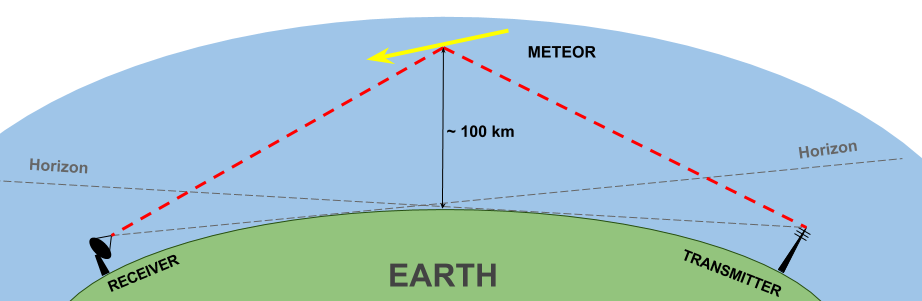
\includegraphics[scale=0.37]{ForwardScatter_principle.png}
        \caption{Détection d'un météore à l'aide d'ondes radios.}
        \label{fig:forward_scatt}
    \end{center}
\end{figure}

Quand un météoroïde entre dans la partie haute de l'atmosphère (approximativement à 80 - 120 km de la surface terrestre), il laisse derrière lui une trainée ionisée.
Cette trainée a la propriété de réfléchir les ondes radio.
On peut donc détecter un météore à l'aide de sa trainée ionisée.
\\
\\
Afin d'exploiter cette réflexion, il nous faut un émetteur dont le signal radio est réfléchi à l'aide de la trainée d'un météore et est ensuite enregistré par un récepteur.
Cette procédure est illustrée à la figure \ref{fig:forward_scatt}, où la flèche jaune représente la trainée ionisée produite par le météore.
Le signal reçu par l'émetteur est alors appelé un écho de météore.
Un écho de météore peut durer entre 1 et 10 secondes, selon la durée d'existence de la trainée ionisée.
\\
\\
Une caractéristique importante de cette technique de détection est la réflexion spéculaire.
Ceci veut dire que la trainée ionisée du météore agit comme un miroir sur lequel la réflexion se produit uniquement à un point précis, appelé le point de réflexion spéculaire.
Le point de réflexion spéculaire dépend de la position de l'émetteur, la position du récepteur et la trajectoire du météore.
La conséquence est que les données reçues par un récepteur particulier sont relatives qu'à une partie précise de la trainée.

\newpage

De plus, deux récepteurs, situés à des endroits différents, enregistreront un écho de météore à des instants différents puisque leurs points de réflexion spéculaire sont situés à des endroits différents sur la trajectoire.
Ceci est illustré à la figure \ref{fig:specular_reflex} où le point de réflexion P0 entre le transmetteur Tx et le récepteur Rx0 se situe à un endroit différent que le point de réflexion P1 entre le transmetteur et le récepteur Rx1.

\begin{figure}[t]
    \begin{center}
        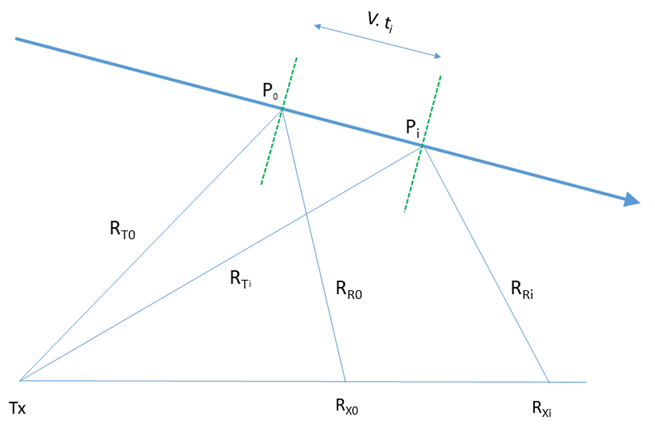
\includegraphics[scale=1]{scema_reflexion_speculaire.png}
        \caption{Le point de réflexion spéculaire est différent pour chaque station réceptrice.}
        \label{fig:specular_reflex}
    \end{center}
\end{figure}

% Pour exploiter le phénomène de la réflexion spéculaire et réussir à détecter les météores à l'aide d'ondes radios, le réseau BRAMS fonctionne de la façon suivante :
% \begin{enumerate}
%     \item Un émetteur, situé à Dourbes, transmet de façon continue un signal à une fréquence de 49.97 MHz.
%           Ce signal est émis en direction du ciel et peut être réfléchi sur des trainées ionisées dans le sillage des météores.
%     \item Lorsque le signal est réfléchi, il peut être détecté par une ou plusieurs stations réceptrices faisant partie du réseau BRAMS.
%           Un signal calibreur est alors additionné au signal venant du ciel.
%           Ce signal est injecté à 49.9705 MHz, c'est-à-dire 500 Hz plus haut que le signal direct.
%           Il dispose d'une amplitude fixe et sert de référence d'amplitude pour le reste du signal.
%           La station réceptrice décale ensuite le signal direct de 49.97 MHz vers une fréquence de 1 kHz.
%     \item Ensuite, la station réceptrice enregistre l'ensemble du signal dans un fichier audio de type WAV.
%           Le signal est échantillonné à une fréquence de 5512,5 Hz pour les stations ICOM et 6048 Hz pour les stations RSP2.
%           Si tout se passe bien, un fichier est généré toutes les cinq minutes et chaque fichier devrait commencer et terminer à un temps prédéfini (par exemple : 16 h 00 à 16 h 05, 16 h 05 à 16 h 10, etc.).
%     \item Tous les fichiers générés par les stations réceptrices sont envoyés à intervalle régulier aux serveurs utilisés pour le projet BRAMS par internet.
%     \item Une fois sur le serveur, les fichiers WAV sont archivés, manipulés et étudiés par les scientifiques du projet BRAMS afin d'en extraire les informations utiles.
% \end{enumerate}

\newpage

\begin{figure}[t]
    \begin{center}
        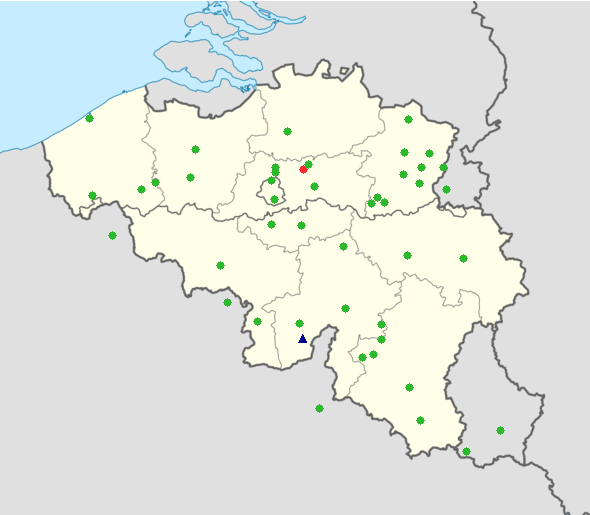
\includegraphics[scale=1]{station_map.png}
        \caption{Carte montrant l'emplacement de l'émetteur et récepteurs.}
        \label{fig:station_map}
    \end{center}
\end{figure}

\section{Le projet BRAMS}

Lancé en 2010 par Monsieur Hervé Lamy à l'Institut Royal d'Aéronomie Spatiale de Belgique, le projet BRAMS (Belgian RAdio Meteor Stations) a pour but de détecter et d'étudier les météores en utilisant la détection des météores par ondes radios.
Il dispose pour ceci d'un réseau d'un émetteur et de quarante-deux récepteurs situés dans la Belgique et dans les pays avoisinants.
Les emplacements de ces stations peuvent être visualisé sur la figure \ref{fig:station_map}, où le triangle bleu représente l'émetteur et les boules vertes sont des réceptrices.
Dans cette section, ce réseau et son fonctionnement seront expliqués.

\subsection{L'Émetteur}

Le réseau BRAMS dispose d'un émetteur unique situé à Dourbes, dans le sud de la Belgique.
Cet émetteur transmet de façon continue un signal à la fréquence 49.970 MHz et d'une puissance d'approximativement 120 W.
Ce signal sera réfléchi sur d'éventuelles trainées de météores et pourra être détecté par des récepteurs.

\subsection{Les Stations de Réception}

Les stations réceptrices permettent donc de récupérer le signal de l'émetteur, réfléchi par les échos de météores.
Durant la période d'existence du projet BRAMS, plusieurs stations réceptrices ont été développées.
Actuellement, le réseau BRAMS est composé de deux types de stations différentes.
Ces deux stations réceptrices et leurs différences seront expliquées ci-dessous.

\begin{figure}[h]
    \begin{center}
        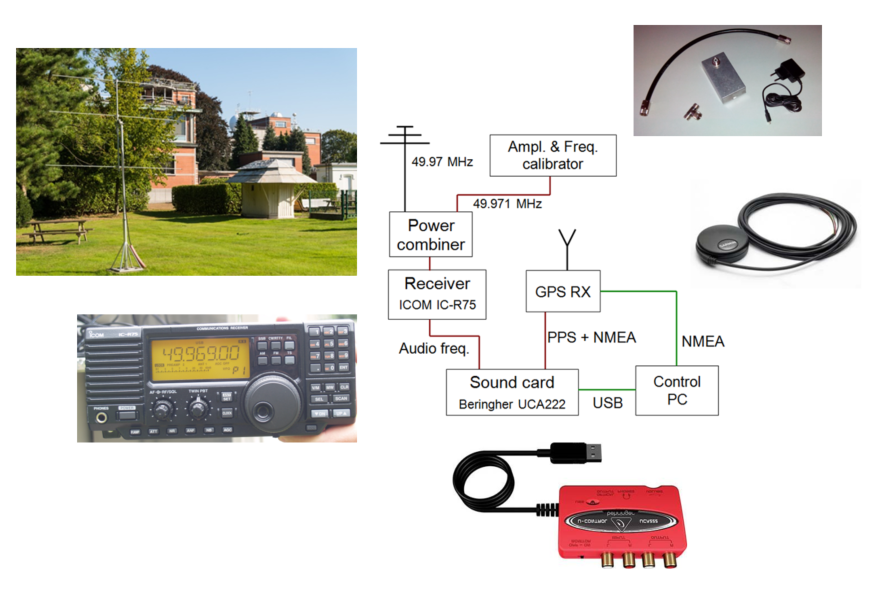
\includegraphics[scale=0.6]{Material_BRAMS_1.0.png}
        \caption{Station v1 du réseau BRAMS}
        \label{fig:station_icom}
    \end{center}
\end{figure}

\subsubsection{Les Stations V1}

Les premières stations utilisent des récepteurs analogiques ICOM-R75.
Dans ce récepteur sont injectés le signal venant de l'antenne à 49,97 MHz et le signal calibreur généré par un appareil présent dans la station réceptrice.
Le signal calibreur est constant et dispose d'une fréquence de 49,975 MHz (500 Hz au-dessus du signal de l'antenne).
Elle est additionnée au signal de l'antenne à l'aide d'un simple T.
Ce signal calibreur a un but bien précis : permettre la conversion des valeurs reçues par le récepteur en unités Watts.
Comme on connait sa puissance, elle sert de référence et nous permet de calculer la puissance des autres signaux captés par l'antenne.

\newpage

Le récepteur décale le signal reçu par l'antenne et le calibreur à 1 kHz à l'aide de l'oscillateur local réglé à 49,969 MHz.
Le signal passe ensuite par une carte son externe, où il est échantillonnée à un taux de 22050 Hz.
Cette carte son est également connectée à une horloge GPS\footnote{Global Positioning System} Garmin.
L'horloge ajoute un signal de 1 PPS \footnote{Pulse Per Second} suivi de données NMEA \footnote{National Marine Electronics Association} au signal reçu par l'antenne.
Les données NMEA contiennent, entre autres, les informations à propos de la seconde associée au dernier PPS (horodatage).
Ceci permet d'avoir un temps très précis pour chaque échantillon du signal.
\\
\\
La carte son est ensuite connectée à un ordinateur faisant tourner le logiciel 'Spectrum Lab'.
Ce logiciel pilote la station et gère la procédure permettant de détecter des échos de météores.
Afin de synchroniser l'horloge de l'ordinateur, celui-ci est également connecté à l'horloge GPS.
Les données récupérées sont enregistrées toutes les cinq minutes dans des fichiers de format WAV\footnote{Waveform Audio File}.
La figure \ref{fig:station_icom} montre un schéma de la station v1.\\
\\
Ces stations ont parfaitement fonctionné pendant longtemps.
Cependant, un problème avec le récepteur ICOM s'est manifesté de façon récurrente à partir de 2017.
Remplacer ces récepteurs s'est avéré compliqué comme le récepteur ICOM n'était plus produit.
D'autres récepteurs analogiques pouvaient servir comme remplaçant, mais ceux-ci étaient bien plus chers.
%? confrontée ?
De plus, la station v1 était confrontée à plusieurs autres problèmes comme une faible portabilité ou encore une installation complexe.
Ceci a poussé les membres du projet BRAMS au développement d'une nouvelle solution permettant de remplacer les stations v1.

\begin{figure}[h]
    \begin{center}
        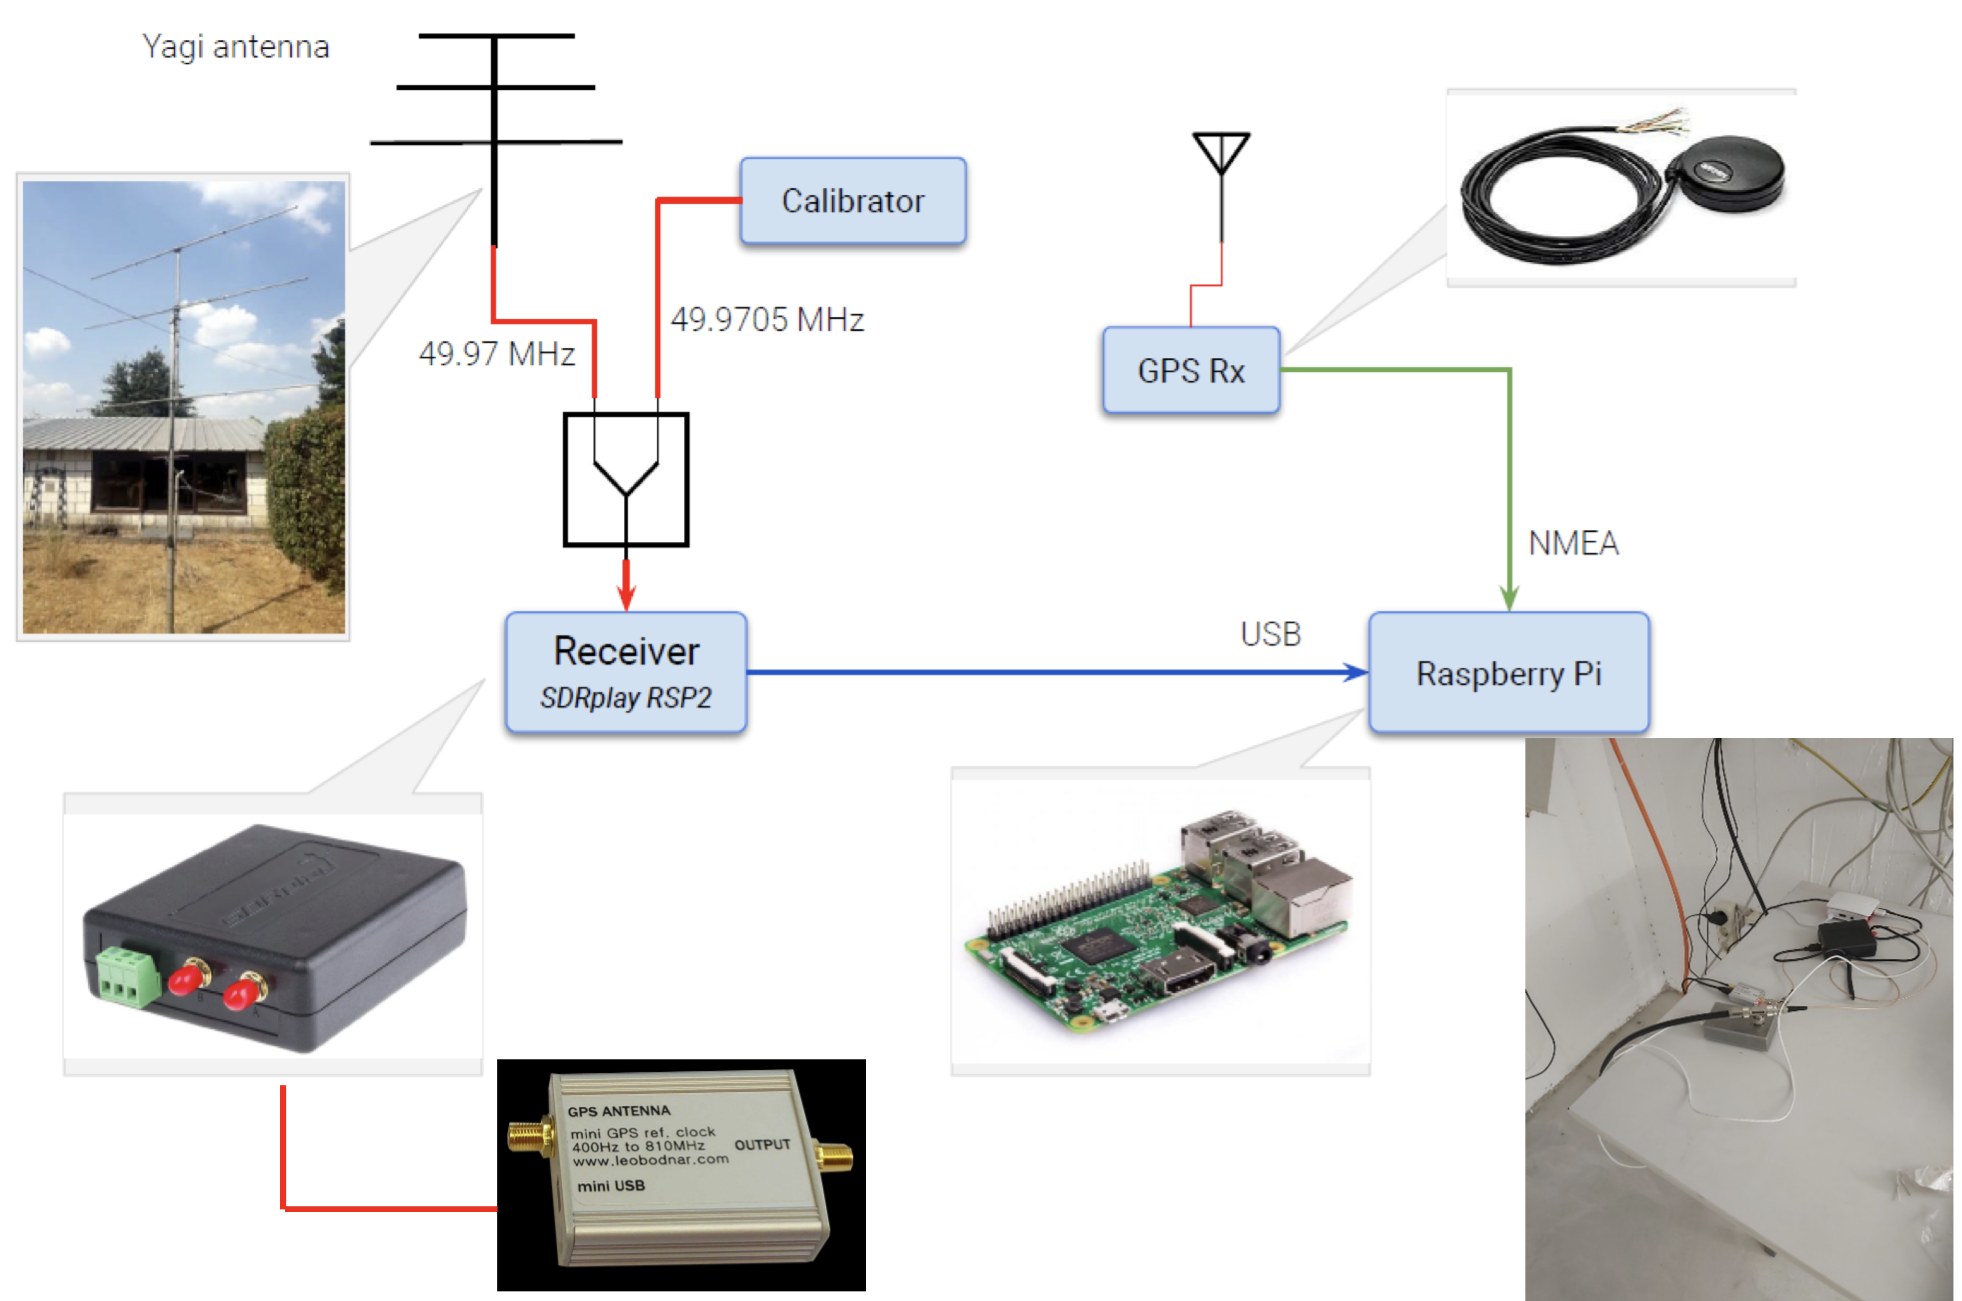
\includegraphics[scale=0.3]{schema_rsp2.png}
        \caption{Station v2 du réseau BRAMS.}
        \label{fig:station_rsp2}
    \end{center}
\end{figure}

\subsubsection{Les Stations V2}

En 2017 un étudiant venant de l'Ephec, nommé Antoine Calegaro, a créé un prototype d'une nouvelle station.
À partir de ce prototype Michel Anciaux, membre du projet BRAMS, a développé la station v2, destiné à remplacer les stations v1\\
\\
La station v2 est piloté par un Raspberry PI dont l'horloge est synchronisé avec le signal PPS du même GPS Garmin utilisé sur la station v1.
Son récepteur est un RSP2 qui à l'avantage d'avoir une portée dynamique plus grande et une sensibilité supérieure par rapport au récepteur ICOM.
Il est également moins cher que son prédécesseur.
Cependant, il ne permet pas l'échantillonnage du signal de l'antenne ensemble avec le signal GPS de 1 PPS.
La fréquence du récepteur est stabilisé à l'aide d'une fréquence de référence externe à 24 MHz donné par un GPSDO\footnote{GPS Disciplined Oscillator}.\\
\\
L'utilisation de deux horloges GPS (un pour le timing sur le Raspberry et un pour la fréquence sur le récepteur) permet d'avoir la fréquence de l'émetteur exactement à 1 kHz et le signal calibreur exactement 500 Hz au-dessus.
Ceci était un problème sur les anciens récepteurs qui ne permettaient pas de stabiliser la fréquence à l'aide d'une source extérieure, causant des dérives de fréquence selon la température de celui-ci.
La figure \ref{fig:station_rsp2} montre un schéma des composants de la nouvelle station réceptrice.
En 2020, la station fut placée dans une boite métallique et la fréquence de référence du GPSDO fut également utilisé pour stabiliser l'oscillateur local du calibreur.\\
\\
Cette station est donc beaucoup plus simple à installer puisqu'elle ne nécessite plus d'ordinateur externe pour son fonctionnement.
En plus d'être plus compact et facile à installer que la station v1, la station v2 améliore la qualité des données et est moins cher.


% Il existe 2 types de station de réception :
% % ! the part below should be divided in 2 subtitles and should also be developped more
% \begin{itemize}
%     \item Il y a d'abord les stations avec des récepteurs Icom IC-R75, que j'apellerai les récepteurs ICOM dans ce document.
%           Ce sont les premières stations réceptrices mises en service pour le réseau BRAMS.
%           Actuellement, ces stations ne sont plus utilisées suite à l'arrêt de la commercialisation du récepteur Icom IC-R75.
%           De plus, une variation de température pouvait causer une légère déstabilisation en fréquence.
%     \item C'est alors que les stations utilisant le récepteur RSP 2 ont été développés.
%           Ces stations n'éliminaient pas seulement en grande partie les problèmes des anciennes stations, mais sont également plus compacts et plus faciles à installer.
%           Une image des stations RSP 2 peut être trouvé à la figure 1.
% \end{itemize}

% \subsubsection{Le Format WAV}

% Le format de fichier WAV (Waveform Audio File) est un format destiné au stockage de signal audio développé par Microsoft et IBM.
% Il est construit conformément au RIFF (Ressource Interchange File Format) ce qui veut dire que le fichier est organisé en blocs de données, aussi nommés des "chunks" ou "data chunks".\\
% \\
% Chaque bloc de données dispose d'un ID codé sur 4 octets, qui représente souvent un mot de 4 lettres.
% Suit ensuite le champ "subChunkSize" indiquant la taille des données à venir dans le bloc de données, codé également sur 4 octets.
% Cette valeur exclut donc les champs "ID" et "subChunkSize" du bloc courant.
% Après ces 2 champs, on est libre de rajouter le nombre de champs que l'on souhaite, avec la taille en octets que l'on souhaite.\\
% \\
% Pour un fichier WAV, on retrouve typiquement 3 blocs de données.
% On retrouve premièrement le bloc "RIFF", dont le champ "ID" contient les quatre lettres "RIFF".
% Ce bloc est particulier puisque, au lieu d'avoir un champ "subChunkSize", il a un champ "ChunkSize".
% La différence est que, contrairement au champ "subChunkSize", le champ "ChunkSize" contient la taille de l'entièreté du fichier, exclu le champ "ID" et le champ "ChunkSize" même du bloc "RIFF".
% Vient ensuite le champ "format", ce champ indique le type de fichier actuel.
% Dans le cas du fichier WAV, ce dernier contient les quatre lettres "WAVE".\\
% \\
% Le deuxième bloc, nommé le bloc FMT\footnote{FMT pour format}, contenu dans un fichier WAV ordinaire contient toutes les données techniques des données.
% On y trouve notamment la fréquence d'échantillonnage, le nombre de pistes audio ou encore le nombre d'octets par secondes.\\
% \\
% Vient enfin le bloc principal du fichier : le bloc de données.
% C'est dans ce bloc que se trouvent les données audio brutes.
% La taille de ce bloc varie bien-entendu selon les caractéristiques techniques des données audio (longueur, fréquence d'échantillonnage, nombre de pistes, etc.).\\
% \\
% Une chose à noter à propos des fichiers WAV est que leur structure offre une grande flexibilité.
% En effet, elle permet non-seulement de lire et interpréter les fichiers facilement, mais également de rajouter des blocs de données personnalisés sans corrompre les autres données.\\
% \\
% La figure 2 montre la structure d'un fichier WAV ordinaire.

% \begin{figure}[t]
%     \begin{center}
%         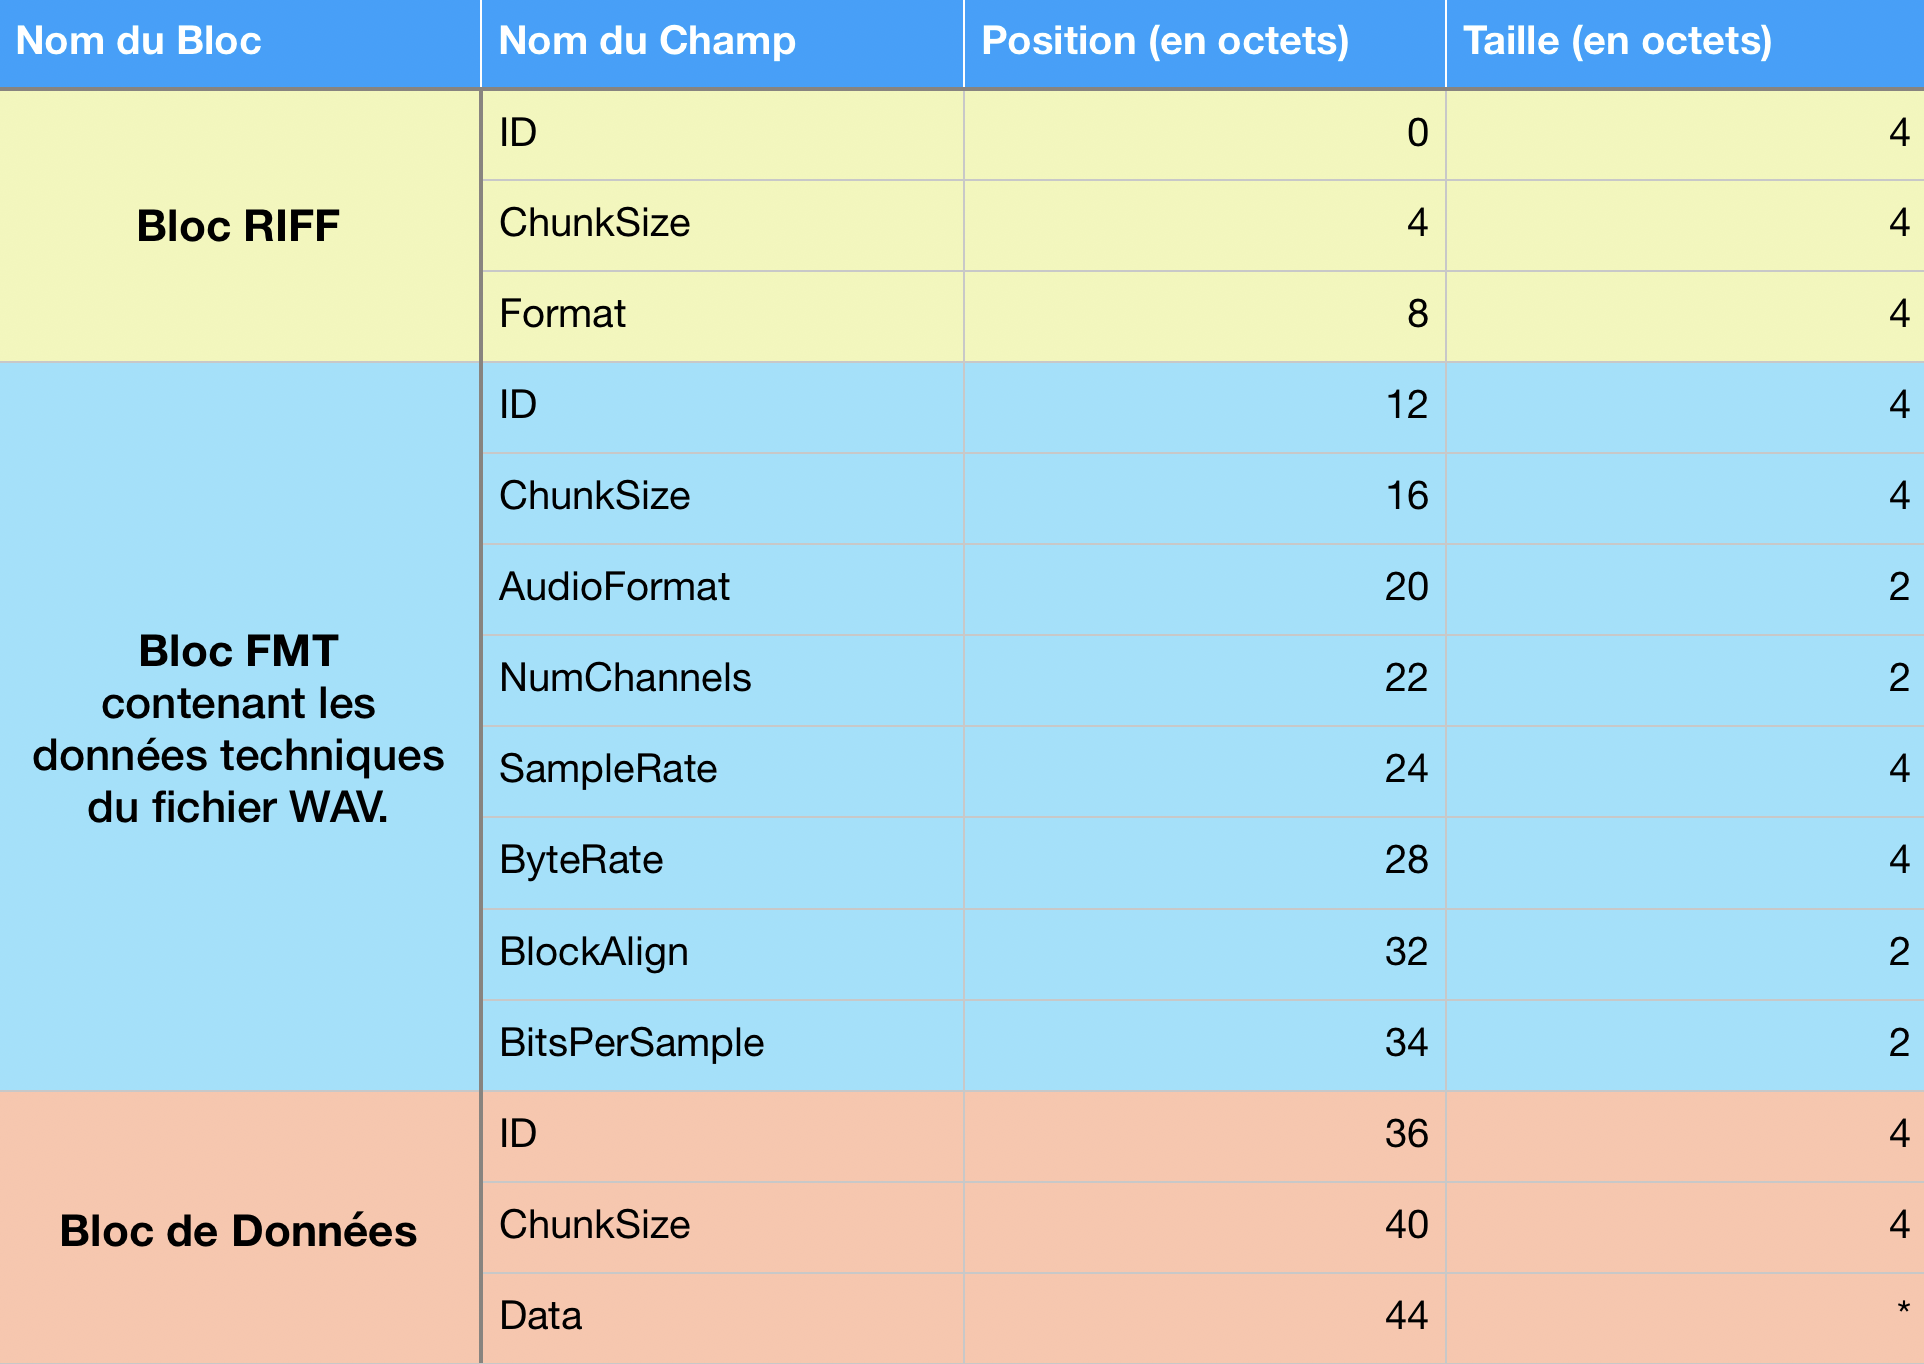
\includegraphics[scale=0.3]{wav_structure.png}
%         \caption{Structure d'un fichier WAV ordinaire}
%     \end{center}
% \end{figure}

% \newpage

\subsection{Les Données BRAMS}

Un fichier WAV venant d'une station réceptrice contient donc le signal capté par l'antenne ensemble avec un signal calibreur.
Il est composé d'une seule piste audio, échantillonnée à une fréquence de 5512.5 Hz pour les stations v1 ou 6048 Hz pour les stations v2.
Cette fréquence permet d'enregistrer des données dans une bande de fréquences allant jusqu'à respectivement 2756.25 Hz ou 3024 Hz (ou la moitié de la fréquence d'échantillonnage), selon le théorème de Nyquist.
Sachant que les échos de météores apparaissent typiquement dans une bande de fréquence de 100 Hz autour du signal de l'émetteur qui est décalé à 1000 Hz, cette bande de fréquence couvre l'ensemble des signaux utiles à l'étude des météores.\\
\\
À chaque fichier WAV est rajouté un bloc de données (data chunk) conçu pour faciliter l'étude des signaux capturés par la station.
Dans ce bloc, on retrouve quelques informations relatives à la station de réception, la station émettrice, le signal GPS ou encore, la fréquence d'échantillonnage.

\begin{figure}[h]
    \begin{center}
        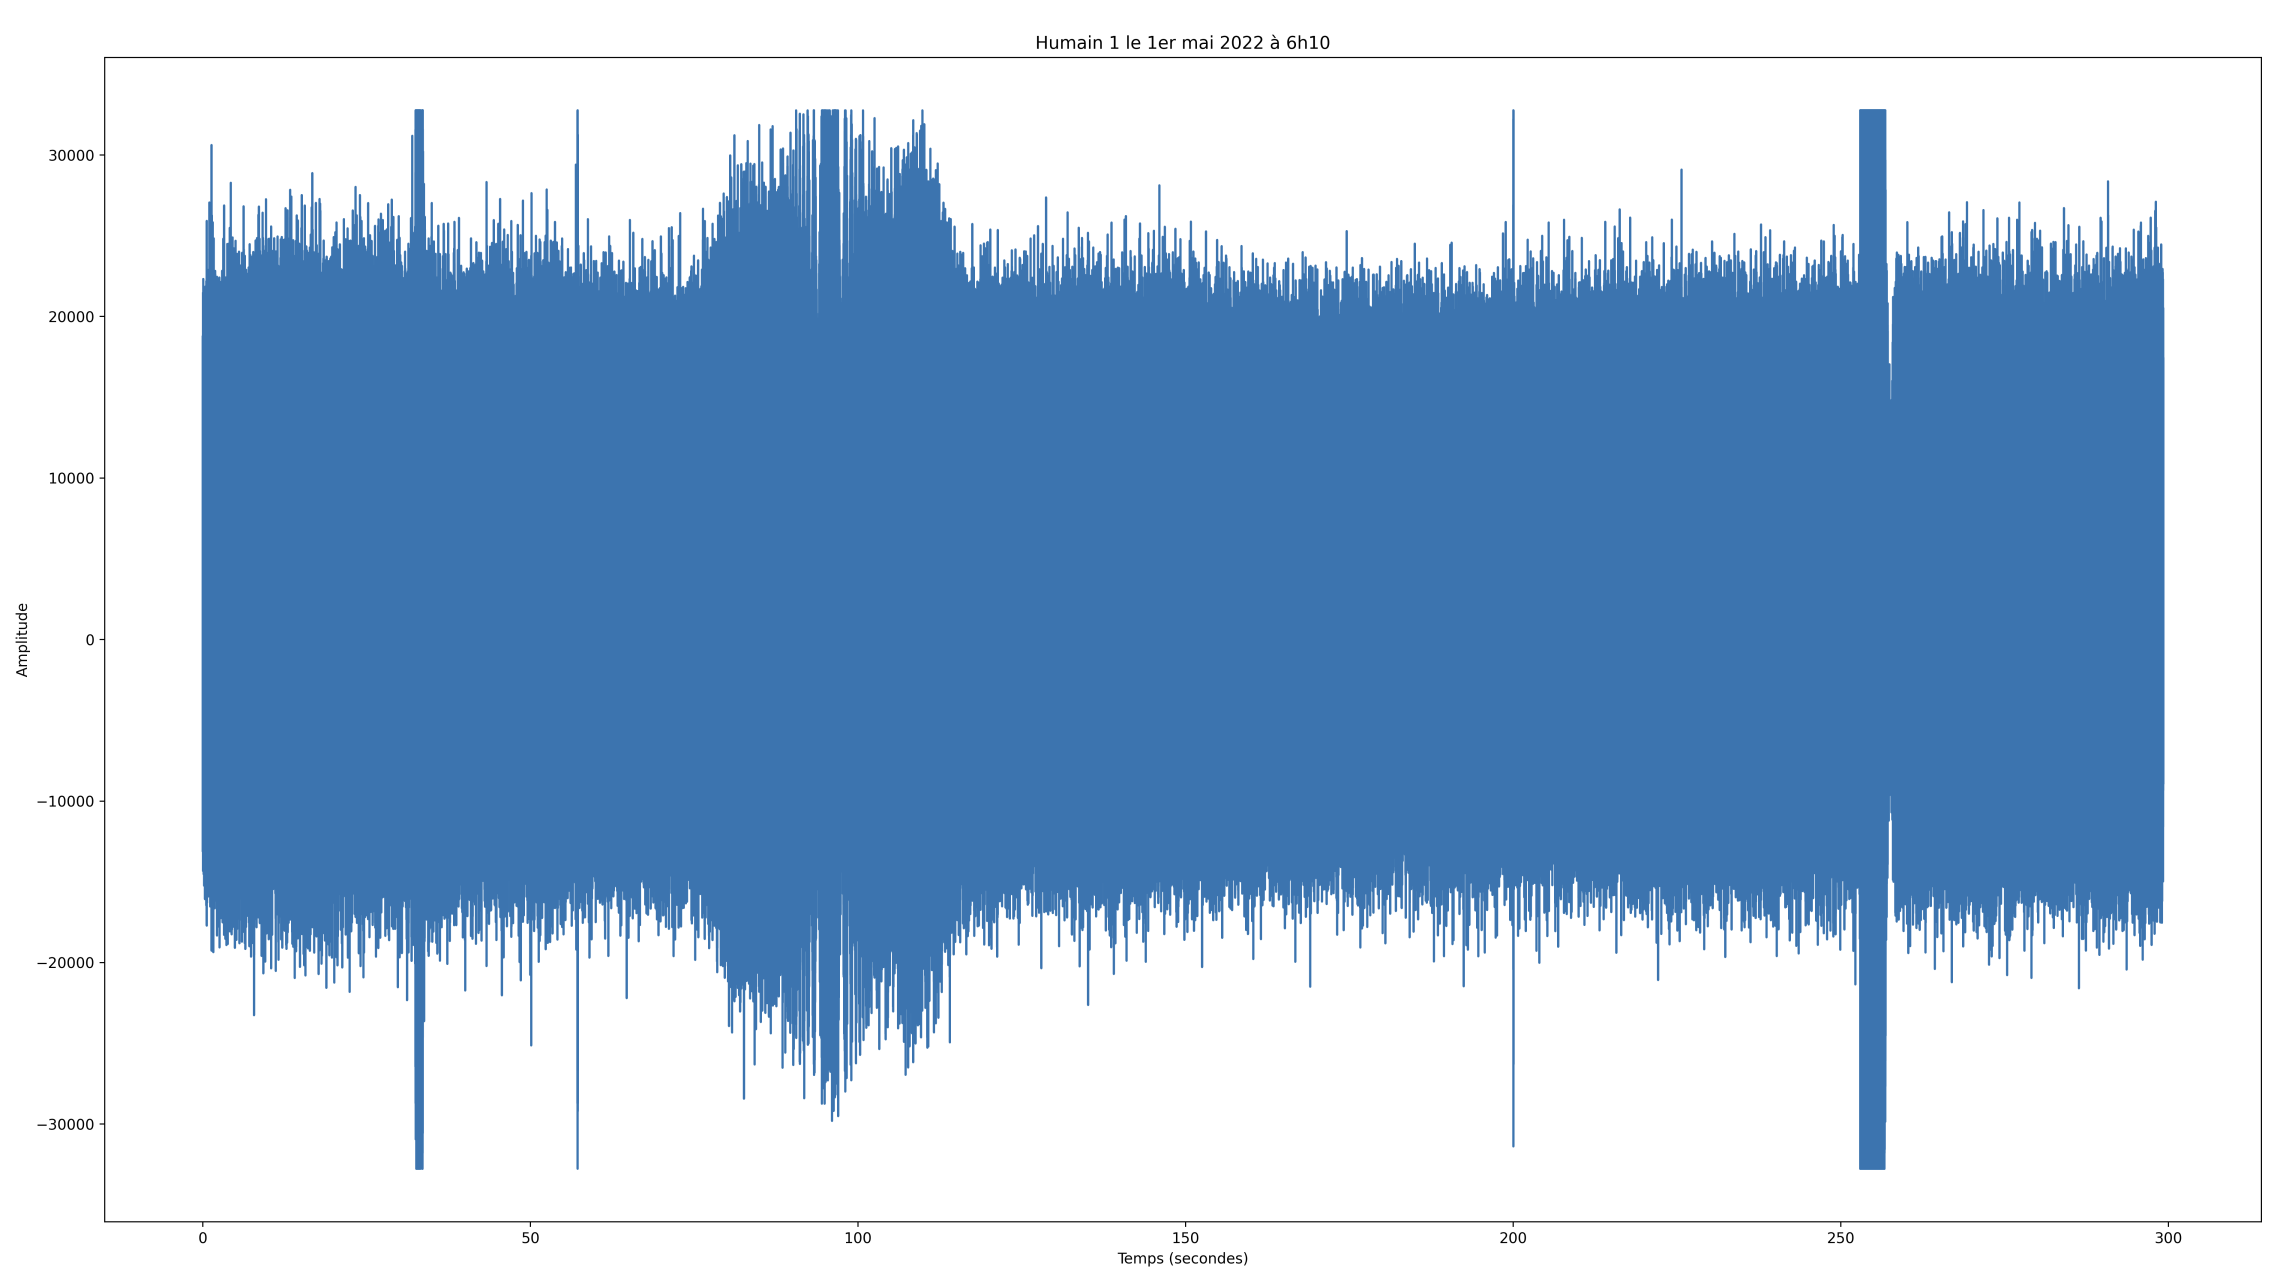
\includegraphics[scale=0.155]{wav_brut.png}
        \caption{Données brutes venant d'un fichier audio d'une station réceptrice.}
        \label{fig:wav_brut}
    \end{center}
\end{figure}

%? montré?
Ces fichiers audio, comme montré à la figure \ref{fig:wav_brut}, sont très difficiles à interpréter.
Ils sont composés de bruits et de parasites sur l'entièreté de leur bande de fréquence.
Par contre, lorsque l'on calcule le spectrogramme du fichier WAV, les données deviennent beaucoup plus simples à lire.
\\
\\
Un spectrogramme est une représentation différente des données contenues dans un fichier audio.
Au lieu de représenter l'intensité sur l'ordonnée et le temps sur l'abscisse, un spectrogramme représente la répartition des fréquences au cours du temps.
Il contient donc trois dimensions :
\begin{itemize}
    \item Le temps sur l'abscisse.
    \item La fréquence sur l'ordonnée.
    \item L'intensité représentée par un code couleur.\\
\end{itemize}

\begin{figure}[h]
    \begin{center}
        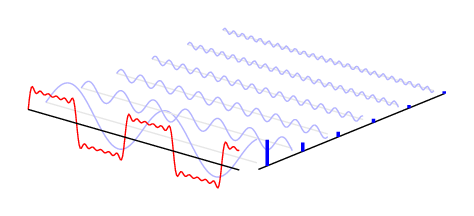
\includegraphics[scale=0.7]{spectre.png}
        \caption{Représentation visuelle de la Transformée de Fourier.}
        \label{fig:expl_fourier}
    \end{center}
\end{figure}

Pour générer un spectrogramme, il faut calculer un ensemble de Transformées de Fourier.
La Transformée de Fourier permet de représenter la répartition de puissance entre les fréquences contenues dans un signal ou une partie d'un signal temporel.
Elle produit donc ce qu'on appelle le spectre du signal.
Elle se calcule sur un nombre quelconque d'échantillons qui se suivent dans un signal temporel.
Ce spectre est souvent calculé à l'aide de la FFT\footnote{Fast Fourier transform} qui est plus rapide, mais qui exige un nombre d'échantillons $2^{n}$.\\
\\
Sur la figure \ref{fig:expl_fourier}, on peut observer en rouge un signal temporel et le spectre de ce même signal en bleu.
Les signaux en mauve clair sont les signaux à une fréquence, dont le signal rouge est composé.

\begin{figure}[h]
    \begin{center}
        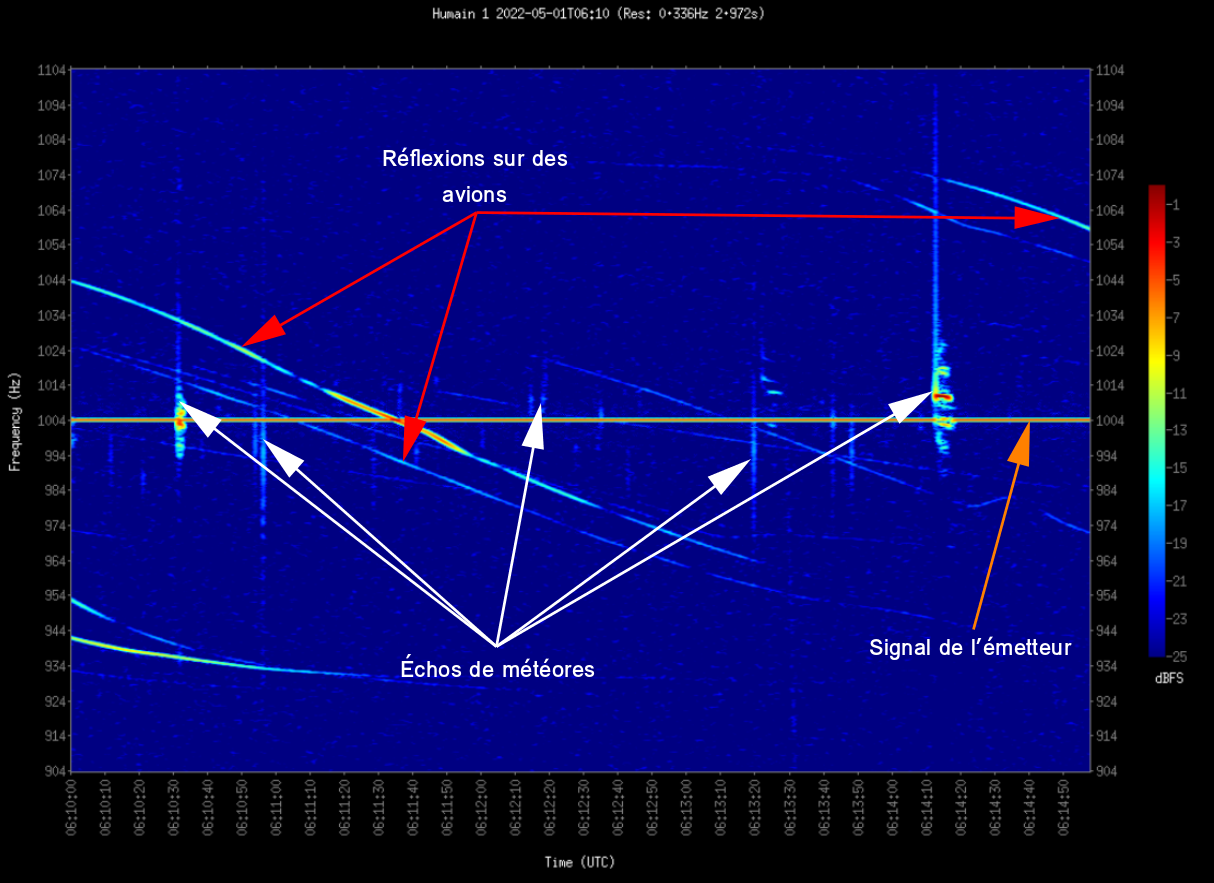
\includegraphics[scale=0.29]{spectrogramme_legend.png}
        \caption{Exemple d'un spectrogramme du projet BRAMS de 900 Hz à 1100 Hz. Les données représentées sont les mêmes qu'à la figure \ref{fig:wav_brut}}
        \label{fig:spectro_brams-a}
    \end{center}
\end{figure}

Dans le cas des spectrogrammes pour le projet BRAMS, les FFT sont calculés sur 16384 échantillons.
Si on suppose qu'un fichier WAV venant d'une station réceptrice dure en moyenne trois-cents secondes (ou cinq minutes), un spectrogramme est composé d'environ 101 spectres pour les stations v1 et 111 pour les stations v2.
Ce nombre est obtenu avec la formule ci-dessous, où Fs est la fréquence d'échantillonnage, T la durée en secondes du signal et nfft le nombre d'échantillons utilisés pour générer un spectre.
\[\frac{Fs * T}{nfft}\]
Le spectrogramme généré aura une résolution fréquentielle, donnée par la formule \(Fs / nfft\), de 0.34 Hz pour les stations v1 et 0.37 Hz pour les stations v2.
Sa résolution temporelle, donnée par la formule \(nfft / Fs\), est de 2.97 secondes pour les stations v1 et de 2.7 secondes pour les stations v2.
Un exemple de spectrogramme venant d'une station de réception est affiché aux figures \ref{fig:spectro_brams-a} et \ref{fig:spectro_brams-b}.
Sur la figure \ref{fig:spectro_brams-a}, on voit la partie du spectrogramme entre les fréquences de 900 Hz et 1100 Hz.
Dans cette partie sont contenues les échos de météores, le signal direct de l'émetteur à environ 1000 Hz et des parasites qui sont typiquement des réflexions sur les avions.
On y retrouve donc tout le signal utile.
Sur la figure \ref{fig:spectro_brams-b} on voit l'entièreté (0 Hz - 3000 Hz) du même spectrogramme affiché à la figure \ref{fig:spectro_brams-a}.
Le contenu de cette dernière se trouve alors entre les deux lignes rouges.
On retrouve, sur la figure \ref{fig:spectro_brams-b} le signal du calibreur à environ 1500 Hz.
En-dehors des lignes orange, on peut observer que le signal est filtré.
Ce filtrage est automatique et est appliquée sur tous les fichiers WAV du projet BRAMS.

\begin{figure}[h]
    \begin{center}
        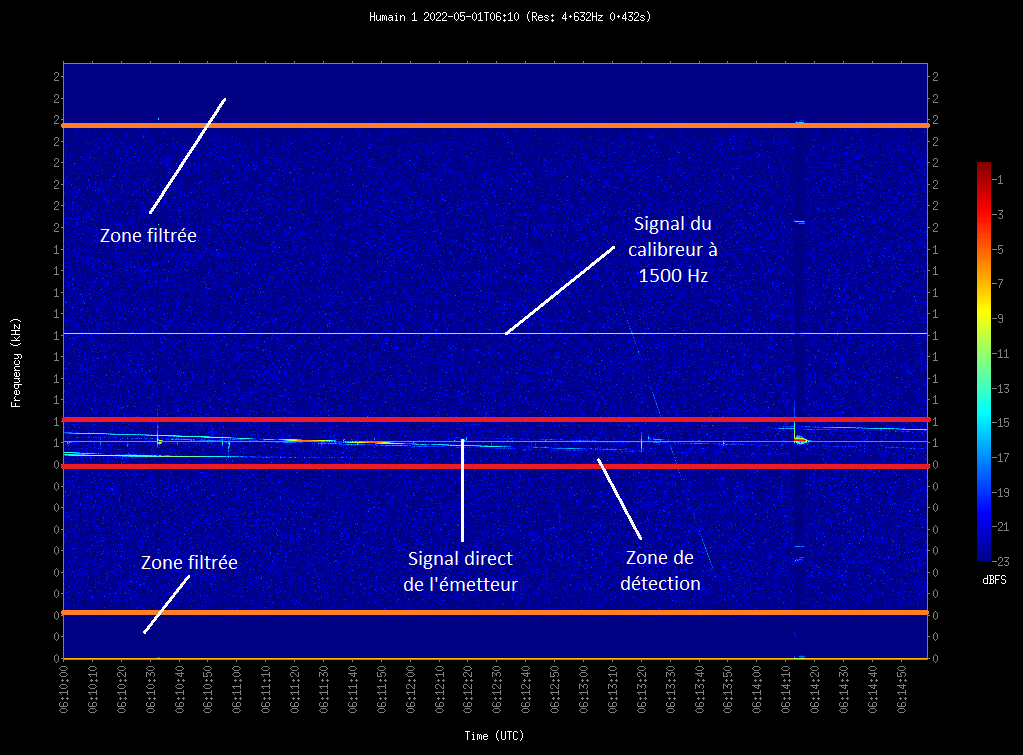
\includegraphics[scale=0.81]{RAD_BEDOUR_20220501_0610_BEHUMA_SYS001.png}
        \caption{Exemple d'un spectrogramme du projet BRAMS de 0 Hz à 3000 Hz. Les données représentées sont les mêmes qu'à la figure \ref{fig:wav_brut}}
        \label{fig:spectro_brams-b}
    \end{center}
\end{figure}

\subsection{L'Archive BRAMS}

Les stations réceptrices produisent donc, en théorie, un fichier WAV toutes les cinq minutes.
Ces fichiers ne sont bien évidemment pas stockés sur les stations mêmes, mais sont envoyés à intervalle régulier aux serveurs dédiés du projet BRAMS.
Les fichiers qui arrivent aux serveurs sont archivés une fois par jour.
Cette procédure d'archivage est activée manuellement en lançant un script bash.\\
\\
Quand les fichiers venant des stations de réception sont archivés, ils sont placés dans une structure de répertoires spécifique.
Le chemin pour accéder à un fichier WAV spécifique et son nom dépendent de la station d'où vient le fichier ainsi que la date de début d'enregistrement du fichier.
C'est grâce à ces noms de fichiers, dont vous trouverez un exemple à la figure \ref{fig:file_name_brams}, et cette structure fixe qu'on peut retrouver facilement chaque fichier au sein de l'archive.\\

\begin{figure}[t]
    \begin{center}
        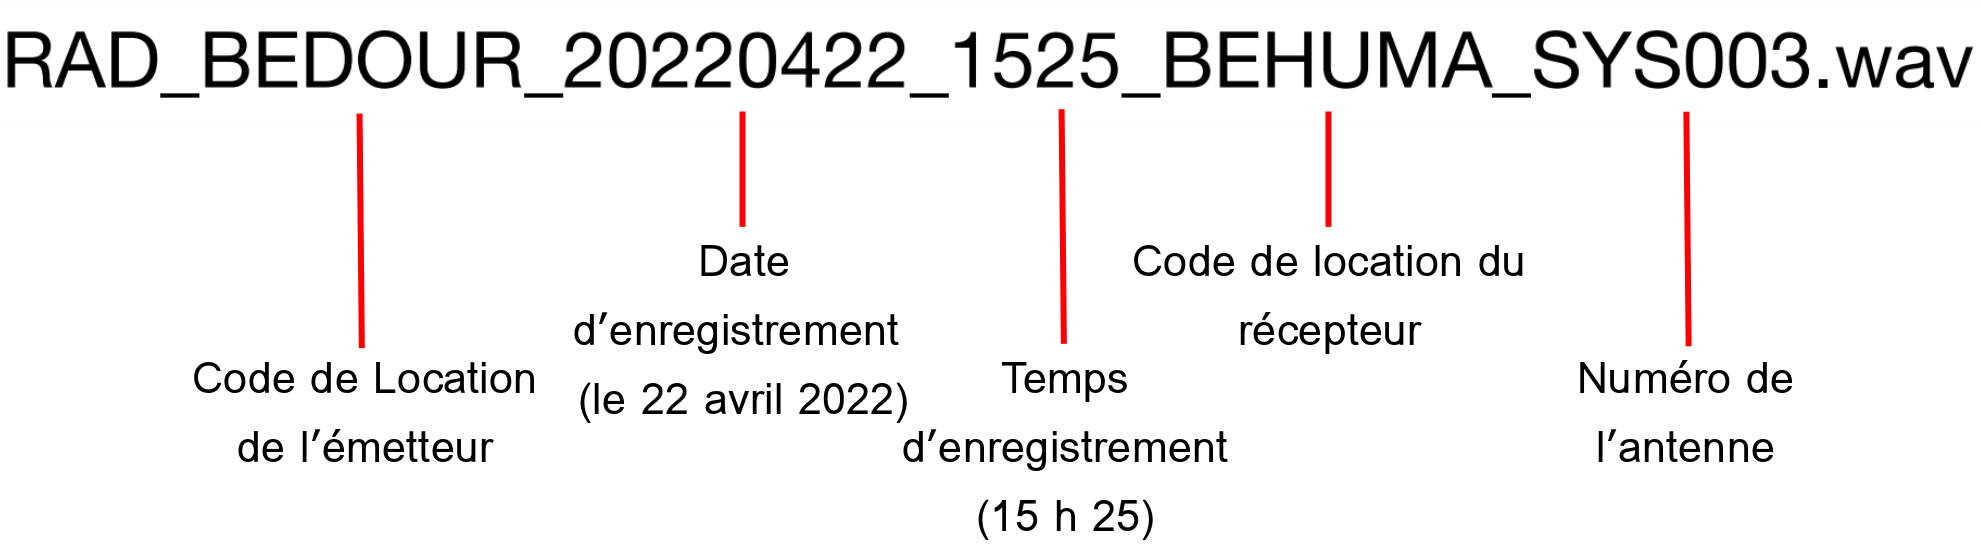
\includegraphics[scale=0.15]{file_name.png}
        \caption{Exemple de nom de fichier BRAMS.}
        \label{fig:file_name_brams}
    \end{center}
\end{figure}

\newpage

\section{Problématique liée à l'étude des données BRAMS}

Le but du projet BRAMS est donc d'étudier les fichiers WAV venant des stations réceptrices afin de retrouver, entre autres, la trajectoire des météores.
Pour identifier ces trajectoires, il est d'abord nécessaire de récupérer tous les fichiers contenant un écho de ce météore.
C'est une action qui demande beaucoup de temps puisque l'utilisateur doit pour cela ouvrir chaque fichier de toutes les stations et vérifier s'il y a bien écho venant du météore.\\
\\
De plus, actuellement il n'existe aucune façon de détecter une station produisant des données erronées.
%? aperçoit vs aperçoive?
Ceci veut dire qu'une station pourrait produire des fichiers inutilisables pendant plusieurs mois sans que personne ne s'en aperçoit.
Ces fichiers prendraient non-seulement de l'espace de stockage inutilement, mais dans le cas où une étude nécessiterait les données de cette station, elle seraient inutilisables.\\
\\
C'est pour ces deux raisons que les membres du projet BRAMS souhaitent faciliter et automatiser certaines étapes dans l'étude des données BRAMS.
Ils ont donc demandé à réaliser une ou plusieurs solutions permettant les actions suivantes :

\begin{itemize}
    \item La détection la plus précise des échos d'un météore dans les fichiers de stations réceptrices différentes.\\
          Le résultat du programme doit être un fichier de format CSV\footnote{Comma Separated Values} qui indique chaque écho dont le programme pense qu'il vient du météore recherché.
          Pour chaque écho retenu il faut bien entendu également ajouter des informations telles que la station où il a été détecté ou encore le temps de détection.
    \item Le monitoring constant des données des différentes stations à l'aide d'une interface sur le site web du projet BRAMS.
          Ce monitoring doit permettre aux scientifiques du projet de détecter facilement une anomalie dans les données.
    \item L'avertissement par mail si une anomalie est détectée dans les données BRAMS.
          Cette action implique également la détection automatique d'anomalies dans les données venant des stations réceptrices.
\end{itemize}

\newpage

\section{Méthodologie}

Afin d'arriver à un résultat final de qualité et qui est conforme aux requis des membres du projet BRAMS, il est important d'utiliser une bonne méthodologie.\\
\\
La première étape consistait à assimiler correctement de quoi le programme doit être capable.
Pour cela, plusieurs réunions ont eu lieu avant la réalisation du travail.
Durant ces réunions, j'ai pu poser mes questions et demander des explications sur les concepts à connaître pour pouvoir réaliser le travail.
Ayant reçu des documents expliquant de façon claire et précise le fonctionnement du réseau BRAMS, j'ai pu me préparer avant de m'attaquer à l'analyse et la réalisation du travail.\\
\\
Durant la période d'analyse et de réalisation du TFE, j'ai régulièrement pu demander validation quant à la direction que je prenais pour mon travail.
Je présentais fréquemment mes réalisations aux scientifiques du projet BRAMS afin d'avoir un feedback constant et de pouvoir perfectionner mon programme un maximum.\\
\\
Dans le but d'être plus efficace lors de l'écriture des fonctionnalités pour le programme, je décrivais à l'avance ce dont la fonctionnalité devait être capable.
Ensuite, je la divisais en tâches techniques afin de pouvoir m'organiser plus facilement.
Chaque tâche technique contenait et expliquait les étapes que le programme devrait exécuter pour accomplir cette même tâche.
Les étapes étaient décrites textuellement, par pseudo-code, par schéma ou encore, par le mélange de deux ou trois des moyens cités.\\
\\
Durant l'entièreté du projet de fin d'études, j'ai tenté de garder un rythme de travail régulier.
Je me suis organisé de telle façon à pouvoir travailler en moyenne deux jours par semaine.
Une grande partie de ces heures se sont déroulés lorsque je rentrais de mon stage ou pendant le week-end.\\
\\
À la fin de ce projet de fin d'études l'entièreté du code a été donné aux membres du projet BRAMS.
Comme demandé, le code est commenté et accompagné d'un mode d'emploi.

\newpage

\section{Technologies utilisées}

\subsection{Python}

Le programme réalisé est entièrement écrit en Python.
Ce choix a été pris premièrement pour les librairies performantes et open-source qu'offre Python.
En effet, des librairies comme numpy, scipy ou encore matplotib ont été très utiles pour arriver à un résultat performant et fonctionnel.
Ces librairies offrent beaucoup de flexibilité et offrent une performance élevée grâce à leur écriture en C, C++ et même en Fortran.\\
\\
Un autre avantage du Python est sa portabilité.
Puisque c'est un langage interprété, largement répandu, quasiment tous les systèmes d'exploitation le supportent.
Ceci a facilité aussi bien la phase de développement que la phase de testing du projet de fin d'études.\\
\\
Un des désavantages souvent évoqués pour Python, est que le langage est lent pour des gros traitement de données.
Cependant, dans le cas de ce travail, ceci ne fut pas un problème et les librairies utilisées étaient suffisamment rapide.
Ceci est dû, entre autres, à la nature open-source de ces librairies ainsi qu'à leur âge.
Suite à ces deux facteurs, des milliers de personnes travaillent sur ces librairies depuis plusieurs années dans le but d'optimiser le plus possible ses fonctions et méthodes.

% \subsubsection{Librairies Utilisées}

% Dans cette section sont listées toutes les librairies Python utilisés pour la réalisation du travail de fin d'études.\\
% \\
% \textbf{Argparse}\\
% Argparse est une librairie Python qui permet de facilement créer une interface ergonomique en ligne de commande.
% On spécifie les paramètres nécessaires et optionnels pour le programme qu'on crée, et lorsqu'on lance le programme, Argparse pourra retrouver les paramètres entrés par l'utilisateur.
% Il indiquera également une erreur si un paramètre obligatoire manque, ou qu'un type de paramètre n'est pas respecté.
% Argparse est une librairie installée par défaut avec Python.\\
% \\
% \textbf{CSV}\\
% La librairie CSV offre la possibilité d'écrire et de lire des fichiers CSV à l'aide d'un programme en Python.\\
% \\
% \textbf{Datetime}\\
% La librairie Datetime offre une suite de fonctions et de classes permettant la manipulation et la conversion de temps et de dates.
% Cette librairie fait partie des modules standards de Python et ne doit donc pas être installé.\\
% \\
% \textbf{Dotenv}\\
% La librairie Dotenv permet de lire les fichiers et les variables d'environnement.\\
% \\
% \textbf{GeoPy}\\
% GeoPy est une librairie Python qui facilite la recherche de coordonnées d'adresses, de villes ou encore de lieux connus.
% Elle permet également de trouver la distance entre deux lieux en donnant les coordonnées de ces endroits.\\
% \\
% \textbf{Math}\\
% Le module math offre toute une série de fonctions mathématique de base.
% Elle est installée par défaut avec Python.\\
% \\
% \textbf{Matplotlib}\\
% La librairie Python Matplotlib permet de générer des graphiques et de les enregistrer en tant qu'image.\\
% \\
% \textbf{Mysql.connector}\\
% Cette librairie permet d'établir une connexion à une base de données MySQL ou MariaDB.
% Avec cette connexion, un programme Python peut faire des requêtes à cette base de données.\\
% \\
% \textbf{NumPy}\\
% NumPy est une librairie Python utilisée lorsqu'on travaille avec des listes très larges.
% Il contient de nombreuses fonctions pour l'algèbre linéaire, les Transformées de Fourier et les matrices.
% Par rapport aux listes classiques de Python, les listes NumPy (aussi appelés des ndarray) sont beaucoup plus rapides.\\
% \\
% Ceci est dû à trois raisons principales.
% La première est que les listes NumPy sont stockés à un endroit continu dans la mémoire RAM\footnote{Random Access Memory}, ce qui permet un accès et une manipulation plus efficace des données.
% Ensuite, comme NumPy est une librairie open-source, il est continuellement adapté à des nouvelles architectures de processeurs.
% Finalement, une grande partie de la librairie NumPy est écrit dans des langages de bas niveau tels que le C, le C++ ou encore le Fortran.
% Ceci résulte à un code beaucoup plus proche du langage machine et qui est donc plus optimisé.\\
% \\
% \textbf{Os}\\
% La librairie os de Python contient une suite de fonctions permettant d'interagir avec le système d'exploitation.
% Cette librairie vient par défaut avec une installation de Python, ce qui évite de devoir l'installer lorsque nécessaire.\\
% \\
% \textbf{SciPy}\\
% Scipy est une librairie qui est basé sur la librairie NumPy.
% Elle partage donc de nombreuses fonctions et méthodes avec cette dernière et fonctionne également avec des ndarray.
% Cependant, cette librairie ajoute des fonctions pour la science des données.
% De plus, Scipy optimise des fonctions déjà présentes dans la librairie NumPy.
% Ceci permet de construire un programme qui demande moins de ressources machine et qui est donc plus rapide.\\
% \\
% \textbf{Simplejson}\\
% Simplejson est une librairie Python offrant la possibilité de facilement écrire et lire des fichiers JSON\footnote{JavaScript Object Notation}.
% Elle vient par défaut avec Python sous le nom 'json'.
% Cependant, installer Simplejson séparément ajoute l'avantage d'avoir des mises à jour plus régulières et de disposer des dernières fonctionnalités plus rapidement.\\
% \\
% \textbf{Tarfile}\\
% Le module Python Tarfile permet de lire et écrire des fichiers du format TAR.
% Cette librairie est incluse par défaut avec Python et ne doit donc pas être installé séparément.\\
% \\
% \textbf{Tqdm}\\
% Tqdm est une librairie Python permettant d'afficher des barres de chargements en ligne de commande.
% Elle permet également de donner une estimation de temps de chargement restant.\\

\subsection{MariaDB}

Afin de sauvegarder les données produites par le programme, une base de données est requise.
Les données sont enregistrées dans la base de données existant du projet BRAMS.
Le type de base de données du projet BRAMS est MariaDB.
% Les données produites seront toutes liées à un fichier, le choix d'une base de données relationnelle est donc appropriée.\\
% \\
% MariaDB est une dérivée de MySQL.
% Elle a l'avantage d'être gratuite et open-source.
% Grâce à une large communauté contribuant au développement continu de MariaDB, elle est souvent plus performante que MySQL.
% De plus, étant open-source, les problèmes sont résolus rapidement par des mises à jour régulières.\\
% \\
% Enfin, le projet BRAMS dispose actuellement déjà d'une base de données MariaDB.
% Elle contient, entre autres, les données de chaque fichier archivé, venant d'une station de réception BRAMS.
% Pour le programme, il suffit donc de rajouter les champs nécessaires à la table contenant les fichiers.
% MariaDB est donc le choix logique.

\newpage

\begin{figure}[t]
    \begin{center}
        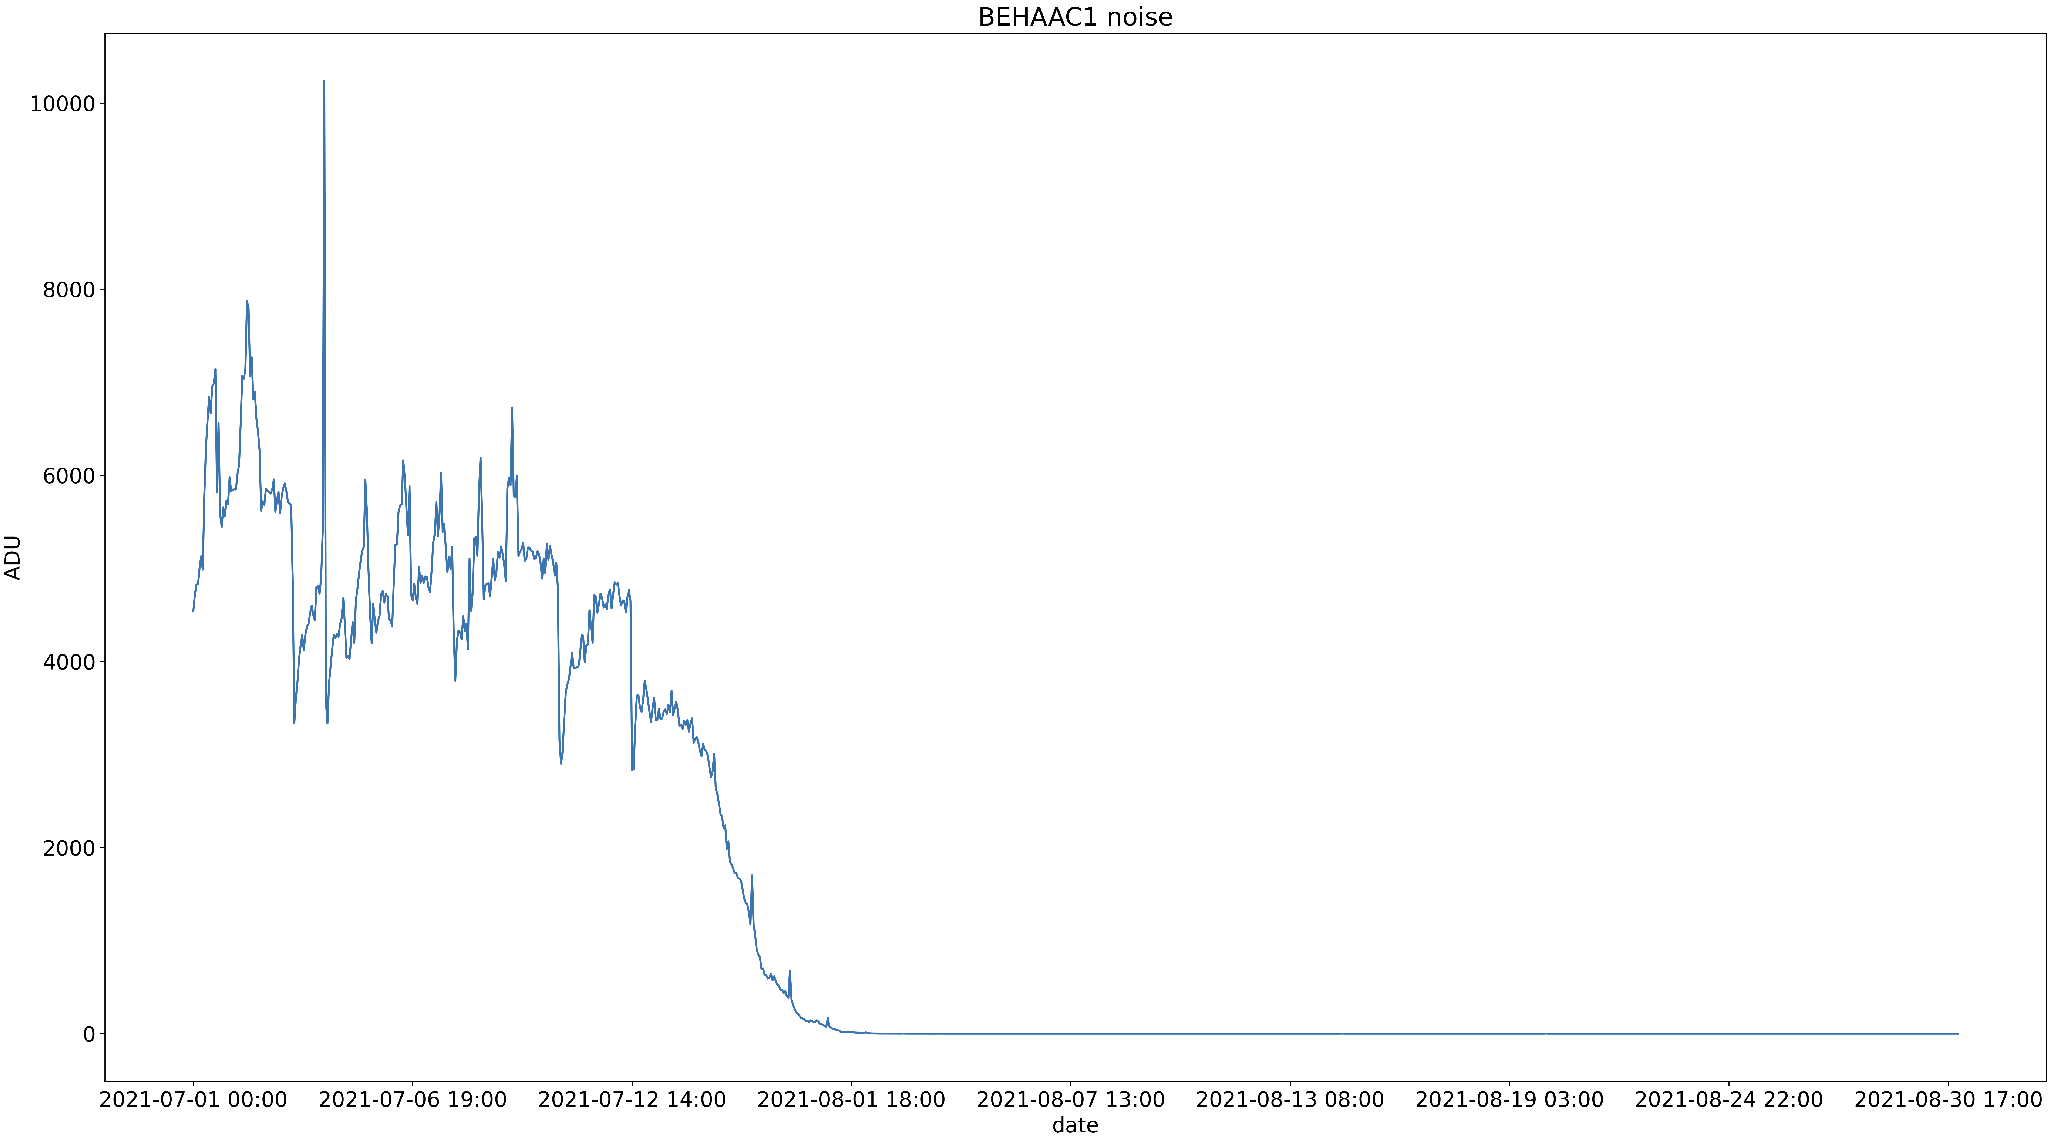
\includegraphics[scale=0.17]{BEHAAC1_2021-07-01_2021-08-31_noise.png}
        \caption{Intensité du bruit de la station BEHAAC, antenne 1 entre le 1\textsuperscript{er} juillet 2021 et le 31 août 2021.}
        \label{fig:BEHAAC-anomalie}
    \end{center}
\end{figure}

\begin{figure}[t]
    \begin{center}
        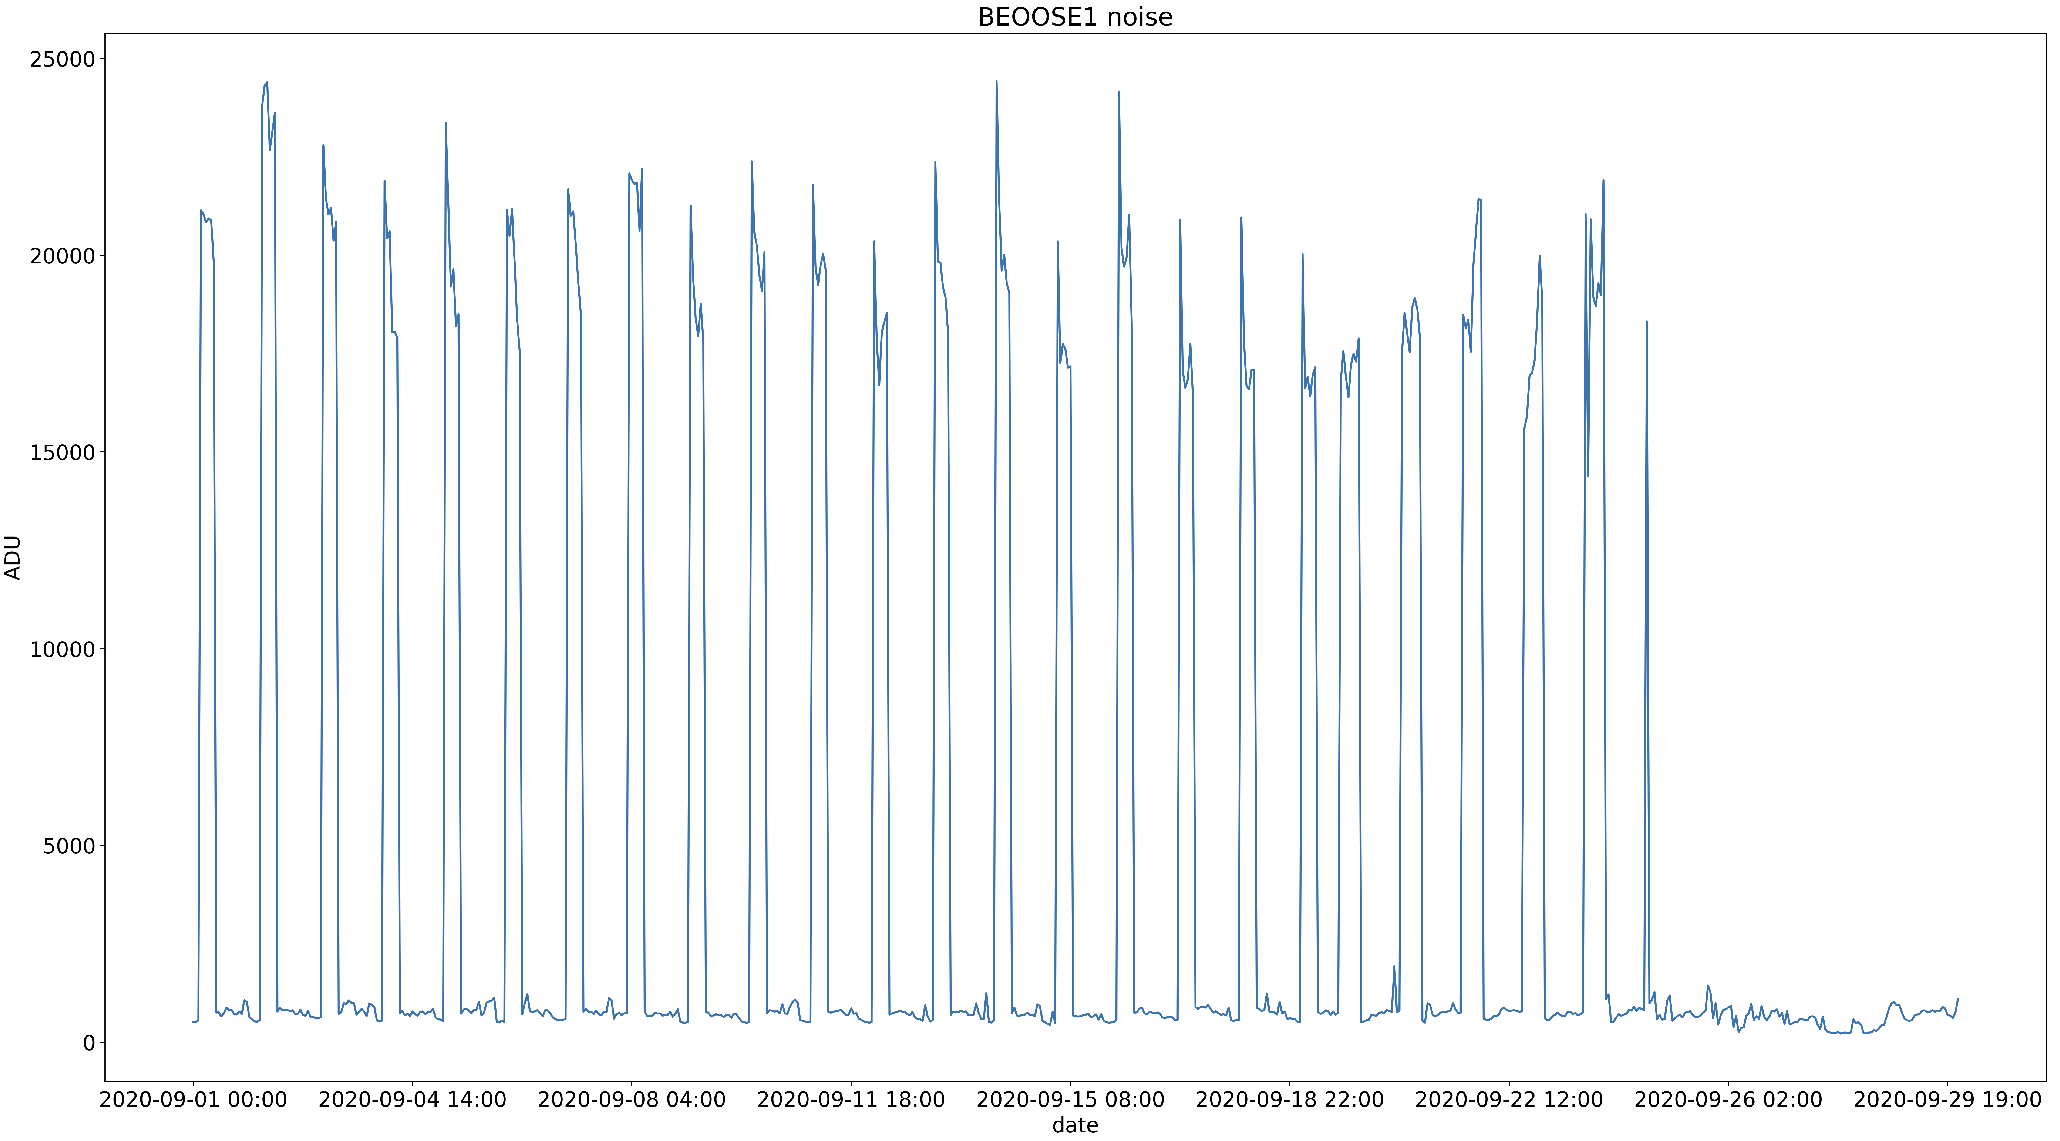
\includegraphics[scale=0.17]{BEOOSE1_2020-09-01_2020-09-30_noise.png}
        \caption{Bruit de la station BEOOSE, antenne 1 entre le 1\textsuperscript{er} septembre 2020 et le 30 septembre 2020.}
        \label{fig:BEOOSE-anomalie}
    \end{center}
\end{figure}

\section{Monitoring des Données BRAMS} \label{sec:monitoring}

Comme évoqué plus haut dans ce rapport, le monitoring des fichiers peut faciliter l'étude des données BRAMS.
Le développement d'un bon logiciel de surveillance relève plusieurs défis.
Il doit être cohérent, et ceci pour tous les types de stations.
De plus, sachant que par jour une grande quantité de fichiers est produit par chaque station, l'optimisation du logiciel est également un facteur important afin de réduire l'utilisation des ressources système et le temps nécessaire pour obtenir les résultats du monitoring.
Dans cette section, le développement du logiciel de surveillance ainsi que les démarches prises afin de résoudre ces défis seront expliqués.

\subsection{Détecter une anomalie sur une station}

Afin de déterminer si un fichier contient une anomalie ou non, il est essentiel de bien choisir les éléments à surveiller.
Dans les sections qui suivent, les différents éléments surveillés dans chaque fichier ainsi que leur pertinence seront expliqués.

\subsubsection{Le Bruit}

L'intensité du bruit est le premier élément qui sera surveillé.
Bien que celui-ci puisse varier légèrement avec le temps, elle devrait rester constante sur une longue période et les grosses variations de bruit sont souvent signe que la station est défectueuse.\\
\\
Ceci était le cas par exemple pour la station BEHAAC lors du mois de juillet 2021.
Comme on peut le voir sur la figure \ref{fig:BEHAAC-anomalie}, on constate une diminution graduelle puis très rapide du bruit.
Ce phénomène, pour les stations v1, est signe que le récepteur ICOM doit être remplacé.
Il faut savoir qu'à partir du moment où le récepteur ne capte presque plus rien, jusqu'à la solution du problème, les données produites par la station sont inutilisables.\\
\\
Un autre exemple de grosses variations de bruit est la station de BEOOSE entre le 1er septembre 2020 jusqu'au 30 septembre 2020.
Quand on visualise la figure \ref{fig:BEOOSE-anomalie}, on remarque de nombreux pics d'intensité du bruit.
La cause de ce problème peut varier au cas par cas, il peut être un mauvais branchement au niveau de la station, des câbles endommagés ou encore un parasite extérieur à la station réceptrice.
Il est important de détecter et résoudre ce problème rapidement puisque le bruit est tellement haut qu'il est impossible de détecter autre chose dans le fichier.\\
\\
Une autre raison de surveiller le bruit est qu'il doit être présent dans chaque fichier.
Un fichier avec un bruit nul est impossible et veut dire qu'au moment où la station a généré le fichier, il avait un problème.
L'intensité du bruit est donc non-seulement une valeur facile à surveiller, mais elle permet également de détecter toute une série de problèmes qui sont de nature différente.

\subsubsection{Le Signal Calibreur}

\begin{figure}[t]
    \begin{center}
        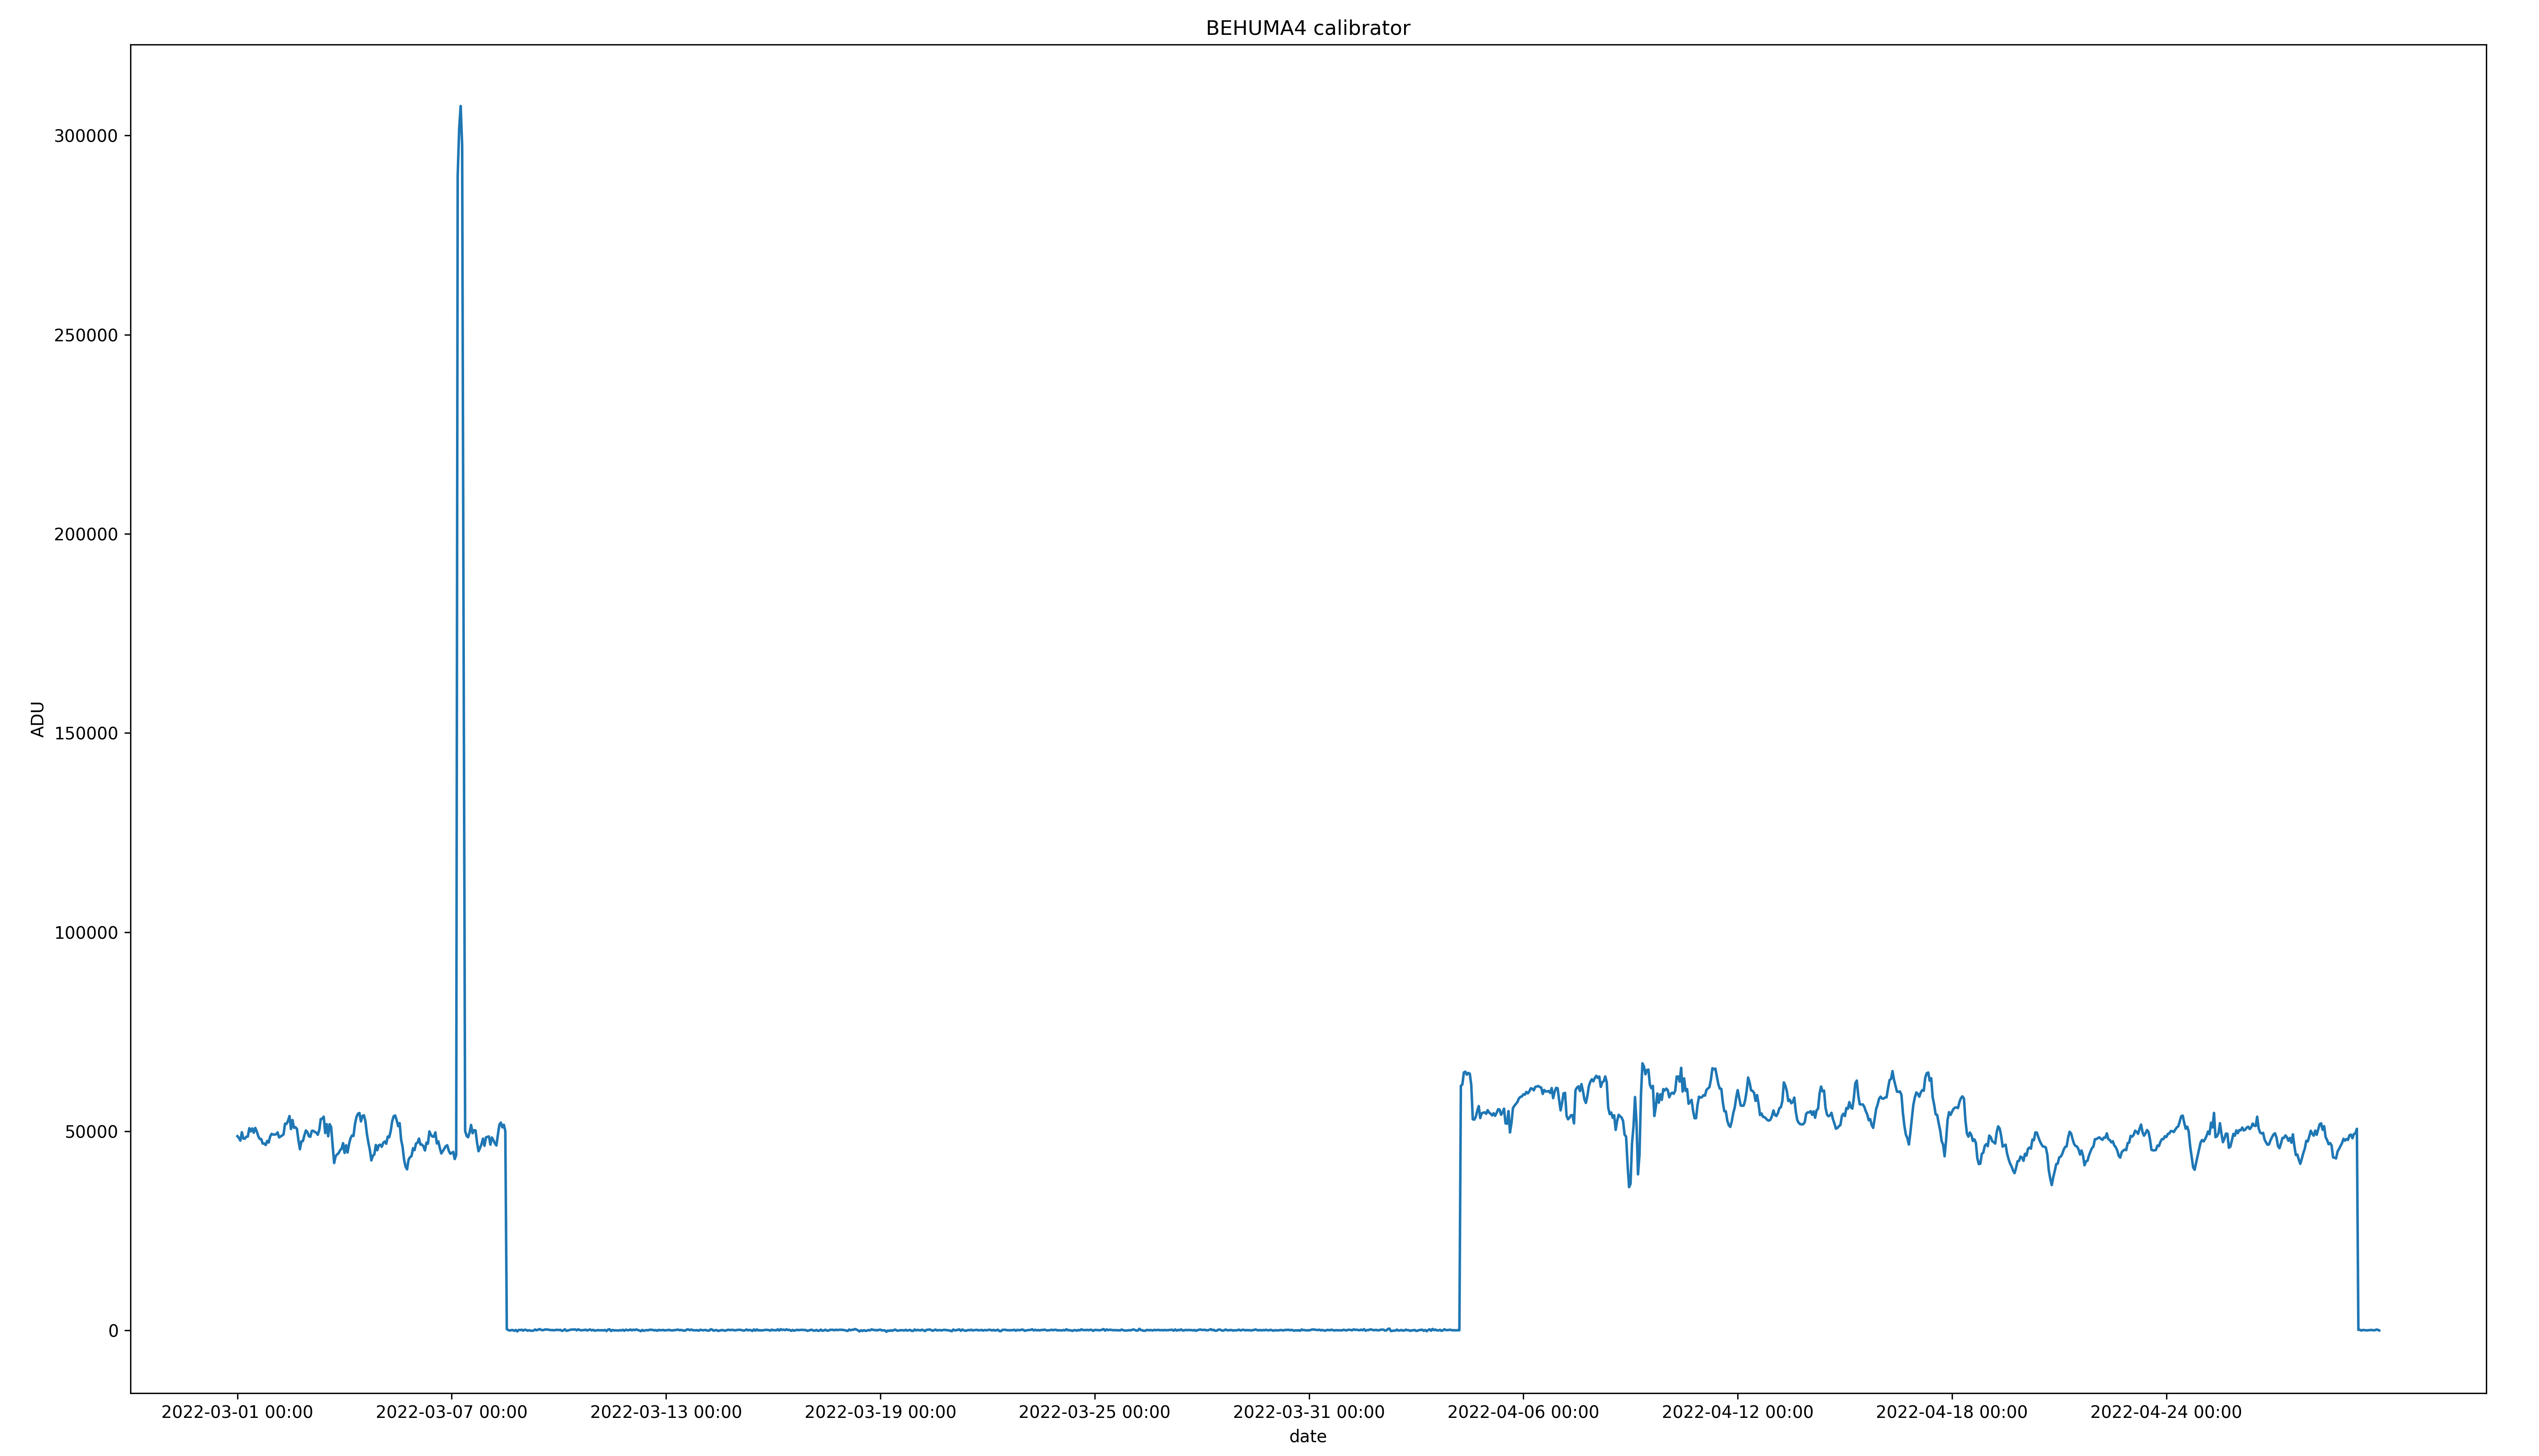
\includegraphics[scale=0.17]{BEHUMA4_2022-03-01_2022-04-30_calibrator.png}
        \caption{Signal calibreur de la station BEHUMA, antenne 4 entre le 1\textsuperscript{er} mars 2022 et le 30 avril 2022.}
        \label{fig:BEHUMA1-anomalie}
    \end{center}
\end{figure}

Le second élément que le programme surveille est l'intensité du signal calibreur ainsi que la fréquence à laquelle celle-ci se trouve.
Mesurer l'intensité de ce signal permet, comme la mesure du bruit, de détecter si un récepteur de la station v1 est cassé.
De plus, comme le bruit, le signal calibreur est un élément qui est censé être présent dans chaque fichier produit par une station réceptrice, s'il est absent cela signifie que la station a un problème ce qui nécessite donc d'être détecté.\\
\\
Vient ensuite la surveillance de la fréquence à laquelle se trouve le signal calibreur.
En théorie, il devrait toujours se trouver à 1500 Hz ; en pratique cette valeur peut varier en particulier avec les anciennes stations où il peut y avoir une translation de fréquence en fonction de la chaleur.
Une variation de cette fréquence entre les valeurs de 1350 Hz et 1750 Hz ne pose pas un grand problème et ne doit donc pas être détectée.
Par contre, une trop grosse variation indique que la station a un défaut, et selon l'anomalie peut rendre les données inutiles.
C'était notamment le cas pour la station BEHUMA4, lors d'une période qui a commencé le 8 mars 2022 et qui s'est étendu jusqu'au 3 avril 2022.
Pendant ce temps, toutes les fréquences étaient décalées d'environ 1000 Hz vers le bas dans chaque fichier généré.
Ceci peut être visualisé à la figure \ref{fig:BEHUMA1-anomalie}.
Bien que ça ne pose pas vraiment de soucis pour le signal calibreur même, qui se trouve alors à environ 500 Hz, toutes les données utiles qu'on retrouve typiquement autour de 1000 Hz se situent maintenant autour de 0 Hz.
Sachant qu'en plus les fréquences basses sont filtrés dans les fichiers BRAMS, l'information utile est donc absente.\\
\\
Le signal calibreur est donc également un élément, se trouvant dans chaque fichier, qui peut indiquer rapidement s'il y a un problème avec une station.
Ensemble avec le bruit, ils forment une bonne base pour déterminer si les données générées sont utilisables et si une station a besoin d'une intervention où non.

\subsection{Fonctionnement du Logiciel de Surveillance}

Ensemble avec les scientifiques du projet BRAMS, nous avons décidé que le programme doit se lancer automatiquement après chaque archivage de données.
Le programme se lance en ligne de commande et ne nécessite aucun paramètre pour fonctionner.
Une fois que le programme est démarré, il va chercher un par un les fichiers WAV nécessaires dans l'archive BRAMS.
Dans le but d'avoir une surveillance suffisante sans utiliser trop de ressources machines, nous avons décidés d'analyser un fichier par heure par station.
Ceci revient à l'analyse de 24 fichiers par jour par station.

\subsubsection{Analyse des Fichiers WAV}
%! image with detection zones

\begin{figure}
    \begin{lstlisting}[style=CStyle]
def get_psd(f, flow=800, fhigh=900):
    # get fourier tranform from BramsWavFile class
    freq, S, fbin = f.FFT(f.Isamples)
    idx = (freq >= flow) * (freq < fhigh)

    # calculate the total power of the wanted frequencies
    p = (S[idx] * S[idx].conj()).real / 2

    # get a mean normalized to 1Hz
    psd = p.mean() / fbin

    return psd
    \end{lstlisting}
    \caption{Code de la fonction permettant de calculer la dsp.}
    \label{fig:psd-code}
\end{figure}

Pour chercher et lire un fichier WAV provenant d'une station réceptrice, le logiciel utilise une classe nommée BramsWavFile.
La base de cette classe a été écrite par Michel Anciaux.
Cependant, ce code a subi deux grandes modifications afin de l'adapter pour le programme de monitoring et pour le rendre plus modulable.
Le premier grand changement implique la recherche des fichiers dans l'archive : tandis que le code non modifié nécessitait un chemin pour trouver le fichier, maintenant il est capable de chercher tout seul un fichier dans l'archive BRAMS ou dans un autre dossier sur base de quelques informations (date et heure du fichier, station, numéro d'antenne).
Le second changement concerne l'optimisation et donc le temps nécessaire pour lire un fichier WAV.
Toutes les étapes non nécessaires ont été effacées et plusieurs librairies ont été testées afin de trouver celle qui était la plus rapide.
Pour la méthode FFT de la classe BramsWavFile, qui permet de calculer la transformée de Fourier d'un fichier WAV, la librairie Scipy offrait par exemple des performances supérieures à la librairie Numpy tout en offrant les mêmes fonctionnalités et la même portabilité.\\
\\
Une fois les valeurs du fichier WAV obtenues, on calcule d'abord la densité spectrale de puissance (dsp) du bruit.
La dsp représente la répartition des puissances en fonction des différentes fréquences contenues dans un signal.
L'unité de la dsp est exprimé en puissance par Hertz.\\
\\
Afin d'avoir une estimation précise du bruit sans devoir calculer la dsp de tout le bruit dans un fichier, on prend uniquement la dsp entre 800 Hz et 900 Hz.
Entre ces deux fréquences on ne trouve normalement pas d'éléments autres que le bruit.
Dans un cas contraire, c'est souvent une indication qu'il y a un problème avec une station.
Le code permettant de calculer la dsp du bruit est affiché à la figure \ref{fig:psd-code}.
Dans un premier temps, on calcule la FFT du fichier WAV.
Ce calcul nous donne trois variables : une liste avec les valeurs de l'axe x (freq), un vecteur avec les valeurs de l'axe y (S) en fonction de l'axe x et la résolution fréquentielle de l'axe x (fbin).
Ensuite, on calcule le spectre des puissances en multipliant le vecteur S par son conjugué, ce qui nous donne son carré et donc la puissance pour chaque fréquence de l'axe x.
Enfin, on fait la moyenne de ce vecteur et on divise cette moyenne par la résolution fréquentielle ce qui nous donne une moyenne par Hz du bruit et donc la dsp.\\
\\
Après, le programme passe à la recherche de la fréquence du signal calibreur.
Il fait ceci en recherchant l'intensité maximale entre les fréquences de 1350 Hz et 1750 Hz dans un fichier.
Comme le signal calibreur s'étend sur l'entièreté de la durée du fichier, il doit toujours avoir la valeur maximale entre ces deux fréquences.
La fréquence retrouvée nous permet alors de calculer la dsp du signal.
Il y a ici deux différences par rapport au calcul de la dsp du bruit.
La première concerne la bande de fréquence utilisée pour le calcul : pour le signal calibreur, elle est calculée sur une bande de 10 Hz autour de la fréquence trouvée pour cette dernière.
La deuxième différence implique la soustraction de la dsp du bruit une fois la dsp du signal calibreur obtenue.
Cette étape est faite afin de disposer d'une estimation plus précise.\\
\\
Les étapes listées ci-dessus permettent d'avoir les informations nécessaires afin de pouvoir déterminer s'il y a un problème avec un fichier, et donc par conséquence, avec une station.
Les deux valeurs de dsp sont enregistrées dans la base de données du projet BRAMS et sont donc réutilisables.

% TODO
\subsubsection{L'avertissement d'une anomalie}

\begin{figure}
    \begin{lstlisting}[style=CStyle]
def detect_variations(y_data, current_value):
    q1 = np.percentile(y_data, 25, interpolation='lower')
    q3 = np.percentile(y_data, 75, interpolation='higher')

    interquartile = q3 - q1

    upper_limit = q3 + (2.4 * interquartile)
    lower_limit = q1 - (2.4 * interquartile)

    if current_value >= upper_limit:
        return 1
    elif current_value <= lower_limit:
        return -1
    else:
        return 0
    \end{lstlisting}
    \caption{Code de la fonction permettant de détecter des variations excessives dans les données.}
    \label{fig:detection-code}
\end{figure}

Avant l'enregistrement, une autre étape est complétée : la détection automatique d'une anomalie.
Pour cette étape, le logiciel applique les mêmes actions sur le bruit et le signal calibreur avec une exception, qui sera expliquée plus bas dans cette section.
Ces actions sont répétées à chaque fois qu'une nouvelle valeur de dsp est générée.\\
\\
Afin de détecter une grande variation dans les données, le programme se base sur l'ensemble des valeurs de dsp des deux semaines précédent la nouvelle valeur de dsp.
À partir de cet ensemble, il faut définir une frontière haute et une frontière basse.
Si la nouvelle dsp se trouve en dehors d'une frontière, il sera considéré comme anormal et les scientifiques du projet BRAMS seront avertis.\\
\\
Différentes méthodes existent pour définir ces frontières.
La méthode utilisée dans ce logiciel, utilisant la gamme interquartile, peut être visualisée à la figure \ref{fig:detection-code} et est expliquée ci-dessous.\\
\\
Il faut savoir que les deux paramètres de la fonction affichée à la figure \ref{fig:detection-code}, \textbf{y\_data} et \textbf{current\_value}, sont l'ensemble des valeurs de dsp des deux semaines précédent la nouvelle valeur de dsp et la nouvelle valeur de dsp même.
%! exposant chars
Le programme commence par calculer le 25e et le 75e percentile de l'ensemble des données qui se trouvent dans y\_data.
Un percentile est une mesure indiquant la valeur en dessous de laquelle se trouvent un pourcentage donné d'observations, dans un ensemble d'observations.
Par exemple, le 20e percentile est la valeur en dessous de laquelle se trouvent 20\% des observations dans un ensemble d'observations.
Ensuite, on calcule la gamme interquartile de y\_data.
Cette valeur est calculée en faisant la différence entre la 25e et la 75e percentile, que le programme a déjà calculé.\\
\\
Le logiciel définira à partir de ces trois valeurs calculées, la frontière haute et basse.
Les formules utilisées sont \(Q3 + (x * IQR)\) pour la frontière haute et \(Q1 - (x * IQR)\) pour la frontière basse où \(Q1\) et \(Q3\) sont le 25e et le 75e percentile et \(IQR\) la gamme interquartile.
Le facteur \(x\) permet de définir la largeur entre les deux frontières, au plus sa valeur est élevée, au plus les frontières sont écartées.\\
\\
C'est ce facteur qui est différent pour le bruit et le signal calibreur.
Tandis que pour le bruit, il vaut 2.4, il est défini à  2.5 pour le signal du calibreur.
La différence entre ces valeurs est que le bruit varie moins et il n'est donc pas nécessaire d'avoir les deux frontières aussi écartées que pour le signal du calibreur.\\
\\
Finalement, on vérifie si la nouvelle valeur de dsp (\textbf{current\_value}) dépasse ou non une des frontières.
Si c'est le cas, on informe l'utilisateur d'un problème dans les données.\\
\\
Bien que cette méthode permet bien de détecter des anomalies, elle n'est pas parfaite.
En effet, parfois il y a des faux positifs et le programme alerte l'utilisateur alors qu'aucun problème est présent.

\subsection{L'interface sur le site web BRAMS}

%! lower both figures
\begin{figure}[t]
    \begin{center}
        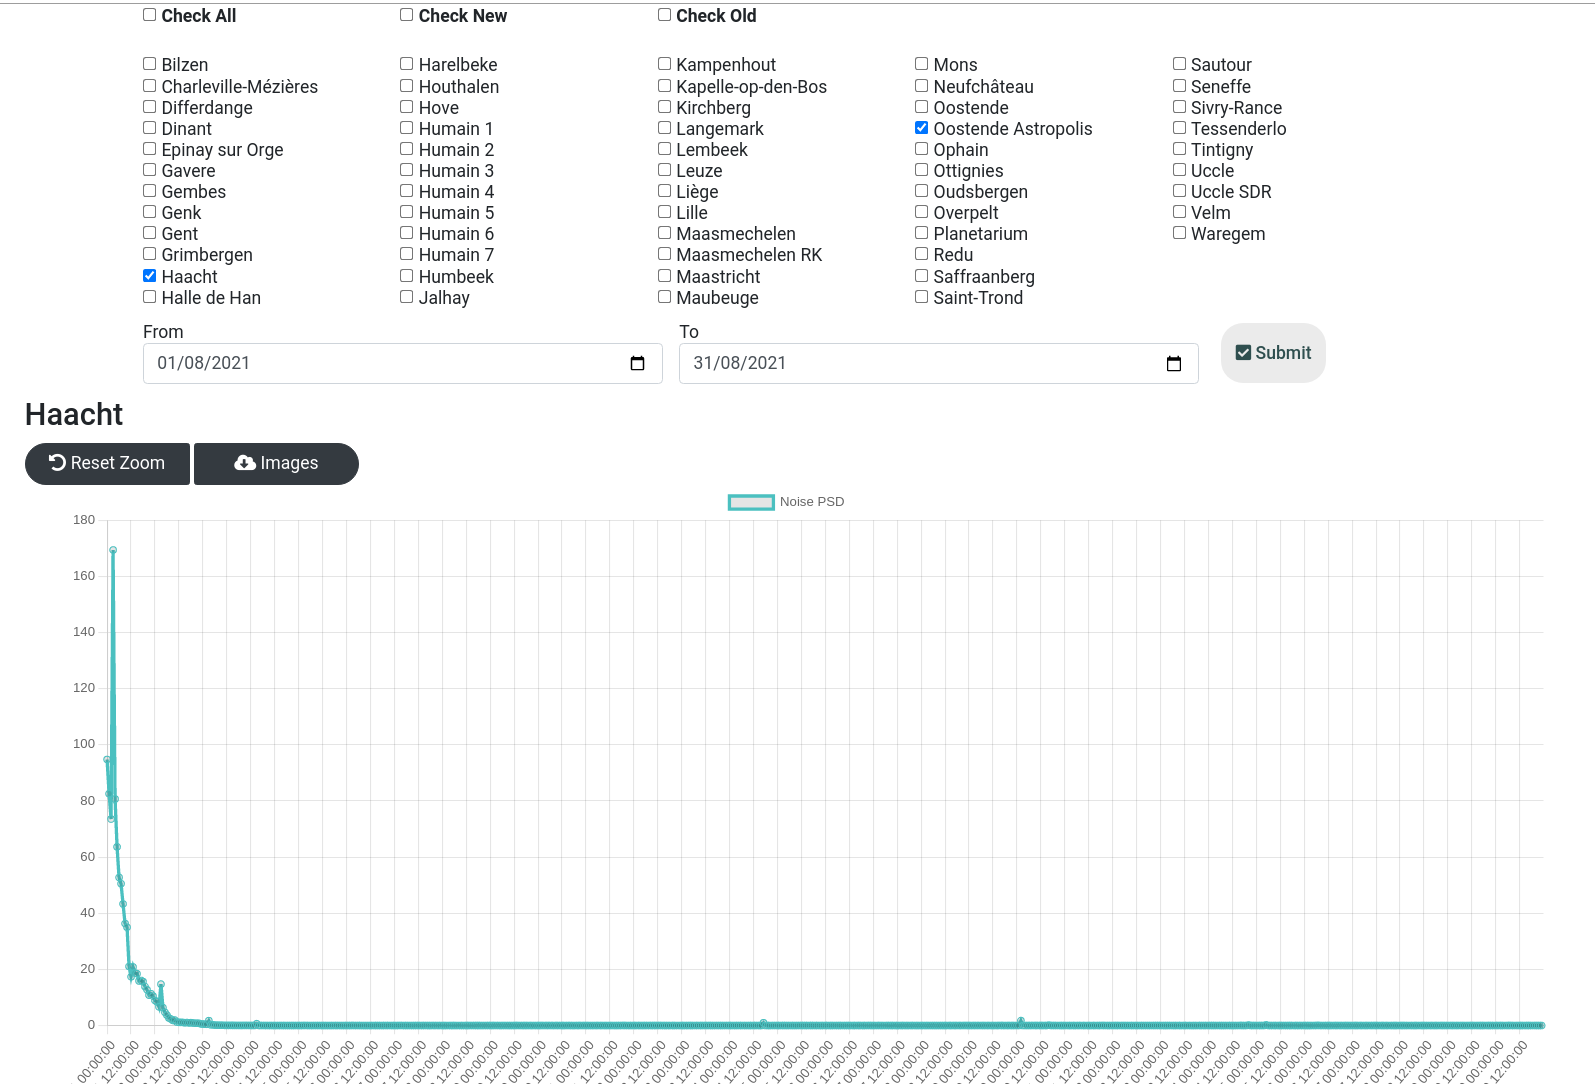
\includegraphics[scale=0.22]{monitoring_ui.png}
        \caption{Interface graphique du logiciel de surveillance.}
        \label{fig:monitoring-ui}
    \end{center}
\end{figure}

\begin{figure}[t]
    \begin{center}
        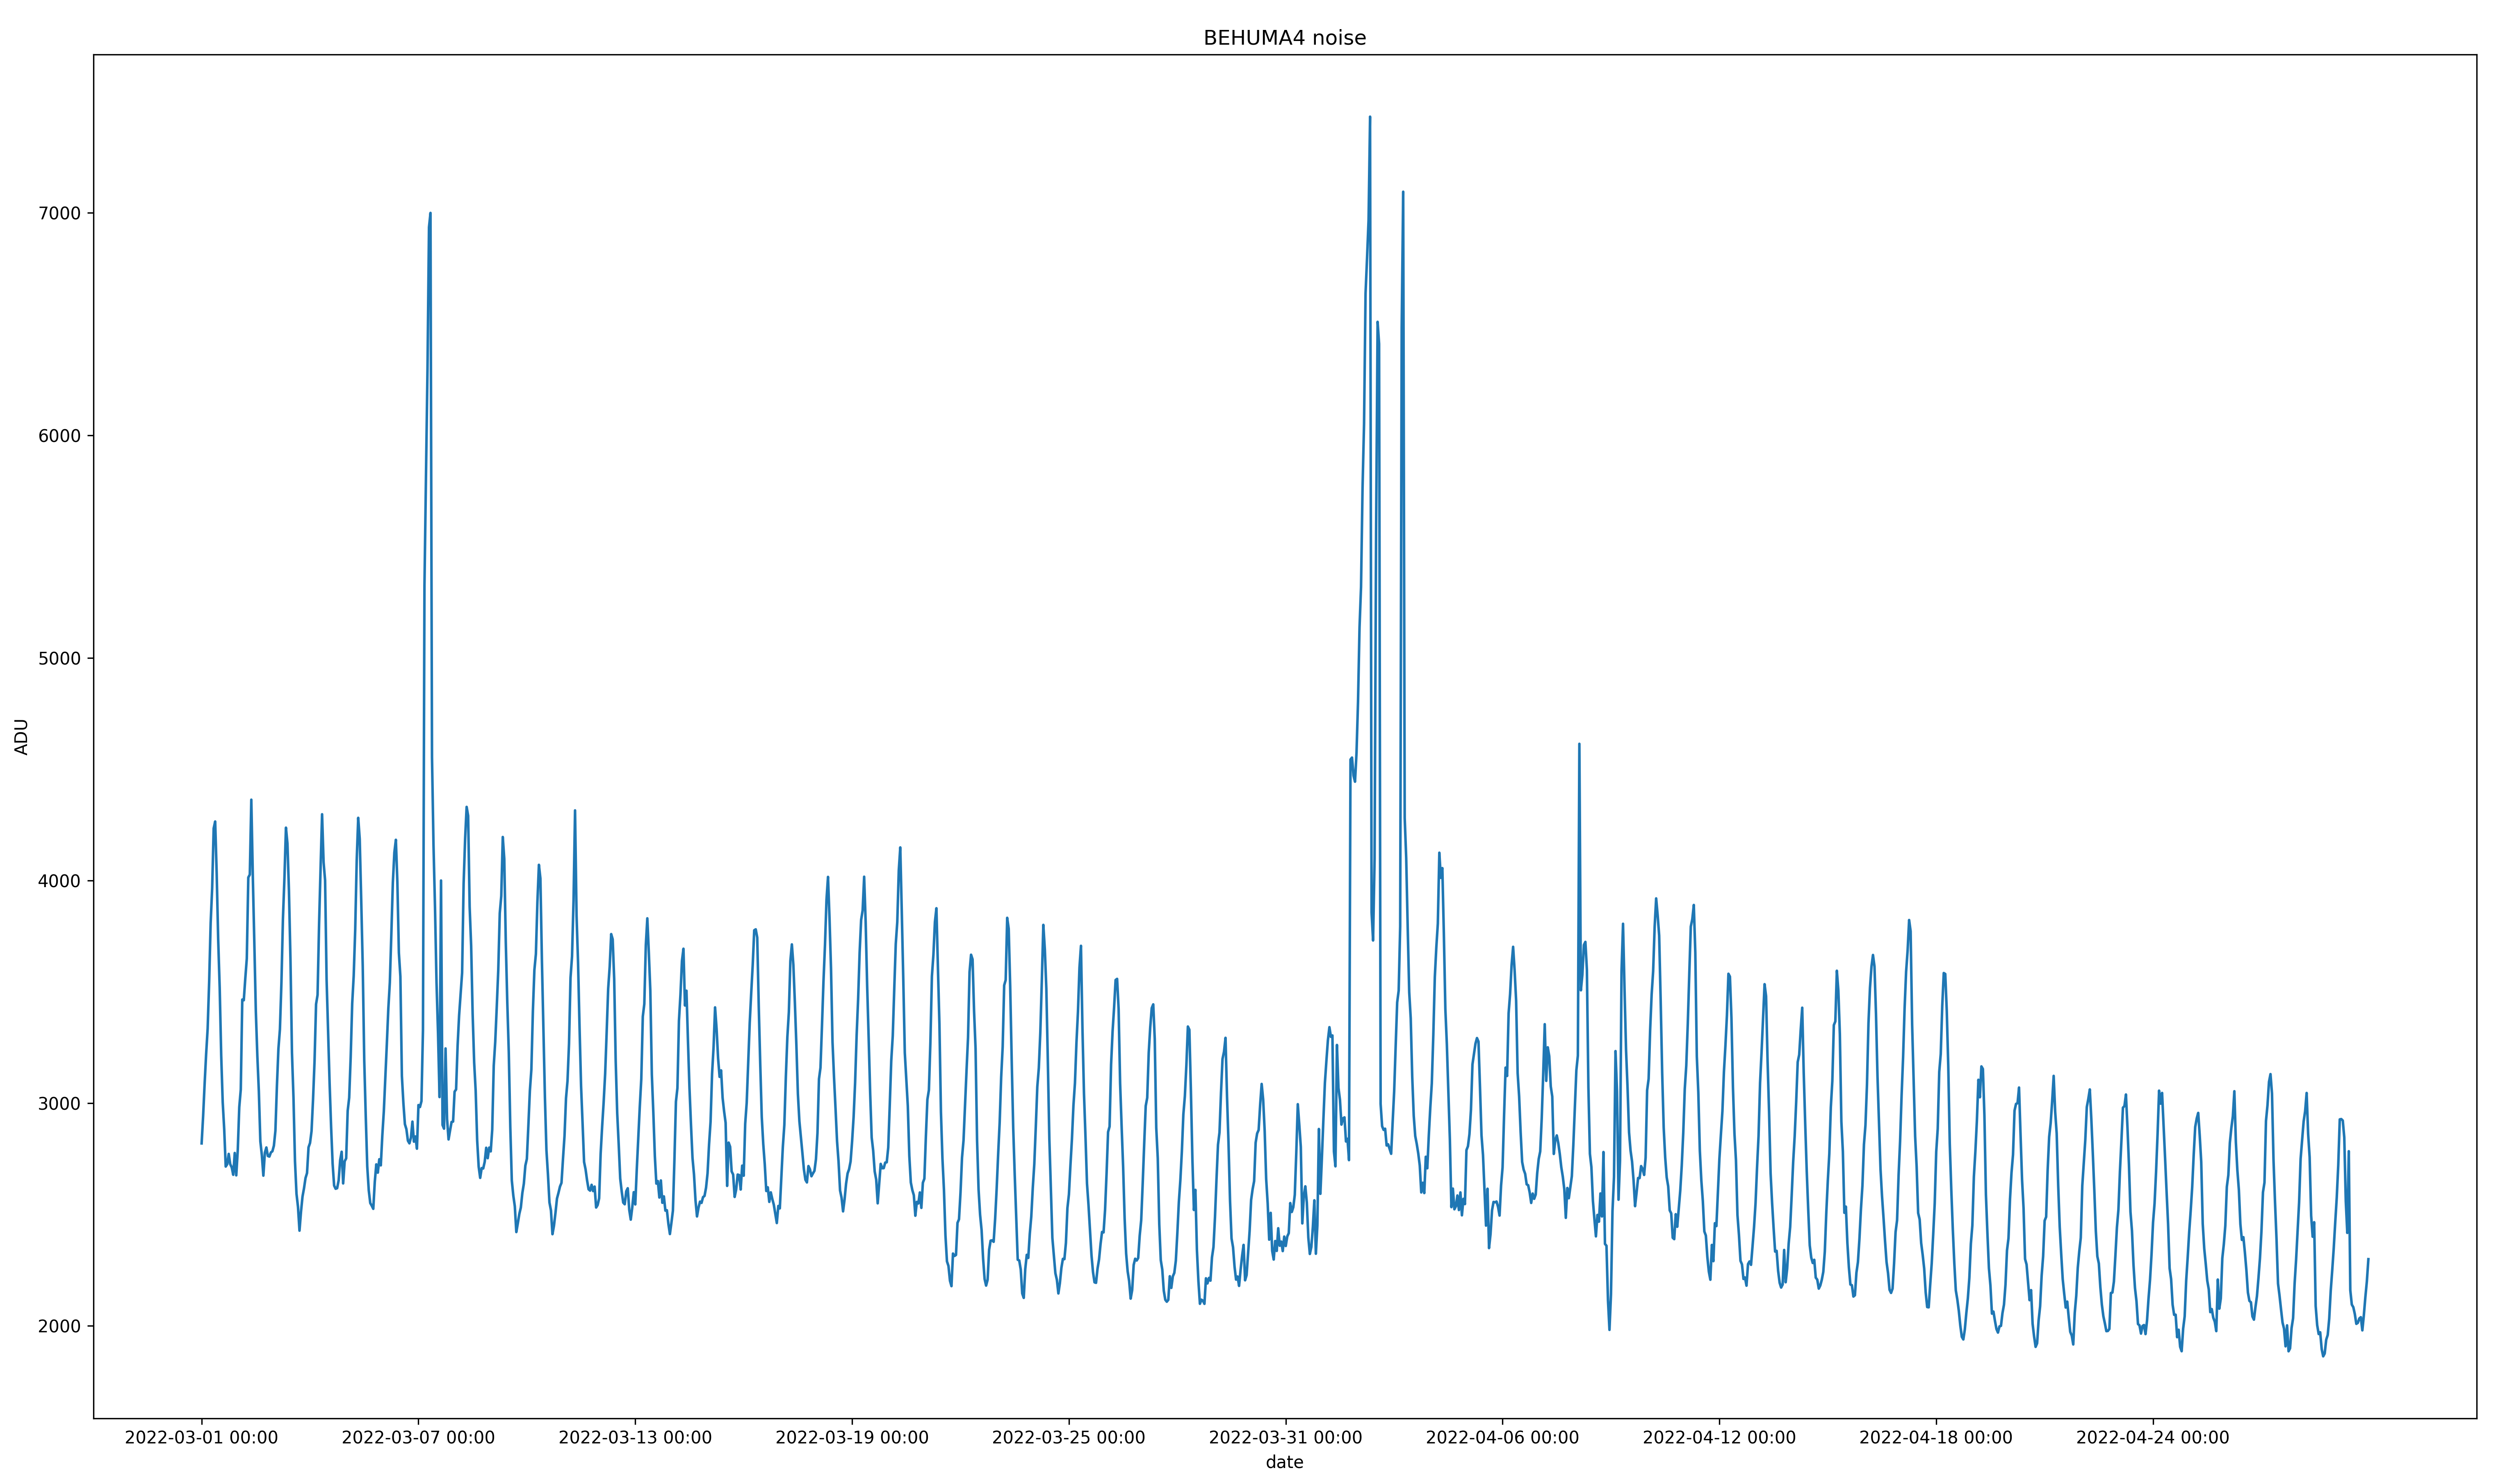
\includegraphics[scale=0.17]{BEHUMA4_2022-03-01_2022-04-30_noise.png}
        \caption{Signal du bruit de la station BEHUMA, antenne 4 entre le 1\textsuperscript{er} mars 2022 et le 30 avril 2022.}
        \label{fig:BEHUMA4-variations}
    \end{center}
\end{figure}

En plus de la détection automatique d'une anomalie, une interface graphique permettant de visualiser l'évolution de la dsp du signal calibreur et du bruit a été développée.
Il faut noter que cette interface est indépendante du programme de monitoring même, elle utilise, cependant, les données générées par ce-dernier.
Comme on peut le voir sur la figure  \ref{fig:monitoring-ui}, l'interface affiche deux graphiques pour chaque station que l'utilisateur a sélectionnée.
Le premier représente les valeurs de dsp pour le bruit, pour une période que l'utilisateur a indiquée et le deuxième affiche la même chose, mais cette fois-ci pour le signal calibreur.\\
\\
Cette interface permet aux scientifiques du projet BRAMS de surveiller ces valeurs et éventuellement de détecter un problème qui ne serait pas détecté par la surveillance automatique.
De plus, elle donne la possibilité de mieux comprendre les variations en observant des motifs qui reviennent.
Un des motifs retrouvés lors des tests est une diminution de la dsp du bruit lorsque la nuit approche.
Ceci est particulièrement visible sur la figure \ref{fig:BEHUMA4-variations} qui représente la dsp du bruit pour la station BEHUMA4 du 1er mars 2022 au 30 avril 2022.\\
\\
Cette interface graphique, comme l'entièreté du nouveau site web BRAMS utilise Joomla comme back-end.
Joomla est un framework gratuit et open-source utilisant le langage PHP.
Pour afficher les différents graphiques, le front-end de l'interface utilise la librairie JavaScript open-source ChartJS\footnote{https://www.chartjs.org/}.
Cette librairie permet d'afficher des beaux graphiques et de les agrandir si nécessaire.
Cette interface sera disponible publiquement sur le nouveau site web BRAMS dès le déploiement de cette dernière.
Plus d'images de cette interface sont disponibles à l'annexe \ref{app:monitoring-ui}.

\newpage

\section{Logiciel de Détection des Météores}

Une fois que les données sont archivées, les membres du projet BRAMS commencent à les analyser et les interpréter.
Un objectif assez important de ce projet est le calcul de la trajectoire d'un météore dans l'atmosphère.
Pour retrouver la trajectoire d'un météore à l'aide du réseau BRAMS, il faut qu'un météore soit détecté par au moins huit stations réceptrices.
Vérifier manuellement, pour chaque station, si celle-ci a détecté un météore est une tâche prenant un temps non négligeable.
Dans cette section, le développement d'un programme permettant de réduire la perte de temps causée par cette procédure est expliquée.
Ce programme est entièrement indépendant du programme de monitoring, expliqué dans la section \ref{sec:monitoring}.

\subsection{Déterminer si un Écho Appartient à un Météore}

Avant de développer un logiciel, il est nécessaire de savoir comment trouver, sur différentes stations réceptrices, les échos venant d'un seul météore.
Différents facteurs peuvent indiquer qu'un écho vient d'un météore spécifique ou non.
Parmi les facteurs connus on trouve l'emplacement de la station qui a détecté l'écho de météore et le moment où l'écho est détecté.
Dans le cas de ce logiciel, le facteur temps sera utilisé.\\
\\
Quand on compare plusieurs échos de météores, tous détectés par des stations différentes, le facteur temps permet de donner une idée s'ils proviennent du même météore ou non.
En effet, par expérience on sait que lorsqu'un météore est détecté par plusieurs stations, toutes ces détections se font dans un intervalle d'environ trois secondes.
Bien que ce facteur ne permet pas d'assurer complètement qu'un écho vient d'un météore spécifique, il permet d'éliminer toutes les stations où aucun écho n'a été détecté pour un météore, réduisant grandement le temps nécessaire pour les scientifiques du projet BRAMS.
De plus, si dans l'intervalle recherché on ne trouve qu'un écho, ceci augmente fortement les chances que celui-ci appartient au météore recherché.

\begin{figure}[htp]
    \begin{center}
        \includegraphics[scale=0.13]{original_spectro.png}
        \caption{Spectrogramme original de la station BEHUMA 1 le 23 avril 2022 à 00h00}
        \label{fig:spectro-orig}
    \end{center}
\end{figure}

\begin{figure}[hbp]
    \begin{center}
        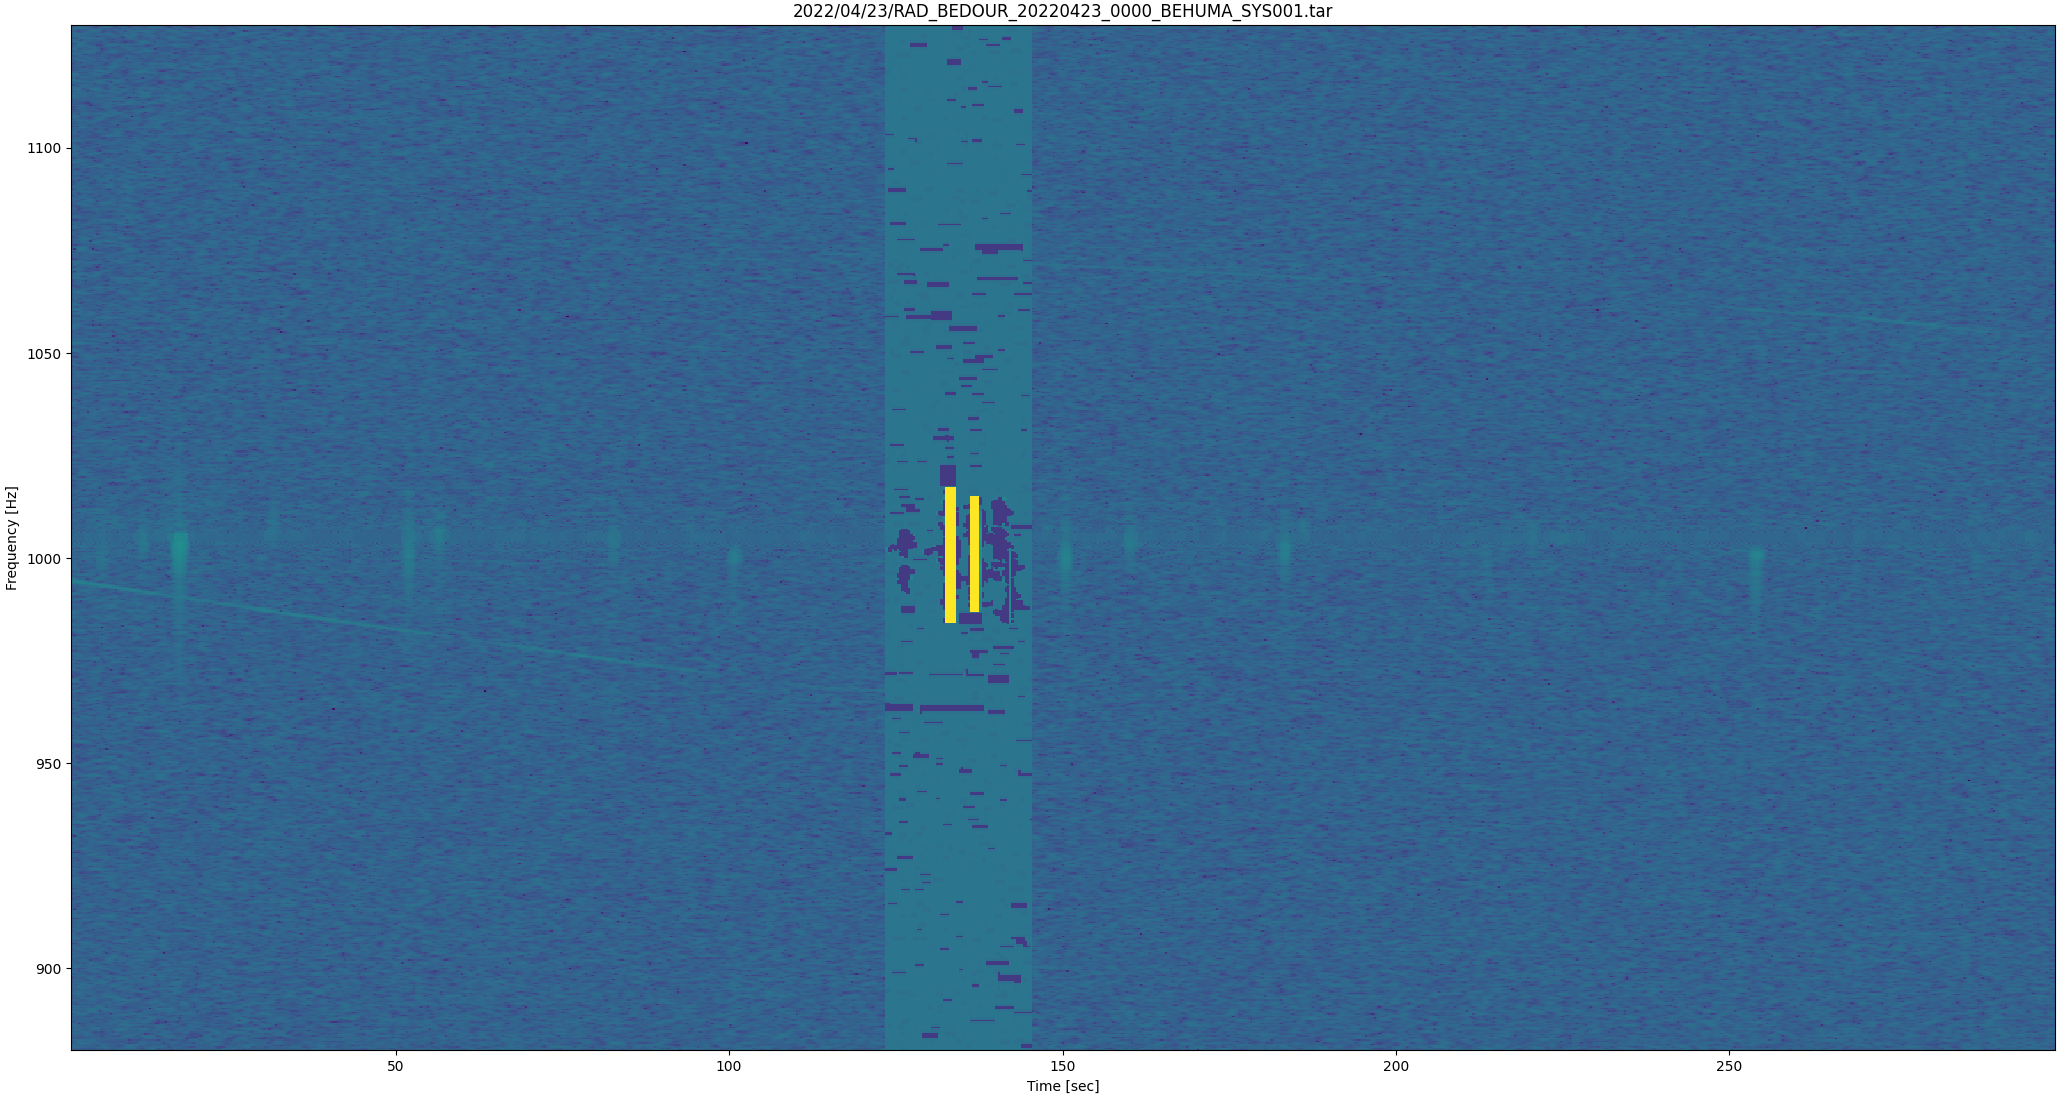
\includegraphics[scale=0.13]{meteor_detect_example.png}
        \caption{Résultat du système de détection de météores.}
        \label{fig:meteor-detect-ex}
    \end{center}
\end{figure}

\subsection{Fonctionnement du Logiciel}

Le programme développé se lance en ligne de commande et nécessite un paramètre obligatoire : un temps précis à la seconde, autour duquel on va rechercher d'autres échos.
Un deuxième paramètre optionnel est le code de location d'une station où on est sûr d'avoir détecté le météore recherché.\\
\\
Une fois que le programme est lancé, il calcule l'intervalle.
Si le temps donné en entrée est nommé \(t0\) et que $\Delta$\(t\) vaut trois secondes, l'intervalle calculé vaut \([t0 - \)$\Delta$\(t ; t0 + \)$\Delta$\(t]\).
Le programme va ensuite chercher tous les fichiers contenant cet intervalle.
Afin de compléter cette action, il utilise la classe BramsWavFile qui est également utilisée pour le programme de monitoring.\\
\\
Pour chaque fichier récupéré, il calcule le spectrogramme et détecte les météores présents dans l'intervalle calculé.
La détection des météores, en ce moment, est fait par un code développé en parallèle avec le logiciel expliqué dans cette section.
Cependant, ce code est temporaire et est voué à disparaitre pour une solution plus efficace qui est en cours de développement par les membres du projet BRAMS et utilisant le machine learning.
Actuellement pour détecter les météores, différentes étapes sont exécutées par le code sur le spectrogramme.
Ces étapes sont listées ci-dessous et leur application sera montrée sur base du spectrogram non changé affiché à la figure \ref{fig:spectro-orig}.

\begin{figure}[h]
    \begin{lstlisting}[style=CStyle]
def filter_by_percentile(
    self,
    start=0,
    end=None,
    percentile=95
):
    spectrogram_slice = self.__get_slice(start, end)

    for column in spectrogram_slice.T:
        column_percentile = np.percentile(column, percentile)
        column[column < column_percentile] = 0
    \end{lstlisting}
    \caption{Code permettant d'appliquer le filtre par percentile.}
    \label{fig:percentile-code}
\end{figure}

\begin{enumerate}
    \item L'amplification des objets ressemblants à des météores par un filtre.
          Ce filtre a été développé spécialement pour ce but et peut être visualisé à l'annexe \ref{app:kernel}.
          Le filtre est appliqué à l'aide d'une convolution.
          Une convolution est une opération mathématique qui prend deux fonctions en entrée et qui produit un nouveau signal.
          Dans ce cas-ci, les signaux en entrée sont le spectrogramme, ou une partie du spectrogramme, et le filtre.
          Un résultat de cette convolution sur un spectrogramme est représenté à l'annexe \ref{app:spectro-mod1}.
    \item La suppression du bruit en appliquant un filtre par percentile.
          %! exposant character
          % Ceci implique que pour chaque colonne du spectrogramme dans l'intervalle calculée, le programme va mettre à zéro toutes les cellules dont la valeur est inférieure que la 95e percentile de cette même colonne.
          Cette étape est effectuée par la fonction affichée à la figure \ref{fig:percentile-code}.
          Ce code débute en prenant l'intervalle dans lequel on recherche des échos (ligne 7).
          Une fois cet intervalle récupéré, on calcule pour chaque colonne le 95e percentile.
          Toutes les valeurs de cette colonne inférieures à ce percentile sont ensuite mises à zéro (ligne 9 à 12).
          On peut observer l'effet de ce filtre à l'annexe \ref{app:spectro-mod2}, où l'on voit bien que l'intervalle dans lequel on recherche des échos de météores est bien plus propre qu'à l'annexe \ref{app:spectro-mod1}.
    \item L'élimination de tous les objets qui sont trop petits pour pouvoir être l'écho d'un météore.
          Pour cette étape, une labellisation du spectrogramme est appliquée.
          Une labellisation, dans ce cas, est une action où l'on retrouve tous les objets séparés, non-nuls sur le spectrogramme.
          On vérifie alors leur taille et on les compare à la taille minimale qu'un écho de météore peut avoir.
          Si la taille de l'objet est inférieure à la taille minimale, elle est mise à zéro.
          Ceci peut être visualisé à l'annexe \ref{app:spectro-mod3} où l'on peut observer, dans l'intervalle où on recherche des échos de météores, des tâches bleues.
          Ces tâches bleues sont des éléments qui se sont fait éliminer par cette étape.
    \item La suppression des échos d'avions.
          En effet, les météores ne sont pas les seuls objets qui traversent l'atmosphère et qui sont détectés par les stations réceptrices.
          Les échos d'avions sont des parasites dans les fichiers BRAMS et le programme ne peut pas les confondre avec des échos de météores.
          C'est pour cette raison que le logiciel vérifie, pour chaque objet restant sur le spectrogramme à cette étape, si cet objet n'est pas trop large pour être un météore.
\end{enumerate}

Après toutes ces actions, les objets restants sur le spectrogramme sont considérés comme étant des échos de météores et le programme récupère leurs coordonnées.
Un exemple de résultat final de la détection des météores est affiché à la figure \ref{fig:meteor-detect-ex}.
Notez que cette image n'est pas la sortie du programme et qu'elle ne s'affiche pas lors du déroulement du programme.

%! change image
\begin{figure}[H]
    \begin{center}
        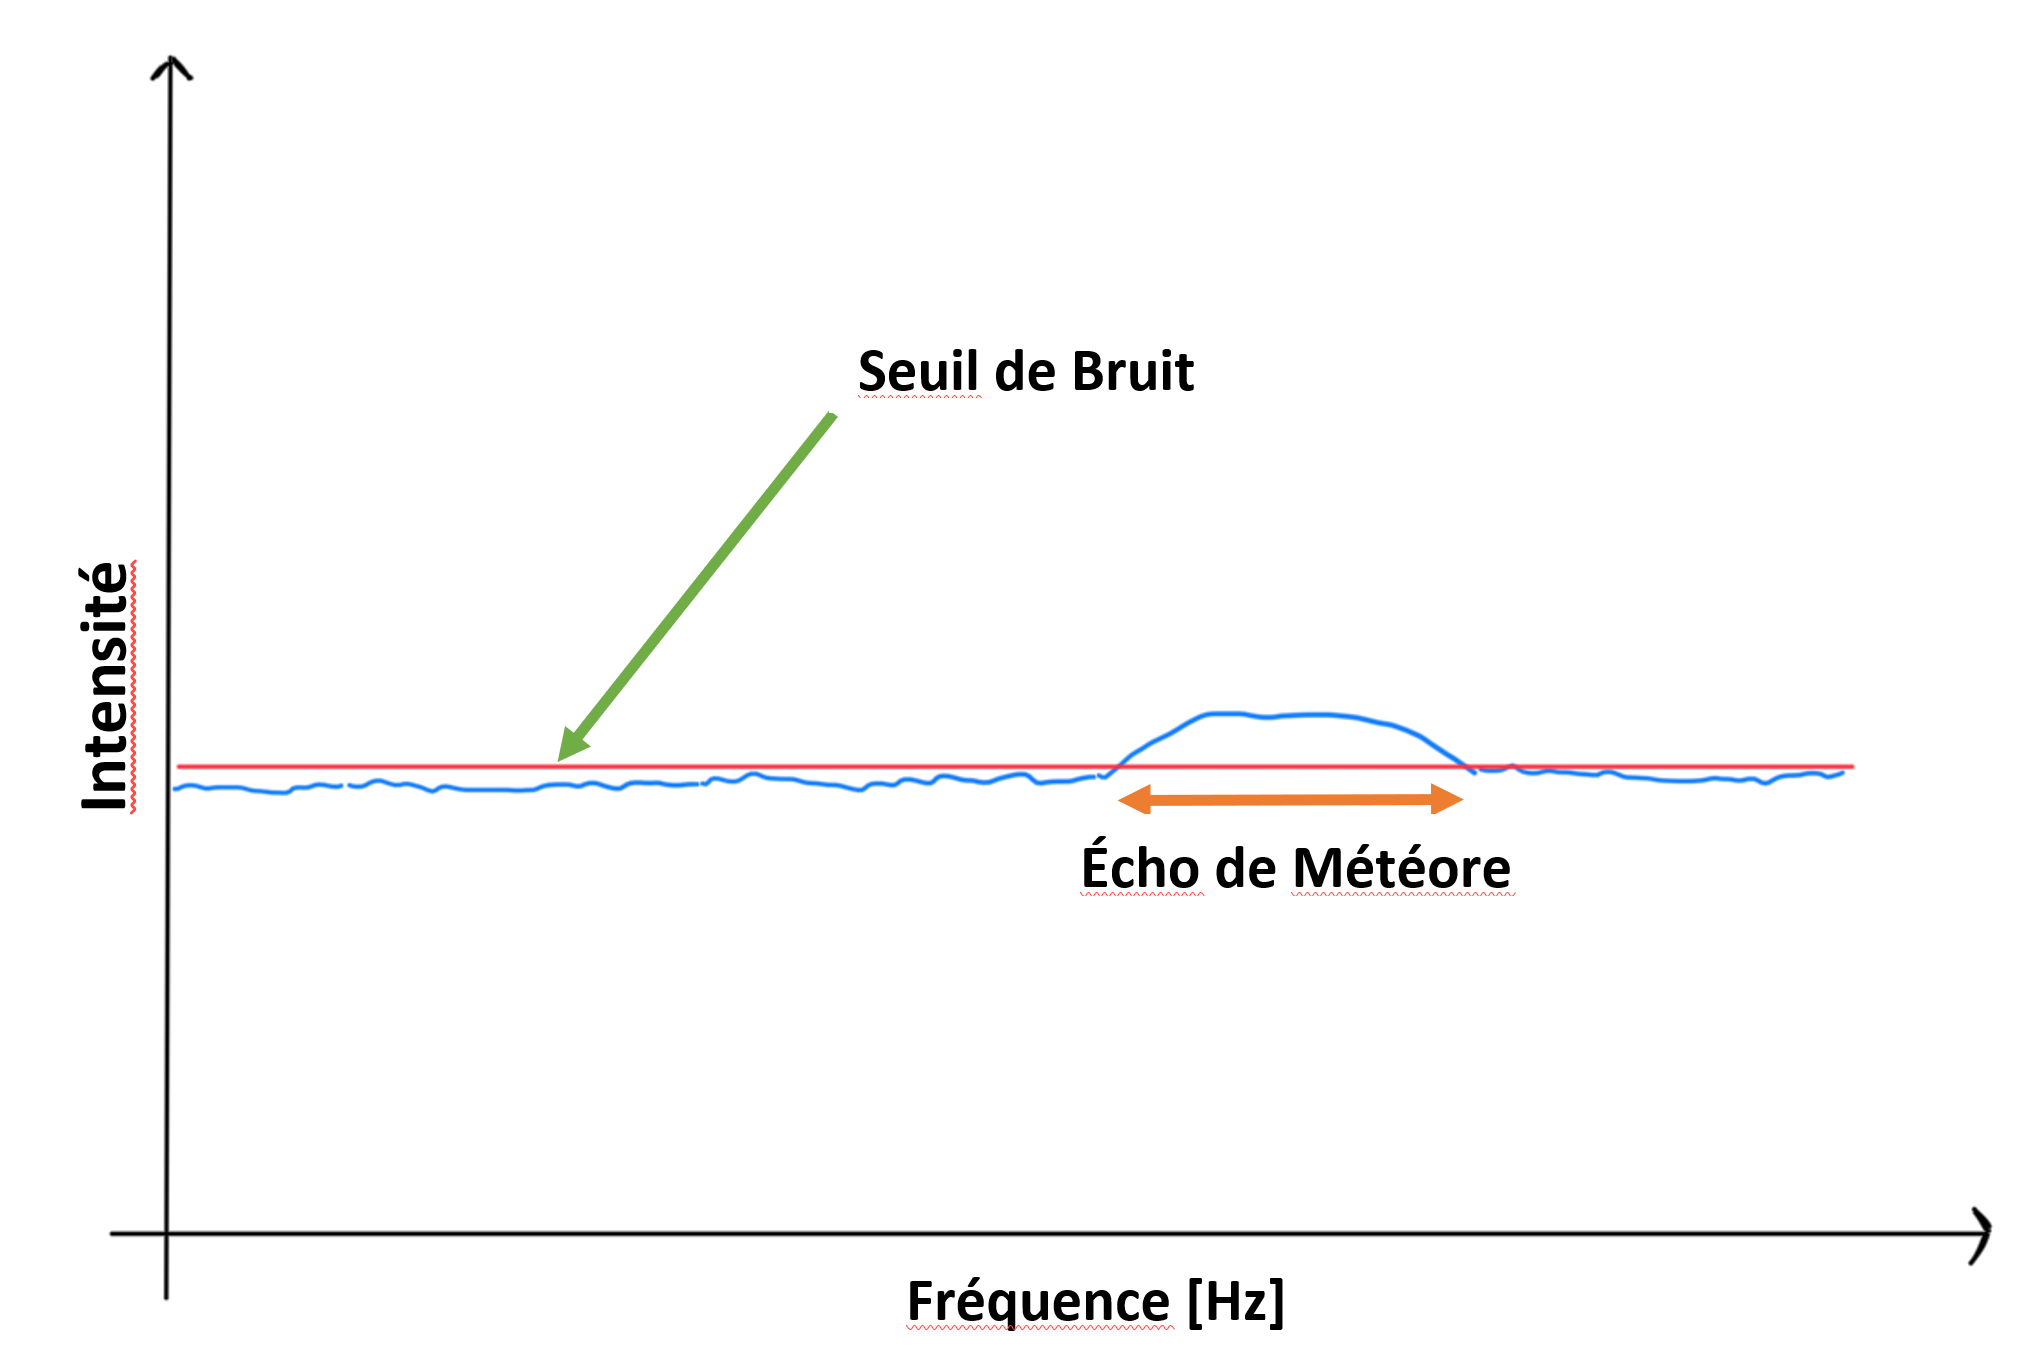
\includegraphics[scale=0.4]{Screenshot 2022-08-14 235407.png}
        \caption{FFT contenant un écho de météore.}
        \label{fig:meteor-fft}
    \end{center}
\end{figure}

Il ne reste plus qu'à rechercher la fréquence minimale et la fréquence maximale sur lequel s'étend l'écho.
Ceci est fait en calculant la transformée de Fourier de l'intervalle pendant laquelle l'écho de météore dure.
Une fois qu'on a la FFT, le logiciel détermine un seuil de bruit à la 85e percentile.
Comme on peut le voir à la figure \ref{fig:meteor-fft}, ceci met en évidence l'écho de météore et permet de retrouver facilement sa fréquence minimale et maximale.\\

\begin{figure}[h]
    \begin{center}
        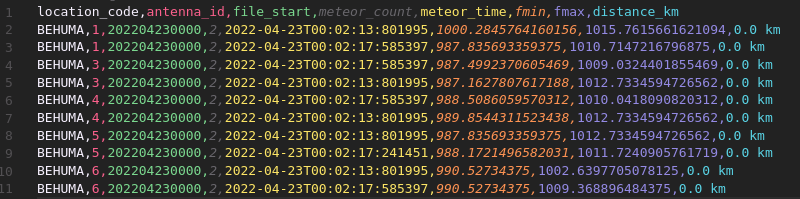
\includegraphics[scale=0.44]{Screenshot from 2022-05-31 16-35-06.png}
        \caption{Exemple de fichier CSV généré par le programme de détection de météores.}
        \label{fig:csv-example}
    \end{center}
\end{figure}

Enfin, le programme crée un fichier CSV qui contiendra une ligne par écho de météore détecté.
Chaque ligne contiendra :
\begin{enumerate}
    \item Le code de location de la station où est détecté l'écho.
    \item Le numéro de l'antenne qui a détecté l'écho.
    \item La date et le temps de début d'enregistrement du fichier d'où vient l'écho.
    \item Le nombres d'écho comptés dans le même fichier que celui d'où vient l'écho.
    \item Le temps, précis à la microseconde, de détection de l'écho.
    \item La fréquence minimum de l'écho.
    \item La fréquence maximum de l'écho.
    \item La distance entre la station où est détecté l'écho et la station reçue en entrée au lancement du programme.
\end{enumerate}

Un exemple de fichier CSV généré par le programme peut être visualisé à la figure \ref{fig:csv-example}.

\newpage

\section{Conclusion}

Le but principal de ce projet de fin d'études était de faciliter et automatiser une partie du travail des scientifiques du projet BRAMS.
Premièrement il devait permettre aux scientifiques de détecter rapidement une anomalie dans les données produites par les stations réceptrices.
Si un défaut n'est pas détecté rapidement, la station défectueuse continue à produire des données inutilisables.
Ce problème a été résolu grâce au logiciel de monitoring qui permet non-seulement de détecter une anomalie dans les données, mais également de visualiser la qualité des données grâce à son interface intégrée au site web BRAMS.
En effet, même si le logiciel alerte parfois l'utilisateur d'un problème non-existant et que des améliorations sont encore possibles, ces cas sont rares et le programme reste utilisable.\\
\\
Deuxièmement, le travail devait faciliter la recherche de tous les échos de météores pouvant correspondre à un météore spécifique.
Le programme de détection de météores permet aux scientifiques de grandement réduire le temps nécessaire pour chercher ces échos en retrouvant automatiquement tous les échos dans l'intervalle de temps nécessaire.\\
\\
Ce travail m'a également permis d'étendre mes connaissances dans le domaine du traitement du signal en mettant en pratique plusieurs notions théoriques vues durant les cours.
Le mélange de ces connaissances avec des nouvelles notions, que je n'avais pas encore appris, afin d'arriver à un résultat final a été un vrai défi pour moi.\\
\\
Enfin, ce projet m'a permis de contribuer à un projet scientifique de grande ampleur et m'a appris comment un tel projet fonctionne.

\newpage

\section{Perspectives}

Suite à une réflexion sur les programmes réalisés, j'ai listé ci-dessous quelques pistes d'améliorations intéressantes pour le futur :
\begin{itemize}
    \item Bien que cela ait déjà été dit, le remplacement du système de détection de météores, dans le programme qui retrouve les échos d'un météore, par le système plus avancé en développement par le projet BRAMS représenterait une réelle amélioration.
    \item Pour le programme qui retrouve les échos d'un météore, on pourrait, à terme, ajouter le facteur d'emplacement de la station pour retrouver les échos appartenant à un météore.
          Cependant, cela demande beaucoup de recherche et d'étude et prendrait donc un temps considérable.
    \item On pourrait ajouter la possibilité de manipuler l'entièreté du programme de monitoring à partir de son interface en ligne, sur le site de BRAMS.
    \item Actuellement, le programme de monitoring surveille les fichiers de façon à détecter des erreurs connues.
          Cependant, il est possible que des problèmes non connus surviennent, qui ne sont alors pas détectés par le logiciel de surveillance.
          Une amélioration intéressante serait donc de réfléchir à des potentiels erreurs qui ne seraient pas détectés et en tenir compte dans le programme.
    \item Il serait intéressant d'avoir une interface graphique sur le site web de BRAMS permettant de manipuler le programme qui recherche les échos venant d'un météore.
          Cette interface pourrait alors afficher ces résultats sur un spectrogramme en plus de générer un fichier CSV.
    \item Pour le système de détection d'anomalies dans le programme de monitoring, il serait intéressant d'effectuer plus de tests et de recherches afin d'améliorer la méthode utilisée.
          En effet, comme expliqué avant, il n'est pas parfait et alerte parfois l'utilisateur d'un problème alors qu'il n'y en a pas.
\end{itemize}

%? OLD

% \section{Lecture des Fichiers BRAMS}

% Avant de commencer à développer des outils pour la détection des météores ou pour l'analyse des fichiers BRAMS, il a fallu développer un logiciel permettant de lire ces fichiers.
% Ce logiciel sera implémenté dans un module Python contenant une classe nommée BramsWavFile.²
% Ceci veut dire qu'il pourra facilement être utilisé par d'autres fichiers Python et qu'il doit donc être flexible.
% Dans cette section, le fonctionnement de ce module est expliqué en détail.

% \subsection{Fonctionnement du Module}

% Le contenu principal du module est donc la classe BramsWavFile.
% Cette classe permet de lire et de récupérer des informations sur les fichiers WAV du réseau BRAMS de manière efficace.
% Elle est basée sur un code écrit par Michel Anciaux, membre du projet BRAMS.
% Cependant, elle a fortement été retravaillé afin de l'adapter aux besoins du programme et de l'optimiser.
% La classe prend six paramètres en entrée :

% \begin{itemize}
%     \item Le paramètre \textbf{date\_time} indique le temps et la date du fichier recherché.
%           Ce paramètre est obligatoire et doit être de type datetime, type qui est défini dans le module datetime.
%     \item Le paramètre \textbf{station} indique le code de location de la station recherchée (e.g. BEHUMA, BEHAAC, BEUCCL).
%           Les deux premières lettres de ce code représentent le code pays (e.g. BE, FR).
%           Typiquement, les quatre lettres suivantes sont les quatre premières lettres de la ville ou se trouve la station.
%           Ce paramètre est obligatoire et doit être de type str (chaine de caractères).
%     \item Le paramètre \textbf{alias} indique l'antenne, se trouvant à la location spécifiée, dont on veut récupérer un fichier.
%           En effet, certaines stations disposent de plusieurs antennes.
%           Les antennes sont spécifiées à l'aide de six caractères : les trois premiers contiennent les lettres 'SYS' et les trois suivants contiennent le numéro de l'antenne (e.g. 001, 002, ...).
%           La valeur par défaut de ce paramètre est 'SYS001', c'est donc un paramètre optionnel.
%           Le type du paramètre est str (chaine de caractères).
%     \item Le paramètre \textbf{is\_wav} est un booléen indiquant à la classe si le fichier recherché se trouve dans un fichier de format TAR (dans quel cas la valeur devrait être 'faux') ou pas (dans quel cas la valeur devrait être 'vrai').
%           Ce paramètre est optionnel et prend la valeur 'faux' par défaut.
%     \item Le paramètre \textbf{parent\_directory} indique le répertoire parent ou il faudra commencer la recherche du fichier demandé.
%           C'est un paramètre optionnel de type str (chaine de caractère) qui prend le répertoire de l'archive BRAMS comme valeur par défaut.
%     \item Le paramètre \textbf{from\_archive} est un booléen indiquant si le fichier recherché se trouve dans un répertoire respectant la structure de l'archive BRAMS (dans quel cas la valeur est 'vrai') ou non (dans quel cas la valeur est 'faux').
%           Elle prend la valeur 'vrai' par défaut et est donc optionnel.
% \end{itemize}

% Lorsque la classe est initialisée, elle vérifie d'abord si le fichier recherché existe.
% Si le paramètre 'from\_archive' contient la valeur 'vrai', la classe rajoute, au chemin spécifié par le paramètre 'parent\_directory', les dossiers nécessaires pour que le chemin respecte la structure de l'archive BRAMS.
% Ensuite, le programme essaye de lister les contenus du dossier.
% Dans le cas ou le dossier n'est pas trouvé, l'initialisation de la classe est interrompue et l'exception 'DirectoryNotFoundError' est levée.\\
% \\
% La classe recherche ensuite pour le bon fichier dans le contenu du répertoire en comparant la date et le temps dans le nom du fichier avec la date et le temps reçu comme paramètre.
% Quand les fichiers WAV sont contenus dans une archive TAR, l'étape précédente est répétée pour trouver le bon fichier dans l'archive.
% Si aucun fichier correspondant à la date et la station reçue en paramètres est trouvé, l'initialisation de la classe est interrompue et l'exception 'BramsError' est levée.
% Une fois le bon fichier trouvé, toutes les données brutes sont lues et enregistrées dans un buffer (variable).\\
% \\
% La prochaine étape est la séparation des différents blocs de données (ou chunk) contenus dans le fichier WAV.
% Pour ça, la classe parcourt le buffer contenant les données du fichier WAV.
% Il utilise un pointeur de lecture indiquant la position en octets du prochain bloc de données dans le buffer.
% Ce pointeur est calculé à partir du champ 'subChunkSize' indiquant la longueur du bloc de données courant.\\
% \\
% Lorsque le programme retrouve un bloc de données avec un champ ID correspondant à 'fmt ', 'BRA1' ou 'data', il extrait toutes ces données et les place dans un ndarray.
% Ceci est fait à l'aide de la fonction 'frombuffer' venant de la librairie NumPy.
% Cette fonction offre la possibilité de convertir, de façon très rapide, des données vers un ndarray.
% Une des contraintes pour utiliser cette fonction est l'indication du type de données qu'on veut placer dans un ndarray.\\
% \\
% Les données contenues dans la classe seront la fréquence d'échantillonnage, extrait du bloc de données 'BRA1', et la piste audio du fichier WAV, extrait du bloc de données 'data'.

% \subsubsection{La méthode FFT}

% La classe BramsWavFile dispose d'une méthode publique.
% Cette méthode se nomme 'FFT' et permet, comme son nom l'indique, de récupérer la Transformée de Fourier de l'entièreté de la piste audio du fichier WAV.
% Ceci est fait à l'aide de la fonction 'rfft' de la librairie Scipy, multipliée par une fenêtre de Hann.
% La fonction 'rfft' existe également dans la librairie NumPy, cependant dans ce cas de figure la librairie SciPy permettait de calculer la Transformée de Fourier plus rapidement.
% Enfin, la fonction FFT retourne la Transformée de Fourier normalisée, son abscisse et sa résolution fréquentielle.\\
% \\
% Le code de cette méthode peut être visualisé à la figure 8.

% \begin{figure}
%     \begin{lstlisting}[style=CStyle]
% def FFT(self, Isamples, force_new=False):
%     if (
%         self.fft is not None
%         and self.fft_fbin is not None
%         and self.fft_freq is not None
%         and not force_new
%     ):
%         return self.fft_freq, self.fft, self.fft_fbin

%     # get the length of all the audio samples
%     nsamples = Isamples.size

%     # create a window funtion
%     w = windows.hann(nsamples)
%     w_scale = 1 / w.mean()

%     # apply that window on all the audio samples
%     Isamples = Isamples * w * w_scale

%     # get the Fourier Tranform and normalize it
%     S = rfft(Isamples) / nsamples
%     S[1: -1] *= 2

%     self.fft = S
%     self.fft_fbin = self.fs / nsamples
%     self.fft_freq = rfftfreq(nsamples, 1 / self.fs)

%     return self.fft_freq, S, self.fft_fbin
%     \end{lstlisting}
%     \caption{Code de la méthode qui génère une Transformée de Fourier sur base de données audio.}
% \end{figure}

% \newpage

% \section{Monitoring des Données BRAMS}

% Comme indiqué précédemment, les fichiers ne contiennent pas toujours des données utilisables.
% Pour des diverses raisons, il peut parfois arriver que le bruit est trop fort pour pouvoir détecter des météores.
% Ou encore, lorsque les stations ICOM arrivent en fin de vie, la puissance des données détectées décroît de telle sorte qu'on détecte du bruit seulement.
% Bref, de nombreux problèmes peuvent survenir avec les données.
% Pour optimiser la détection de météores, les données corrompus doivent être détectés avant celle-ci.
% C'est pourquoi, un outil permettant le monitoring des données a été développé.\\
% \\
% Cet outil se base sur deux éléments dans les données BRAMS indiquant si un fichier est utile ou non.
% Le premier est le bruit.
% En effet, lorsque le bruit augmente ou diminue beaucoup d'un coup ou graduellement sans revenir à un niveau normal, il est fort probable qu'il y ait un problème avec la station réceptrice ou son environnement.\\
% \\
% Le deuxième élément permettant de détecter un problème est le signal du calibreur.
% Le signal calibreur devrait toujours être présent dans un fichier produit par une station réceptrice.
% Typiquement elle devrait se trouver autour de la fréquence 1500 Hz.
% Cependant, avec les anciennes stations, elle peut varier jusqu'à 250 Hz dépendant de la chaleur.
% Dans le cas où elle n'est pas aux alentours de 1500 Hz, la probabilité qu'il y ait une erreur avec la station est grande.

% \subsection{Fonctionnement du Programme}

% \begin{figure}
%     \begin{lstlisting}[style=CStyle]
% def get_psd(f, flow=800, fhigh=900):
%     # get fourier tranform from BramsWavFile class
%     freq, S, fbin = f.FFT(f.Isamples)
%     idx = (freq >= flow) * (freq < fhigh)

%     # calculate the total power of the wanted frequencies
%     p = (S[idx] * S[idx].conj()).real / 2

%     # get a mean normalized to 1Hz
%     psd = p.mean() / fbin

%     return psd
%     \end{lstlisting}
%     \caption{Code de la fonction permettant de calculer la dsp.}
% \end{figure}

% Le programme permet donc de mesurer le niveau du bruit et le signal calibreur d'un ou de plusieurs fichiers WAV du projet BRAMS.
% Il fait ceci en calculant la densité spectrale de puissance (dsp) de ceux-ci.
% La densité spectrale de puissance montre la distribution des puissances à travers les différentes fréquences contenues dans le signal de base.
% Ceci permet de comparer ces différentes valeurs et de remarquer des variations non typiques.\\
% \\
% Lorsqu'on lance le programme, trois paramètres peuvent être ajoutés :
% \begin{enumerate}
%     \item Le paramètre \textbf{START DATE} indique la date à partir de laquelle on veut mesurer la dsp des fichiers.
%           Par défaut, elle prendra la date d'un jour avant le lancement du programme.
%     \item Le paramètre \textbf{END DATE} indique la date avant laquelle on veut mesurer la dsp des fichiers.
%           Dans le cas où le paramètre 'START DATE' n'est pas donné, elle prend la valeur de la date de lancement du programme.
%     \item Le paramètre \textbf{STATIONS} indique les stations pour lesquelles on veut mesurer la dsp des fichiers.
%           Si ce paramètre n'est pas donné, le programme mesurera la dsp des fichiers de toutes les stations.
% \end{enumerate}

% Le programme calculera donc la dsp des fichiers de tous les fichiers générés entre \textbf{START DATE} et \textbf{END DATE} venant des stations \textbf{STATIONS}.\\
% \\
% La première va donc, pour chaque fichier demandé, performer une suite d'étapes.
% Premièrement, elle va chercher le fichier à l'aide de la classe 'BramsWavFile'.
% Si une erreur se produit lors de la recherche du fichier, on considère que le fichier n'existe pas et le programme passe au fichier suivant.
% Lorsqu'on a le fichier, on peut calculer la dsp du bruit et du signal calibreur.
% La fonction permettant de calculer la dsp, peut être visualisée à la figure 9.\\
% \\
% Dans le cas du bruit, on prend toujours la moyenne de la dsp entre 800 Hz et 900 Hz.
% Entre ces deux fréquences on retrouve normalement uniquement du bruit.
% Dans les cas où il se trouverait qu'il y ait un signal autre que le bruit, il ne devrait pas avoir grand impact sur la dsp puisque cette dernière se calcule sur 100 Hz, sur l'entièreté d'un fichier.\\
% \\
% Pour le signal calibreur, in ne suffit pas de calculer la moyenne de la dsp à 1500 Hz.
% En effet, la fréquence du calibreur peut varier jusqu'à 250 Hz, autour de la fréquence de 1500 Hz, d'un fichier à l'autre.
% Comme le signal calibreur est le seul signal se trouvant entre 1350 Hz et 1750 Hz, il suffit de rechercher la fréquence, entre ces deux valeurs, avec la valeur de dsp maximale.\\
% % \\
% % Lorsque les deux valeurs de dsp ont été calculées, on peut maintenant détecter d'éventuels variations atypiques par rapport à d'anciennes valeurs.
% % Premièrement, le programme ajuste une droite sur les valeurs de dsp du bruit allant de la date du fichier actuel jusqu'à 
% \\
% Enfin, le programme enregistre toutes les données de dsp dans la base de données BRAMS existante.
% Chaque valeur de dsp est alors lié à son fichier.
% Si l'option \textbf{-p} (\textbf{--plot}) a été donné au lancement du programme, le programme génère également un graphique représentant l'évolution de la dsp au cours du temps.

% \subsection{Résultats}

% \begin{figure}[t]
%     \begin{center}
%         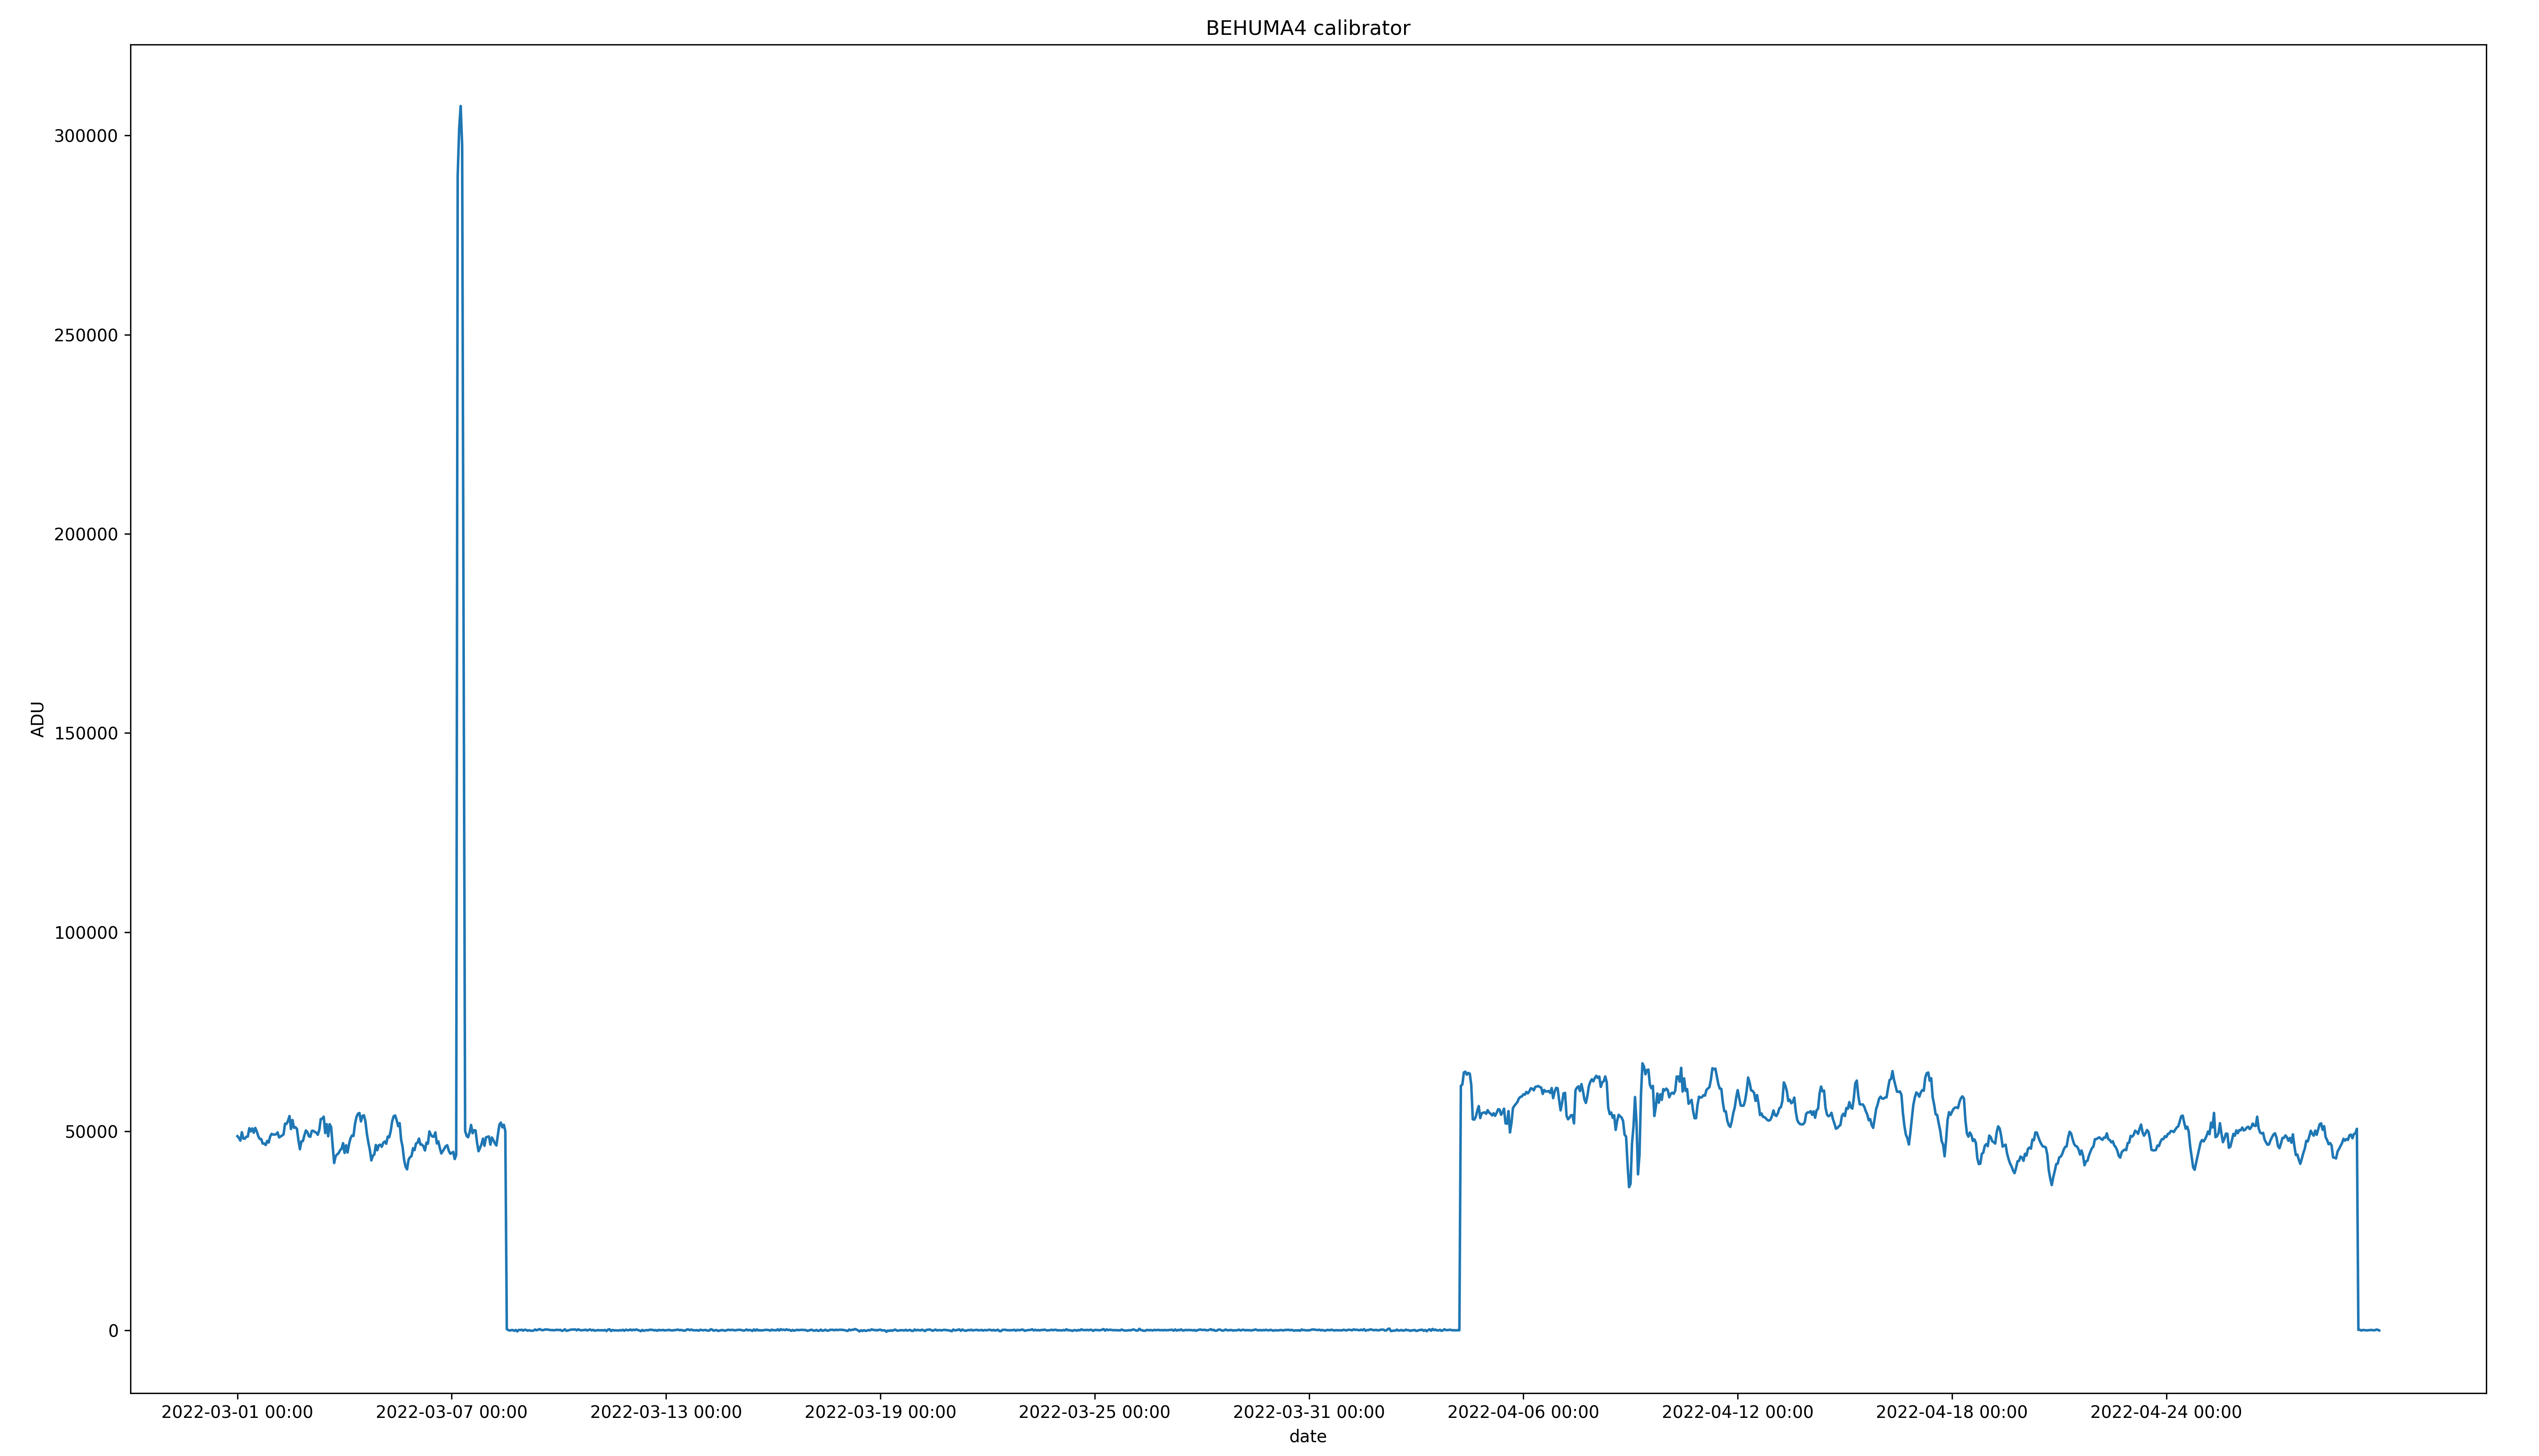
\includegraphics[scale=0.235]{BEHUMA4_2022-03-01_2022-04-30_calibrator.png}
%         \caption{Signal calibreur de la station BEHUMA, antenne 4 entre le 1\textsuperscript{er} mars 2022 et le 30 avril 2022.}
%     \end{center}
% \end{figure}

% Lors des tests, quelques résultats ont déjà montrés des informations intéressantes.
% Un bon exemple est l'antenne quatre de la station à Humain entre le 1\textsuperscript{er} mars 2022 et le 30 avril 2022, à la figure 10.
% On remarque qu'à partir 8 mars 2022, le signal calibreur diminue fortement d'intensité.
% Après une étude en profondeur par les scientifiques du projet BRAMS, ils ont trouvé que ceci était dû à un problème avec l'oscillateur local.
% Ce problème causait une translation de 500 Hz vers le bas de tout signal.
% Ceci veut dire que tous les fichiers générés alors qu'il y avait ce problème sont inutilisables.\\
% \\
% Un autre exemple est la station à Haacht entre le 1\textsuperscript{er} juillet 2021 et le 31 août 2021 affichée à la figure 11.
% Ici, on constate une diminution graduelle de l'intensité du bruit, jusqu'�� ce que le récepteur ne capte plus rien.
% Ceci est causé suite au vieillissement du récepteur ICOM.
% Cette station a donc dû être remplacée.

% \begin{figure}[t]
%     \begin{center}
%         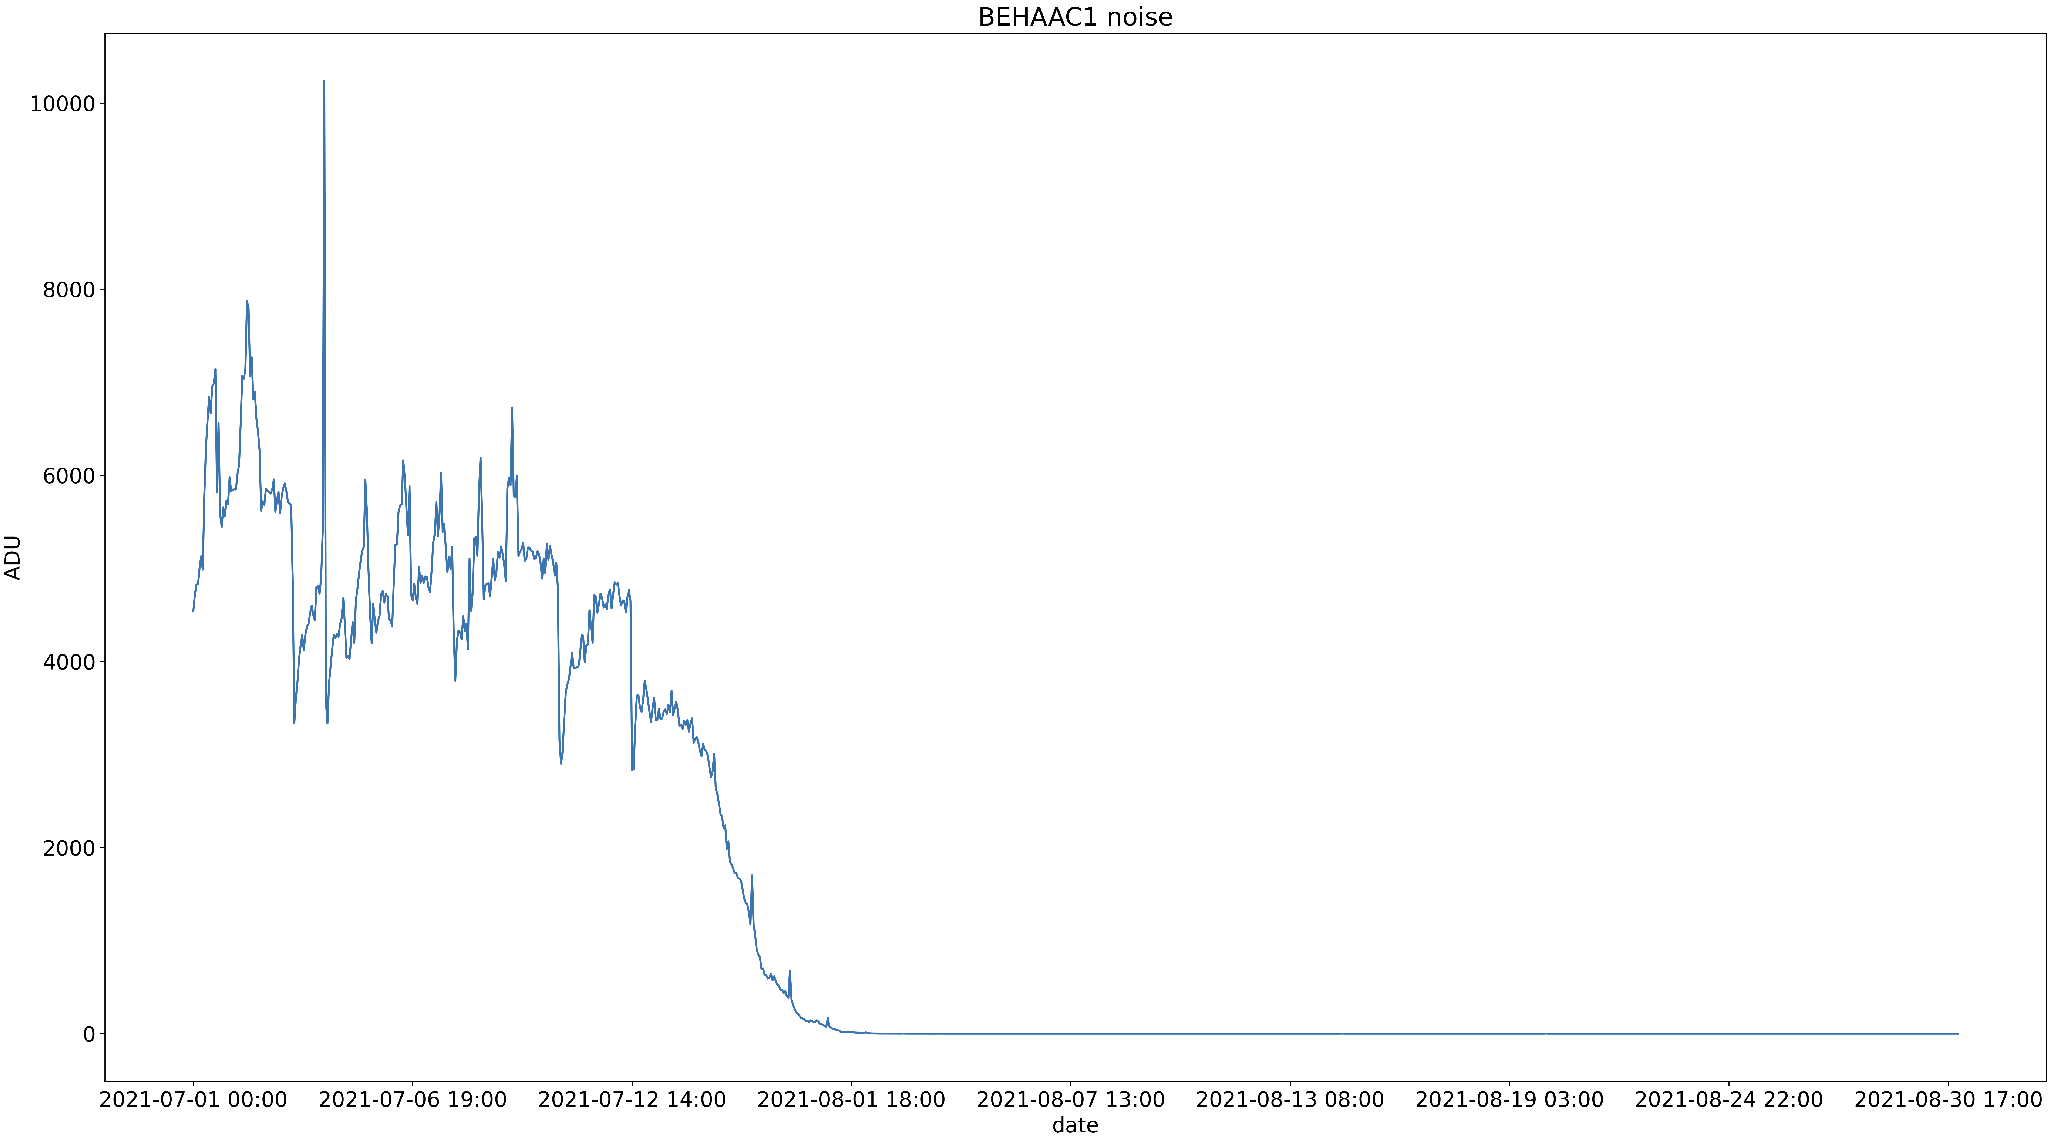
\includegraphics[scale=0.235]{BEHAAC1_2021-07-01_2021-08-31_noise.png}
%         \caption{Intensité du bruit de la station BEHAAC, antenne 1 entre le 1\textsuperscript{er} juillet 2021 et le 31 août 2021.}
%     \end{center}
% \end{figure}

% \newpage

% \section{Détection des Météores}

% Finalement, on arrive à la détection des météores.
% Ce programme effectue deux tâches principales.
% La première tâche consiste à, à partir des coordonnées d'un météore donné, détecté sur une station donnée, trouver tous les échos qui viennent potentiellement du même météore.
% Ensuite, la deuxième tâche du programme est de donner l'utilisateur le plus d'informations possibles pour confirmer qu'un écho correspond à l'écho de météore reçu en entrée ou non.

% \subsection{Analyse}

% \begin{figure}[t]
%     \begin{center}
%         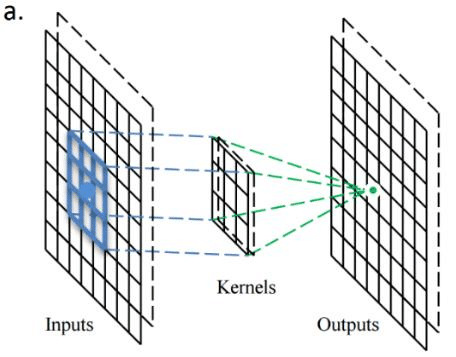
\includegraphics[scale=0.6]{a-Illustration-of-the-operation-principle-of-the-convolution-kernel-convolutional-layer.png}
%         \caption{Illustration de la convolution.}
%     \end{center}
% \end{figure}

% C'est ici la première étape qui pose la plus grande difficulté.
% En effet, la détection de météores consiste à retrouver des objets d'une forme spécifique dans une image.
% Cette image est, dans ce cas si, un spectrogramme calculé à partir d'un fichier WAV venant d'une station de réception BRAMS.
% De plus, on retrouve sur ce spectrogramme un nombre d'autres parasites que le programme doit pouvoir différencier d'un vrai météore tel que les échos d'avions qui passent, ou encore le signal direct de l'émetteur.\\
% \\
% Afin de faciliter la rechercher d'échos de météores dans un spectrogramme, l'amplification de ces échos peut faciliter la tâche.
% Un écho de météore est, dans un spectrogramme, caractérisé par un signal qui s'étale sur minimum 10 Hz et qui dur typiquement entre une et trois secondes.
% Ceci est possible en performant une convolution sur le spectrogramme.
% Une convolution est une opération mathématique qui prend deux fonctions en entrée et qui produit un nouveau signal.
% Dans ce cas si, le  signal en entrée sera le spectrogramme, ou une partie du spectrogramme, et le deuxième signal est le filtre.
% Une illustration de la convolution peut être trouvée à la figure 12.
% Afin d'arriver à un bon résultat, il a fallu tester plusieurs filtres.
% Le filtre offrant les meilleurs résultats est illustré à la figure 13.
% Elle permet de faire deux choses :

% \begin{itemize}
%     \item Premièrement, elle amplifie les éléments qui font plus de 10 Hz.
%           En effet, pour avoir un résultat d'une valeur maximale il faut que le haut et le bas du filtre soient multipliées par des grandes valeurs.
%     \item Deuxièmement, elle permet de diminuer l'intensité des éléments qui ont une longue forme horizontale (typiquement des échos d'avions).
% \end{itemize}

% Suit alors la suppression du signal direct de l'émetteur.
% En effet, pour détecter les échos de météores, le signal direct nous complique la tâche.
% Pour l'éliminer, le programme recherche d'abord sa fréquence entre 800 Hz et 1200 Hz, en prenant la valeur maximale sur l'entièreté de la durée du fichier, entre ces deux fréquences.
% S'il n'est pas retrouvé, on considère qu'il n'est pas détecté (ce qui est le cas sur certaines stations réceptrices).
% Par contre, dans le cas où il est détecté, pour chaque seconde, on remplace la valeur du signal direct par la moyenne des valeurs se trouvant autour de la fréquence du signal direct.\\
% \\
% Ensuite, il faut trouver une méthode permettant de séparer, dans le spectrogramme, les objets du bruit.
% La première méthode testée se basait sur un seuil fixe.
% Toutes les valeurs qui se trouvaient en dessous de ce seuil étaient considérées comme du bruit et leur valeur était mise à zéro.
% Bien que cette méthode fonctionnait bien sur un fichier spécifique, elle posait problème si on voulait la lancer sur plusieurs fichiers différents.
% En effet, comme toutes les stations de réception se trouvent dans des environnements différents et disposent parfois même de matériel différent, différent fichier ont des niveaux de bruits différents.\\
% Pour la deuxième méthode, le programme essayait de trouver un seuil qui se base sur la valeur du bruit sur l'entièreté d'un spectrogramme.
% Pour ce faire, la méthode divisait le spectrogramme, entre les fréquences de 600 Hz et 1400 Hz, en trente zones.
% Elle mesurait ensuite, à l'aide de la variance de chaque zone, laquelle contenait le moins d'objets possibles.
% Finalement, la méthode calculait la 95e percentile du bloc contenant le moins d'objet possibles.
% Toutes les valeurs du spectrogramme se trouvant en dessous de cette valeur seraient considérés comme du bruit et mises à zéro.
% Malgré que cette méthode produisait des résultats marginalement meilleurs que celle à seuil fixe, elle n'était toujours pas parfaite étant donné qu'elle se basait sur le bruit d'une partie du spectrogramme, or le bruit peut varier au cours du temps.\\
% Finalement, la méthode qui fonctionnait le mieux calculait la 95e percentile pour chaque colonne du spectrogramme.
% Ensuite, elle remplace toutes les valeurs de cette colonne se trouvant en dessous de la 95e percentile avec zéro.
% Les résidus de bruits qui ne sont pas encore éliminés sont négligeables puisqu'ils s'étalent sur moins de 10 Hz et ne sont donc pas considérés comme des météores.\\
% \\
% Il faut maintenant éliminer tous les objets qui ne sont pas des échos de météores, mais qui s'étalent sur plus de 10 Hz.
% Ceci n'est pas une tâche facile puisque des parasites peuvent venir se mélanger à des échos de météore formant un objet.
% La première chose à faire est : nettoyer le spectrogramme des petits parasites, ou encore de résidus de bruits.
% Le programme fait cela en labellisant le spectrogramme et en éliminant tout objet s'étalant sur moins de 10 Hz.
% Ensuite, on récupère tous les objets restants.
% Pour chacun de ces objets, on vérifie s'il n'est pas composé de plusieurs parasites se superposant sur plus de 10 Hz.
% Ceci est fait en allant vérifier sur une longueur d'environ treize secondes autour de l'objet détecté, si on retrouve des parasites qui s'étalent sur la même fréquence que cet objet.
% Lorsque c'est le cas, l'objet n'est pas considéré comme un météore et est ignoré.
% À partir de ce stade, tous les objets détectés sont considérés comme étant des échos de météores.\\
% \\
% Pour la deuxième étape, le programme récolte le plus d'informations possibles à propos des échos pouvant potentiellement correspondre à l'écho de météore reçu en entrée.
% Parmi ces informations, on retrouve tout d'abord le temps où un écho s'est produit.
% Ceci est important pour pouvoir situer l'écho si on veut l'étudier en profondeur.\\
% Ensuite, le programme calcule la distance entre la station qui a détecté l'écho reçu en entrée et la station dont un écho pourrait correspondre à celui en entrée.
% En effet, un météore n'est pas détecté par toutes les stations, et dans le cas où il est détecté par plusieurs stations, ces stations se trouvent souvent proches les uns des autres.\\
% La troisième information donnée indique le nombre d'échos trouvés pour une station, pouvant correspondre à l'écho en entrée.
% Dans ce cas, il est important d'en informer l'utilisateur, puisque ces échos viennent chacun d'un météore différent et ne peuvent donc pas tous venir de cet écho reçu en entrée.\\
% La dernière information donnée par le programme sont la fréquence minimum et la fréquence maximum des échos détectés.
% Ces deux fréquences permettront, ensemble avec le temps où l'écho s'est produit, de faciliter la recherche de cet écho pour l'utilisateur.

% \begin{figure}
%     \begin{lstlisting}[style=CStyle]
%         [[ 0.   0.   0.  50.   0.   0.   0. ]
%          [ 0.   0.   0.  50.   0.   0.   0. ]
%          [ 0.   0.   0.   0.   0.   0.   0. ]
%          [ 0.   0.   0.   0.   0.   0.   0. ]
%          [ 0.   0.   0.   0.   0.   0.   0. ]
%          [ 0.   0.   0.   0.   0.   0.   0. ]
%          [ 0.   0.   0.   0.   0.   0.   0. ]
%          [ 0.   0.   0.   0.   0.   0.   0. ]
%          [ 0.   0.   0.   0.   0.   0.   0. ]
%          [ 0.   0.   0.   0.   0.   0.   0. ]
%          [ 0.   0.   0.   0.   0.   0.   0. ]
%          [ 0.   0.   0.   0.   0.   0.   0. ]
%          [-1.5  0.   0.   0.   0.   0.  -1.5]
%          [-1.5  0.   0.   0.   0.   0.  -1.5]
%          [-1.5  0.   0.   0.   0.   0.  -1.5]
%          [ 0.   0.   0.   0.   0.   0.   0. ]
%          [ 0.   0.   0.   0.   0.   0.   0. ]
%          [ 0.   0.   0.   0.   0.   0.   0. ]
%          [ 0.   0.   0.   0.   0.   0.   0. ]
%          [ 0.   0.   0.   0.   0.   0.   0. ]
%          [ 0.   0.   0.   0.   0.   0.   0. ]
%          [ 0.   0.   0.   0.   0.   0.   0. ]
%          [ 0.   0.   0.   0.   0.   0.   0. ]
%          [ 0.   0.   0.   0.   0.   0.   0. ]
%          [ 0.   0.   0.   0.   0.   0.   0. ]
%          [ 0.   0.   0.  50.   0.   0.   0. ]
%          [ 0.   0.   0.  50.   0.   0.   0. ]]
%     \end{lstlisting}
%     \caption{Filtre utilisé pour amplifier les échos de météores.}
% \end{figure}

% \subsection{Fonctionnement du Programme}

% \begin{figure}[t]
%     \begin{center}
%         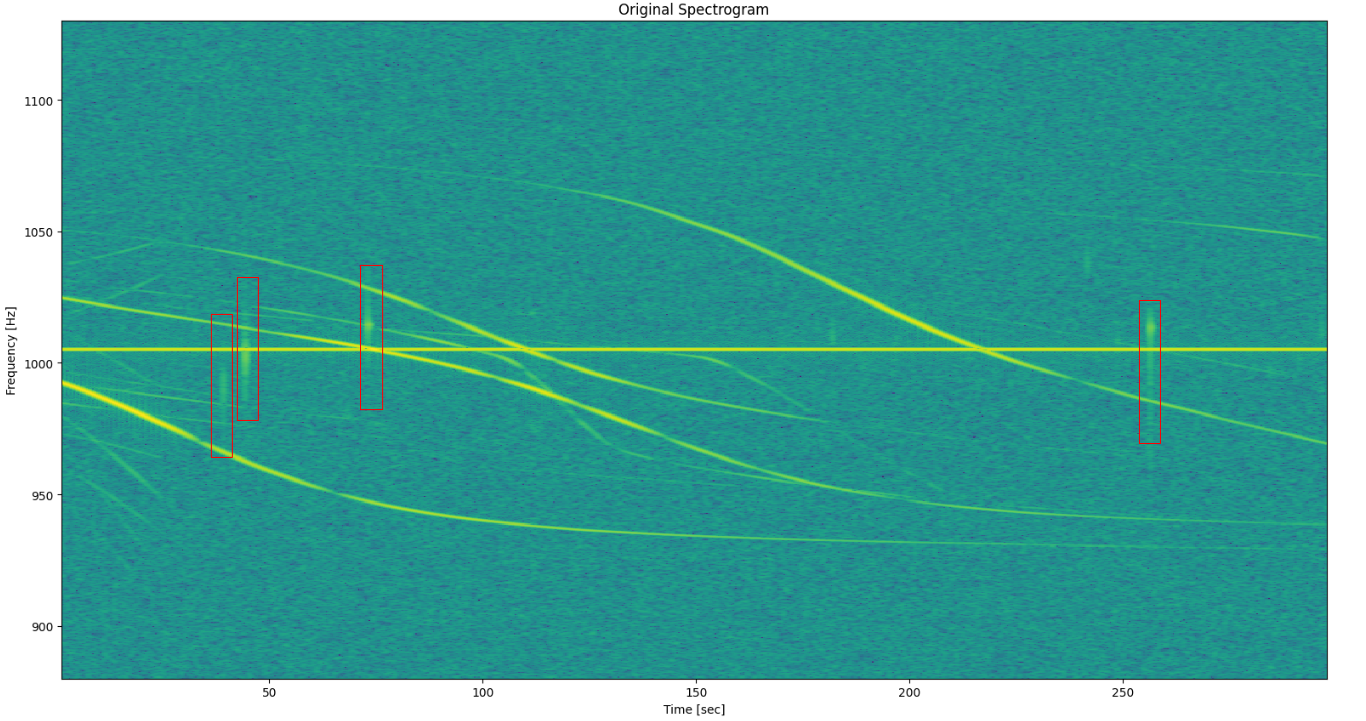
\includegraphics[scale=0.25]{Screenshot from 2022-05-31 16-44-50.png}
%         \caption{Spectrogram originale, sans modifications. Les échos de météores sont entourés en rouge.}
%     \end{center}
% \end{figure}

% Le programme prend en entrée le temps et la date de l'écho du météore recherché ainsi que le code de location de la station qui l'a détecté.
% À partir du temps et de la date reçue en entrée, le programme calcule l'intervalle de temps dans laquelle elle doit chercher des échos pour les autres stations réceptrices.
% Cet intervalle est toujours de six secondes autour du temps reçu en entrée.
% Cette valeur a été choisie puisque toute détection en dehors de ces six secondes a très peu de probabilité de venir du même météore que l'écho en entrée.
% Toutes les actions sur le spectrogramme s'appliqueront uniquement à l'intérieur de cet intervalle afin d'optimiser le programme.\\
% \\
% Le programme va ensuite chercher, pour toutes les stations, les informations des fichiers contenant cet intervalle.
% Il fait pour ça une requête à la base de données BRAMS.
% Puis, pour chaque station, le programme calcule la distance entre la station et la location où l'écho de météore reçu en entrée a été détecté.\\
% \\
% \begin{figure}[t]
%     \begin{center}
%         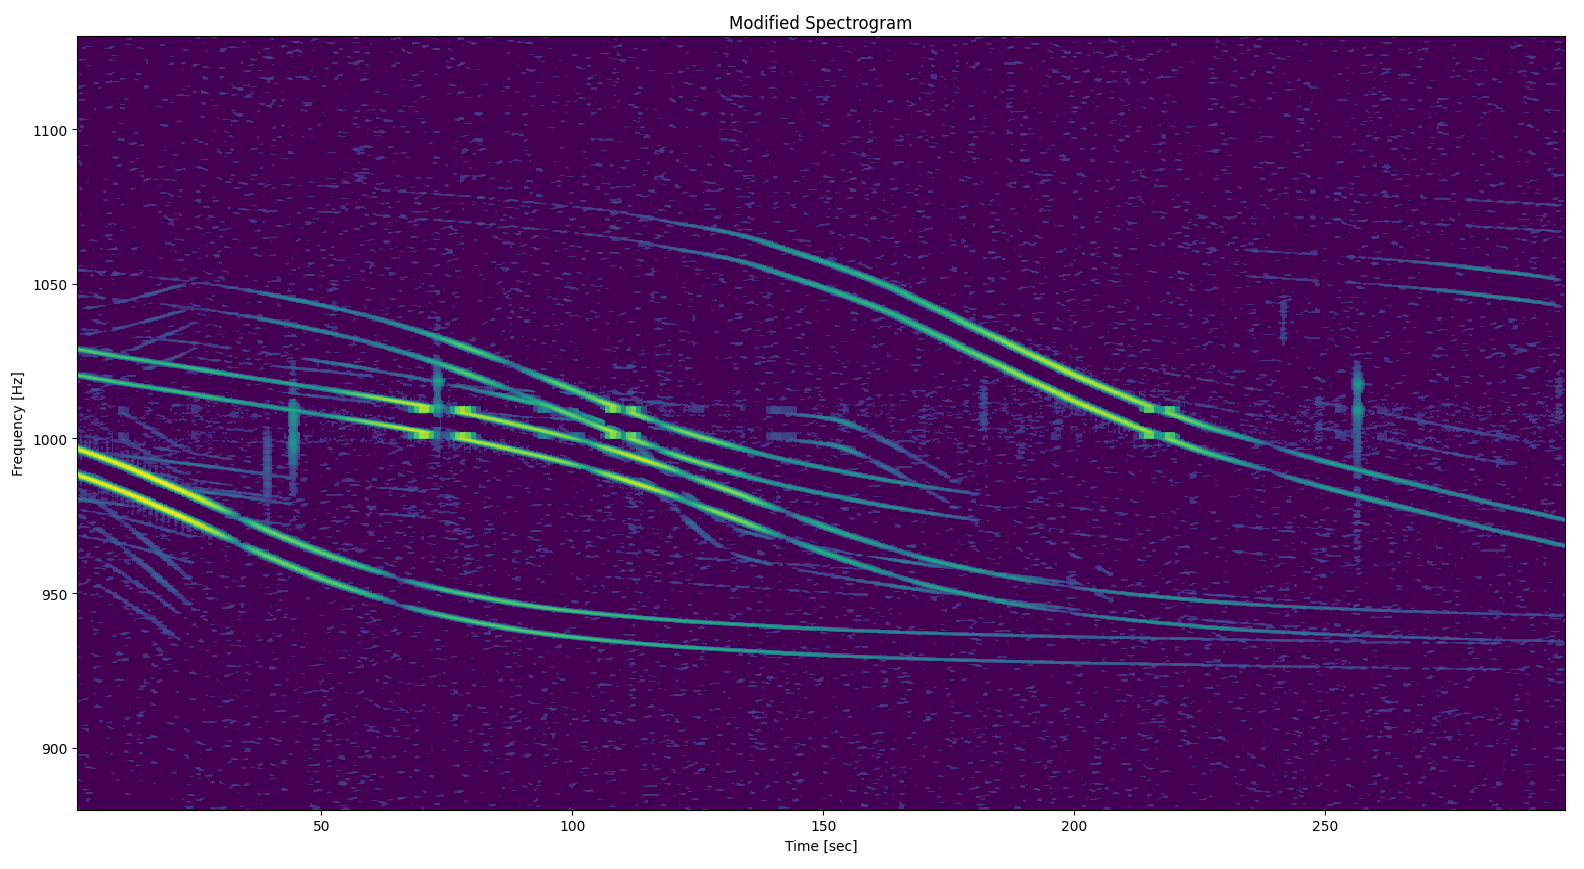
\includegraphics[scale=0.22]{Screenshot from 2022-05-31 16-32-43.png}
%         \caption{Spectrogramme après l'amplification des échos de météores et la suppression de la majorité du bruit.}
%     \end{center}
% \end{figure}
% Quatrièmement, pour tous les fichiers dont on a récolté des informations, on va rechercher les météores dans l'intervalle calculé précédemment.
% Pour cette étape, le programme fait d'abord appelle à la classe BramsWavFile, qui ira chercher le fichier et extraire les données audio.
% L'étape suivante consiste à générer le spectrogramme à partir de ces données audio.
% Afin de générer ce spectrogramme, il faut faire appelle à la classe Spectrogram.
% Ceci est une classe spécialement faite pour ce logiciel, qui permet de créer un spectrogramme et de le modifier à l'aide d'une suite de méthodes.
% Lorsqu'on appelle cette classe, il faut passer comme paramètre les données audio.
% À partir de ces données, la classe va créer le spectrogramme du fichier avec la fonction "scipy.signal.spectrogram()", un exemple du spectrogramme original peut être visualisé à la figure 14.
% La classe gardera une copie originale du spectrogramme et une copie pour les modifications, dont elle supprime, dès l'initialisation, le signal direct de l'émetteur.\\
% Suit alors une convolution du spectrogramme avec le filtre permettant d'amplifier les échos de météores, cette convolution est faite à l'aide de la fonction 'scipy.ndimage.convolve()'.
% Ensuite, le filtre supprimant toutes les valeurs en dessous de la 95e percentile sera appliquée.
% Un spectrogramme à ce stade est illustré à la figure 15, ce spectrogramme est le même que celui à la figure 14.
% Afin d'éliminer tous les résidus de bruits, le programme labellise le spectrogramme et supprime tout objet s'étalant sur plus de 6 Hz.
% Dans le but de reconnecter les météores qui auraient été divisés en deux parties différentes, on applique un filtre moyenneur sur le spectrogramme.
% Puis, le logiciel cherche les coordonnées des échos de météore sur le spectrogramme.
% Les météores trouvés sur le spectrogramme de la figure 14 et 15 sont affichées à la figure 16.
% En comparant les météores mise en évidence à la figure 14 et les échos trouvés par le programme à la figure 16, on constate que le programme arrive bien à retrouver les échos des météores.
% Avec ces coordonnées, on pourra alors retrouver la fréquence maximale et la fréquence minimale de l'écho.\\
% \\
% \begin{figure}[t]
%     \begin{center}
%         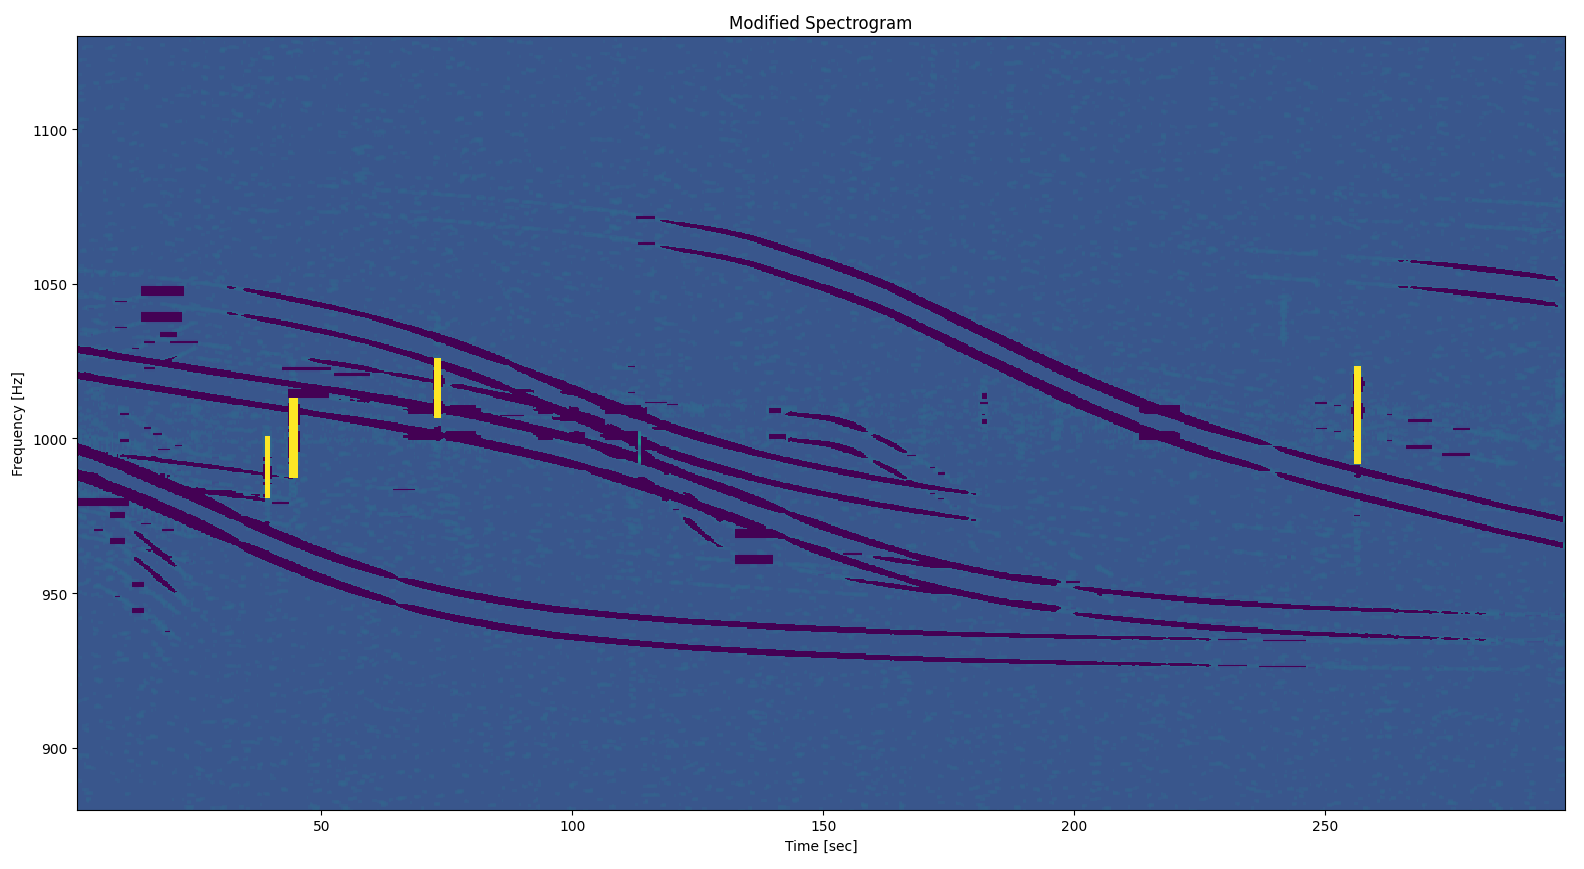
\includegraphics[scale=0.22]{Screenshot from 2022-05-31 16-33-53.png}
%         \caption{Spectrogramme après l'amplification des échos de météores et la suppression de la majorité du bruit.}
%     \end{center}
% \end{figure}
% Enfin, le programme crée un fichier CSV\footnote{Comma Separated Values} (figure 17) qui contiendra une ligne par écho de météore détecté.
% Chaque ligne contiendra :
% \begin{enumerate}
%     \item Le code de location de la station où est détecté l'écho.
%     \item Le numéro de l'antenne qui a détecté l'écho.
%     \item La date et le temps de début d'enregistrement du fichier d'où vient l'écho.
%     \item Le nombres d'écho comptés dans le même fichier que celui d'où vient l'écho.
%     \item Le temps, précis à la microseconde, de détection de l'écho.
%     \item La fréquence minimum de l'écho.
%     \item La fréquence maximum de l'écho.
%     \item La distance entre la station où est détecté l'écho et la station de l'écho reçu en entrée.
% \end{enumerate}

% De cette façon, les données pourront facilement être lues et réutilisées pour étudier ces météores.

% \begin{figure}[t]
%     \begin{center}
%         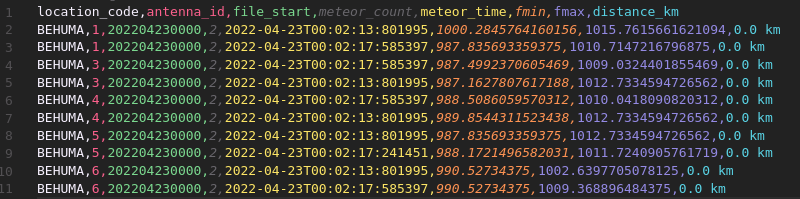
\includegraphics[scale=0.44]{Screenshot from 2022-05-31 16-35-06.png}
%         \caption{Exemple de fichier CSV généré par le programme de détection de météores.}
%     \end{center}
% \end{figure}

% \newpage

% \section{Pistes d'Améliorations}

% Suite à une réflexion sur les programmes réalisés, j'ai pu trouver quelques pistes d'améliorations qui sont intéressantes pour le futur :
% \begin{itemize}
%     \item Malgré que l'algorithme permettant de détecter des échos de météore fonctionne assez bien, il y a des cas où il détecte des échos là où il n'y en a pas et inversement.
%           En effet, lors de cas extrêmes (échos de météore faibles, superposition de nombreux parasites), le programme a parfois du mal à séparer les échos de météores du reste des objets.
%           Peaufiner cet algorithme permettrait d'éviter ces problèmes.
%     \item Lors de la détection des échos de météore, l'élimination du signal direct de l'émetteur est également un domaine qui peut être amélioré.
%           Actuellement, il est remplacé par la moyenne des valeurs situées autour de la fréquence du signal directe.
%           Cependant, ceci n'est pas l'idéal puisqu'on élimine une partie du signal utile avec cette méthode.
%           Une meilleure façon de l'éliminer est la reconstruction du signal directe, suivi de la soustraction.
%     \item Afin d'améliorer l'expérience utilisateur du programme, on pourrait ajouter ces deux programmes au site web BRAMS.
%           Ceci permet d'avoir un programme avec une interface plutôt que d'avoir un programme en ligne de commande.
%     \item Bien que ce n'est pas un point important, l'optimisation du programme permettrait d'avoir un temps d'exécution plus court.
%           Cela peut être achevé en essayant des librairies alternatives à NumPy et SciPy, ou encore à l'aide du développement de ses propres fonctions et méthodes.
% \end{itemize}

% \newpage

% \section{Conclusion}

% Le but du travail était d'automatiser deux procédures du projet BRAMS.
% Premièrement elle devait permettre aux scientifiques d'identifier les données corrompues et aider à retrouver la cause de ceux-ci.
% Ceci a été accompli à l'aide du logiciel de monitoring qui analyse les fichiers du projet BRAMS.\\
% \\
% Deuxièmement, le travail devait automatiser la recherche de tous les échos de météores pouvant correspondre à un météore spécifique.
% Cette tâche peut maintenant être complétée à l'aide du programme de détection de météore.\\
% \\
% Ce travail m'a permis d'étendre mes connaissances dans le domaine du traitement du signal en mettant en pratique plusieurs notions théoriques vues durant les cours.
% Le mélange de ces connaissances avec des nouvelles notions, que je n'avais pas encore appris, afin d'arriver à un résultat final a été un vrai défi pour moi.\\
% \\
% Enfin, ce projet m'a permis de contribuer à un projet scientifique de grande échelle.

\newpage

\begin{thebibliography}{100}
    \bibitem{brams_site}\textit{Site internet du projet BRAMS}, consulté en janvier 2022\\\url{https://brams.aeronomie.be/}
    \bibitem{sc.spectrogram}\textit{Documentation de la fonction scipy.signal.spectrogram}, consulté en février 2022\\\url{https://docs.scipy.org/doc/scipy/reference/ghttps://www.scribbr.com/statistics/outliers/enerated/scipy.signal.spectrogram.html}
    \bibitem{spectro1}\textit{Hands-On Tutorial on Visualizing Spectrograms in Python by Yugesh Verma}, consulté en février 2022\\\url{https://analyticsindiamag.com/hands-on-tutorial-on-visualizing-spectrograms-in-python/}
    \bibitem{spectro2}\textit{Cutting unused frequencies with specgram, matplotib by wwii}, consulté en février 2022\\\url{https://stackoverflow.com/questions/19468923/cutting-of-unused-frequencies-in-specgram-matplotlib}
    \bibitem{matplotlib}\textit{Documentation Matplotlib}, consulté en février 2022\\\url{https://matplotlib.org/stable/api/mlab_api.html#matplotlib.mlab.specgram}
    \bibitem{spectro3}\textit{Set spectrogram Parameters by rayryeng}, consulté en février 2022\\\url{https://stackoverflow.com/questions/29321696/what-is-a-spectrogram-and-how-do-i-set-its-parameters}
    \bibitem{convolve}\textit{Documentation de la fonction numpy.convolve}, consulté en mars 2022\\\url{https://numpy.org/doc/stable/reference/generated/numpy.convolve.html}
    \bibitem{convolve2}\textit{How to convolve two 2-dimensional matrices in python with scipy by Benjamin H.G. Marchant}, consulté en mars 2022\\\url{https://moonbooks.org/Articles/How-to-do-a-simple-2D-convolution-between-a-kernel-and-an-image-in-python-with-scipy-/}
    \bibitem{blocs}\textit{Slice 2D array in smaller 2D arrays by unutbu}, consulté en mars 2022\\\url{https://stackoverflow.com/questions/16856788/slice-2d-array-into-smaller-2d-arrays}
    \bibitem{conf_factor}\textit{Compute a confidence interval from sample data by shasan}, consulté en mars 2022\\\url{https://stackoverflow.com/questions/15033511/compute-a-confidence-interval-from-sample-data}
    \bibitem{wav}\textit{Microsoft WAVE soundfile format by craig@ccrma.stanford.edu}, consulté en mars 2022\\\url{http://soundfile.sapp.org/doc/WaveFormat/}
    \bibitem{mail}\textit{Python - Sending Email using SMTP}, consulté en mars 2022\\\url{https://www.tutorialspoint.com/python/python_sending_email.htm}
    \bibitem{convolve3}\textit{The fastest 2D convolution in the world by Laurent Perrinet}, consulté en mars 2022\\\url{https://laurentperrinet.github.io/sciblog/posts/2017-09-20-the-fastest-2d-convolution-in-the-world.html}
    \bibitem{convolve4}\textit{Documentation de la fonction scipy.ndimage.convolve}, consulté en mars 2022\\\url{https://docs.scipy.org/doc/scipy/reference/generated/scipy.ndimage.convolve.html}
    \bibitem{psd}\textit{Power Spectral Density - an overview by John Dempster}, consulté en avril 2022\\\url{https://www.sciencedirect.com/topics/computer-science/power-spectral-density}
    \bibitem{psd2}\textit{What is a Power Spectral Density by peter.schaldenbrand@siemens.com}, consulté en avril 2022\\\url{https://community.sw.siemens.com/s/article/what-is-a-power-spectral-density-psd}
    \bibitem{datetime}\textit{How to add time onto a datetime object in Python by Adam Smith}, consulté en avril 2022\\\url{https://www.adamsmith.haus/python/answers/how-to-add-time-onto-a-datetime-object-in-python}
    \bibitem{fft1}\textit{Fourier Transforms With scipy.fft: Python Signal Processing by Cameron MacLeod}, consulté en avril 2022\\\url{https://realpython.com/python-scipy-fft/#why-would-you-need-the-fourier-transform}
    \bibitem{fft2}\textit{Documentation de la fonction scipy.fft.rfft}, consulté en avril 2022\\\url{https://docs.scipy.org/doc/scipy/reference/generated/scipy.fft.rfft.html}
    \bibitem{csv}\textit{Reading and Writing CSV Files in Python - Real Python by Jon Fincher}, consulté en mai 2022\\\url{https://realpython.com/python-csv/}
    \bibitem{tqdm}\textit{A Fast, Extensible Progress Bar for Python and CLI - TQDM}, consulté en mai 2022\\\url{https://github.com/tqdm/tqdm}
    \bibitem{tarfile}\textit{Documentation du module tarfile}, consulté en mai 2022\\\url{https://docs.python.org/3/library/tarfile.html}
    \bibitem{json}\textit{Documentation de la librairie simplejson}, consulté en mai 2022\\\url{https://pypi.org/project/simplejson/}
    \bibitem{cmd_args}\textit{Python Command Line Arguments by Andre Burgaud}, consulté en mai 2022\\\url{https://realpython.com/python-command-line-arguments/}
    \bibitem{argparse}\textit{Documentation du module argparse}, consulté en mai 2022\\\url{https://docs.python.org/3/library/argparse.html}
    \bibitem{etoile-filante}\textit{Wikipedia - Étoile filante}, consulté en juin 2022\\\url{https://fr.wikipedia.org/wiki/%C3%89toile_filante}
    \bibitem{meteroid}\textit{Wikipedia - Meteoroid}, consulté en juin 2022\\\url{https://en.wikipedia.org/wiki/Meteoroid}
    \bibitem{pps}\textit{Wikipedia - Pulse-per-second signal}, consulté en juin 2022\\\url{https://en.wikipedia.org/wiki/Pulse-per-second_signal}
    \bibitem{nmea}\textit{What Exactly Is GPS NMEA Data? by Eric Gakstatter}, consulté en juillet 2022\\\url{https://www.gpsworld.com/what-exactly-is-gps-nmea-data/}
    \bibitem{chartjs1}\textit{Dynamically creating charts of each row in an HTML table with chart.js by Naga Sai A}, consulté en juillet 2022\\\url{https://stackoverflow.com/questions/49881981/dynamically-creating-charts-of-each-row-in-an-html-table-with-chart-js}
    \bibitem{chartjs2}\textit{Documentation de ChartJS}, consulté en juillet 2022\\\url{https://www.chartjs.org/chartjs-plugin-zoom/latest/guide/developers.html}
    \bibitem{variability}\textit{Variability | Calculating Range, IQR, Variance, Standard Deviation by Pritha Bhandari}, consulté en août 2022\\\url{https://www.scribbr.com/statistics/variability/}
    \bibitem{sql-interval}\textit{MySQL - select interval of every 2 hours from timestamp column by Lukasz Szozda}, consulté en août 2022\\\url{https://stackoverflow.com/questions/34270918/mysql-select-interval-of-every-2-hours-from-timestamp-column}
    \bibitem{percentile}\textit{Percentile explications}, consulté en août 2022\\\url{https://pallipedia.org/percentile/}
    \bibitem{outliers}\textit{How to Find Outliers | 4 Ways with Examples \& Explanation by Pritha Bhandari}, consulté en août 2022\\\url{https://www.scribbr.com/statistics/outliers/}
\end{thebibliography}

\newpage

\section{Annexes}

\appendix

\section{Images de l'interface web du monitoring} \label{app:monitoring-ui}

\begin{figure}[H]
    \begin{center}
        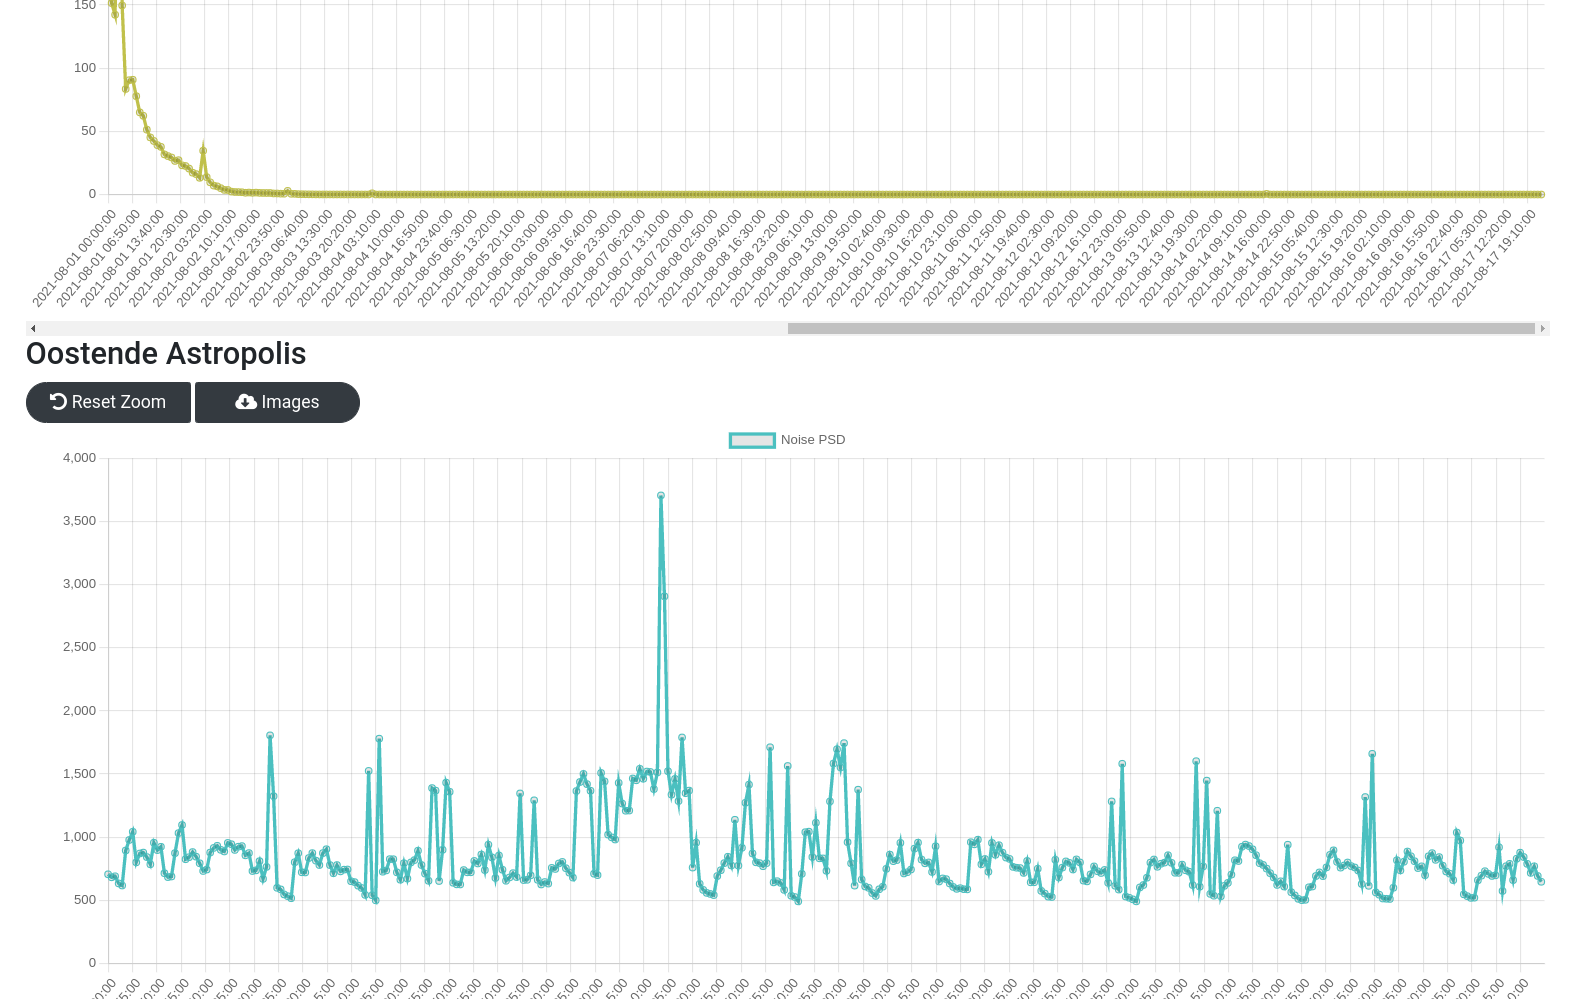
\includegraphics[scale=0.21]{Screenshot from 2022-08-22 10-49-20.png}
    \end{center}
\end{figure}

\begin{figure}[H]
    \begin{center}
        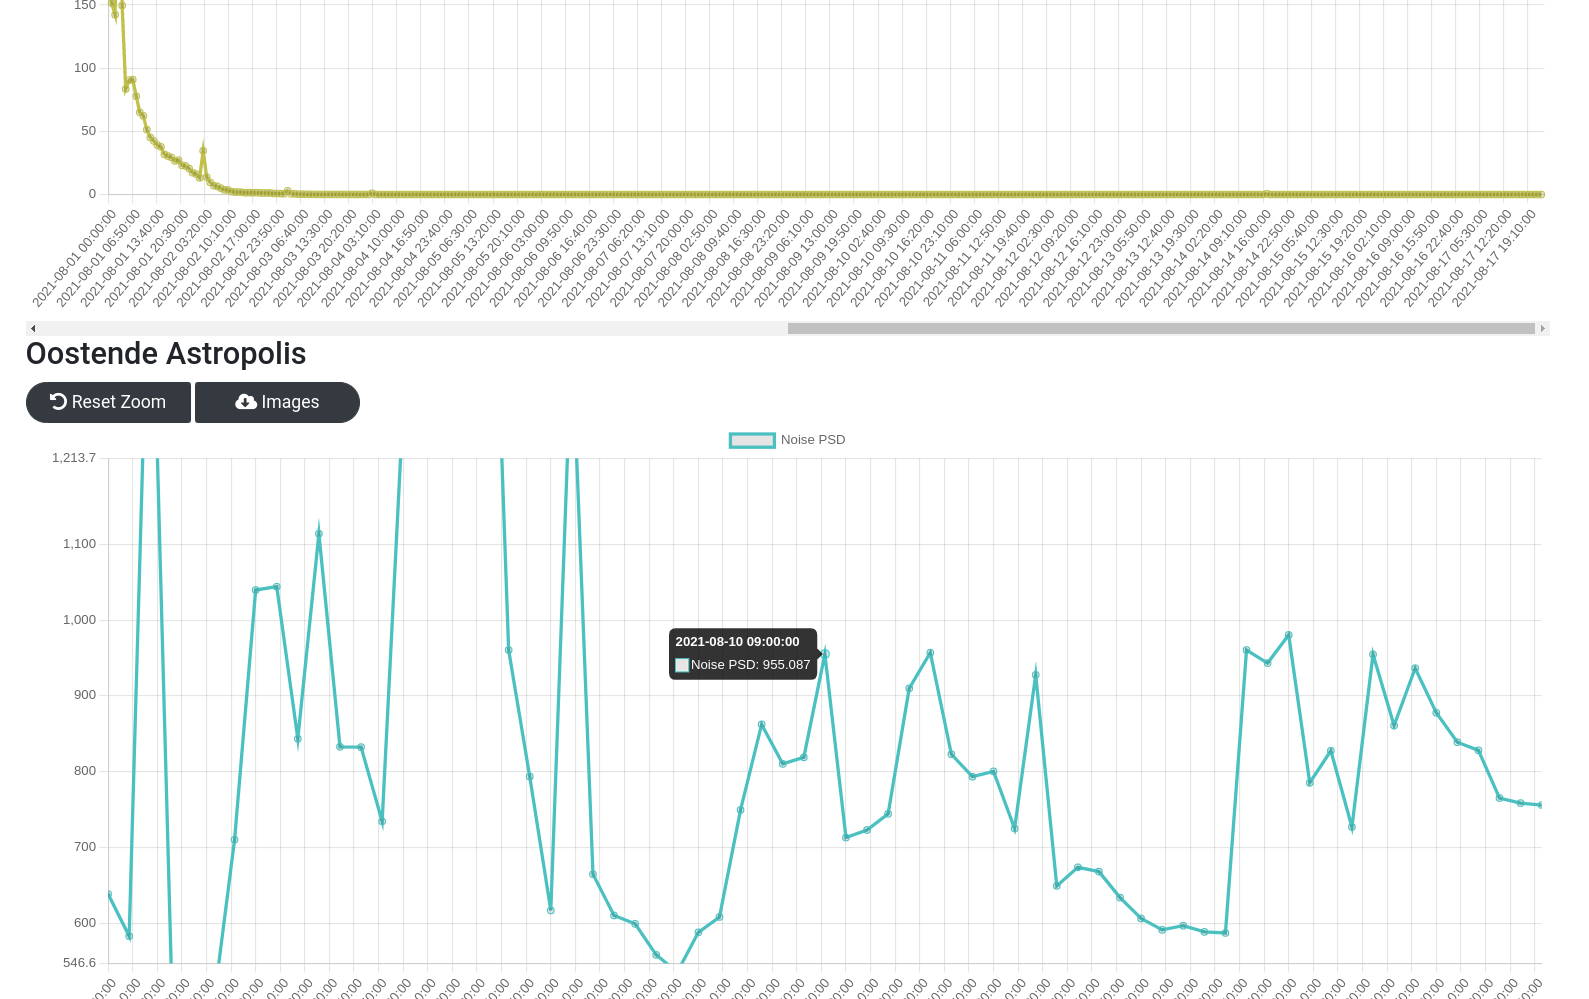
\includegraphics[scale=0.21]{Screenshot from 2022-08-22 10-49-34.png}
    \end{center}
\end{figure}

\newpage

\section{Kernel de Convolution Permettant d'Amplifier les Signaux de Météores} \label{app:kernel}

\begin{lstlisting}[style=CStyle]
       [[ 0.   0.   0.  50.   0.   0.   0. ]
        [ 0.   0.   0.  50.   0.   0.   0. ]
        [ 0.   0.   0.   0.   0.   0.   0. ]
        [ 0.   0.   0.   0.   0.   0.   0. ]
        [ 0.   0.   0.   0.   0.   0.   0. ]
        [ 0.   0.   0.   0.   0.   0.   0. ]
        [ 0.   0.   0.   0.   0.   0.   0. ]
        [ 0.   0.   0.   0.   0.   0.   0. ]
        [ 0.   0.   0.   0.   0.   0.   0. ]
        [ 0.   0.   0.   0.   0.   0.   0. ]
        [ 0.   0.   0.   0.   0.   0.   0. ]
        [ 0.   0.   0.   0.   0.   0.   0. ]
        [-1.5  0.   0.   0.   0.   0.  -1.5]
        [-1.5  0.   0.   0.   0.   0.  -1.5]
        [-1.5  0.   0.   0.   0.   0.  -1.5]
        [ 0.   0.   0.   0.   0.   0.   0. ]
        [ 0.   0.   0.   0.   0.   0.   0. ]
        [ 0.   0.   0.   0.   0.   0.   0. ]
        [ 0.   0.   0.   0.   0.   0.   0. ]
        [ 0.   0.   0.   0.   0.   0.   0. ]
        [ 0.   0.   0.   0.   0.   0.   0. ]
        [ 0.   0.   0.   0.   0.   0.   0. ]
        [ 0.   0.   0.   0.   0.   0.   0. ]
        [ 0.   0.   0.   0.   0.   0.   0. ]
        [ 0.   0.   0.   0.   0.   0.   0. ]
        [ 0.   0.   0.  50.   0.   0.   0. ]
        [ 0.   0.   0.  50.   0.   0.   0. ]]
\end{lstlisting}

\newpage

\section{Résultat du filtre pour amplifier les échos de météores} \label{app:spectro-mod1}

\begin{figure}[h]
    \begin{center}
        \includegraphics[scale=0.13]{spectro_mod1.png}
    \end{center}
\end{figure}

\section{Résultat du filtre à percentile} \label{app:spectro-mod2}

\begin{figure}[H]
    \begin{center}
        \includegraphics[scale=0.13]{spectro_mod2.png}
    \end{center}
\end{figure}

\newpage

\section{Résultat des éléments étant trop petits pour pouvoir être un écho} \label{app:spectro-mod3}

\begin{figure}[h]
    \begin{center}
        \includegraphics[scale=0.13]{spectro_mod3.png}
    \end{center}
\end{figure}

% \section{Méthode FFT de la Classe BramsWavFile}

% \begin{lstlisting}[style=CStyle]
% def FFT(self, Isamples, force_new=False):
%     if (
%         self.fft is not None
%         and self.fft_fbin is not None
%         and self.fft_freq is not None
%         and not force_new
%     ):
%         return self.fft_freq, self.fft, self.fft_fbin

%     # get the length of all the audio samples
%     nsamples = Isamples.size

%     # create a window funtion
%     w = windows.hann(nsamples)
%     w_scale = 1 / w.mean()

%     # apply that window on all the audio samples
%     Isamples = Isamples * w * w_scale

%     # get the Fourier Tranform and normalize it
%     S = rfft(Isamples) / nsamples
%     S[1: -1] *= 2

%     self.fft = S
%     self.fft_fbin = self.fs / nsamples
%     self.fft_freq = rfftfreq(nsamples, 1 / self.fs)

%     return self.fft_freq, S, self.fft_fbin
% \end{lstlisting}


\end{document}